%!TEX root = ../DSGEnotes.tex
\begin{subappendices}

  \section{超几何方程}
  \label{sec:hypergeometricfunctions}
  \begin{definition}[超几何序列]
    一组序列$\{c_n\}$,如果$\frac{c_{n+1}}{c_{n}}$是一个关于$n$的有理方程,则我们称$\{c_n\}$是一个超几何序列(Hypergeometric Series)\index{hypergeometric!series \dotfill 超几何序列}。
  \end{definition}

以阶乘形式表示为
\begin{equation}
\label{eq:hgf-hgf-series-fact}
\frac{c_{n+1}}{c_{n}} = \frac{\left(n+a_1\right) \left(n+a_2\right) \ldots \left(n+a_p\right)}{\left(n+b_1\right) \left(n+b_2\right) \ldots \left(n+b_q\right)} \frac{z}{\left(n+1\right)}, \quad n=0,1,2\ldots,
\end{equation}
如果$z=1$,$\{c_n\}$又称首一超几何序列(monic hypergeometric series)\index{hypergeometric!series, monic \dotfill 首一超几何序列};如果$z \neq 1$,则称非首一超几何序列。分母中的$n+1$项可以是来自阶乘本身,也可以不是,对于后者的情况,我们也可以在分子中加入一个额外的$(n+a_i)$项予以调节,即选取一个$i \in 0,1 \ldots n+1$使得$a_i = 1$。

对\eqref{eq:hgf-hgf-series-fact}做迭代我们有
\begin{equation}
\label{eq:hgf-hgf-series-iteration}
c_n = \frac{\left(a_1\right)_n \left(a_2\right)_n \ldots \left(a_p\right)_n}{\left(b_1\right)_n \left(b_1\right)_n \ldots \left(b_q\right)_n} \frac{z^n}{n!} c_0,
\end{equation}
其中$n!$表示$n$的阶乘。 $\left(a_1 \right)_n$表示伯赫哈默尔符号(Pochhammer symbol)\index{Pochhammer symbol \dotfill 伯赫哈默尔符号}的定义如下
\begin{equation*}
  \left(a_1 \right)_n := \begin{cases}
  1 & \quad \text{如果 } n=0,\\
   a_1 (a_1 + 1) (a_1 + 2) \ldots (a_1 + n -1) & \quad \text{如果 }n=1,2,3 \ldots.
  \end{cases}
\end{equation*}

对超几何序列$\{c_n\}$的求和为
\begin{equation*}
  \sum_{n=0}^{\infty} c_n = c_0 \sum_{n=0}^{\infty}  \frac{\left(a_1\right)_n \left(a_2\right)_n \ldots \left(a_p\right)_n}{\left(b_1\right)_n \left(b_1\right)_n \ldots \left(b_q\right)_n} \frac{z^n}{n!},
\end{equation*}
这引出超几何方程的定义。

\begin{definition}[超几何方程]
  超几何方程(hypergeometric function)\index{hypergeometric!function \dotfill 超几何方程}$\Hypergeometric{p}{q}{a}{b}{x}$定义为超几何序列$\{c_n\}$的和:
  \begin{equation}
    \label{eq:hgf-hgf-function}
    \Hypergeometric{p}{q}{a}{b}{x} = \sum_{k=0}^{n} c_n = \sum_{n=0}^{\infty} \frac{\left(a_1\right)_n \left(a_2\right)_n \ldots \left(a_p\right)_n}{\left(b_1\right)_n \left(b_1\right)_n \ldots \left(b_q\right)_n} \frac{z^n}{n!}
  \end{equation}
\end{definition}
显然,上式成立要求分母的系数$\neq 0$。对于分子的系数,如果某一个$i$次系数$a_i=-N$,其中$N$是个非负整数,那么超几何方程$\Hypergeometric{p}{q}{a}{b}{x}$是一个关于$z$的多项式, 详见定义\ref{definition:hgf-generalized-definition};反之,则超几何序列的收敛速度$\rho$满足
\begin{equation*}
  \rho = \begin{cases}
  \infty &\quad \text{ 如果 } \,p < q+1, \\
  1 &\quad \text{ 如果 }\,p = q+1,\\
  0 &\quad \text{ 如果 }\,p > q+1,
  \end{cases}
\end{equation*}
这是由超几何序列的性质所决定的:由\eqref{eq:hgf-hgf-series-fact}可得
\begin{equation*}
  \lim_{n \rightarrow \infty} \left| \frac{c_{n+1}}{c_{n}} \right|= \begin{cases}
  \infty & \quad \text{ 如果 }\, p < q+1, \\
  \left| z \right| &\quad \text{ 如果 }\,p = q+1,\\
  \infty &\quad \text{ 如果 }\,p > q+1,
  \end{cases}
\end{equation*}
我们最为关注$p=q+1$的情况:随着$\left| z \right|$的取值不同,超几何函数$\Hypergeometric{q+1}{q}{a}{b}{z}$呈现出不同的收敛特点:
\begin{equation*}
  \Hypergeometric{q+1}{q}{a}{b}{z} \begin{cases}
  \text{收敛,} & \quad \text{如果}\, \left| z \right| < 1,\\
  \text{收敛,} & \quad \text{如果}\, \left| z \right| = 1, Re \left( \sum^{q} b_i - \sum^{q+1} a_j \right) >0,\\
  \text{有条件收敛,} & \quad \text{如果}\, \left| z \right| = 1, z \neq -1, -1 < Re \left( \sum^{q} b_i - \sum^{q+1} a_j \right) \le 0, \\
  \text{不收敛,} & \quad \text{如果}\, Re \left( \sum^{q} b_i - \sum^{q+1} a_j \right) \le -1.
  \end{cases}
\end{equation*}

\begin{definition}[广义超几何方程]
  \label{definition:hgf-generalized-definition}
  广义超几何方程(generalized hypergeometric function)\index{hypergeometric!function, generalized \dotfill 广义超几何方程}是超几何方程的一种特殊形式,定义式为
  \begin{equation}
    \label{eq:hgf-generalized-definition}
    \Hypergeometric{2}{1}{a,b}{c}{z} = \sum_{n=0}^{\infty} \frac{\left( a \right)_n \left( b \right)_n}{\left( c \right)_n} \frac{z^n}{n!},
  \end{equation}
\end{definition}
其中如果$a=-N, \, N=0,1,2\ldots$,那么我们有
\begin{equation*}
  \left( a \right)_n = \left( -N \right)_n = \left( -N \right)\left( -N +1 \right) \left( -N +2 \right) \ldots \left( -N + n -1 \right) = 0, \, n=N+1, N+2, N+3 \ldots.
\end{equation*}
那么\eqref{eq:hgf-generalized-definition}变为
\begin{equation}
  \label{eq:hgf-generalized-definition-N}
  \Hypergeometric{2}{1}{-N,b}{c}{z} = \sum_{n=0}^{N} \frac{\left(-N \right)_n \left( b \right)_n}{\left( b \right)_n} \frac{z^n}{n!}, \quad N=0,1,2 \ldots.
\end{equation}

如果${a_n}$不是个常数,那么超几何序列想要获得收敛特性,需要满足如下情况,第一种情况是$\left| z \right| <1$,第二种情况是$\left| z \right| = 1$以及$Re(c-a-b) >0$。

许多函数都可以表示为超几何方程的形式。如
\begin{equation*}
  \ln(1+x) = \sum_{n=0}^{\infty} \frac{(-1)^n}{n+1} x^{n+1} = \sum_{n=0}^{\infty} \frac{(1)_n (1)_n}{(2)_n} \frac{(-1)^n x^{n+1}}{n!}= \sum_{n=0}^{\infty} \frac{n! \, n!}{(n+1)!} \frac{(-1)^n x^{n+1}}{n!} = x \, \pFq{2}{1}{1,1}{2}{-x},
\end{equation*}

\begin{equation*}
\begin{split}
  \arctan{x} &= \sum_{n=0}^{\infty} \frac{(-1)^n}{2n+1} x^{2n+1} = \sum_{n=0}^{\infty} \frac{\left(\frac{1}{2}\right)_n (1)_n}{\left(\frac{3}{2}\right)_n} \frac{(-1)^n x^{2n+1}}{n!} = x \, \pFq{2}{1}{\frac{1}{2},1}{\frac{3}{2}}{-x^2}, \\
  &\text{最后一个等式是由于}\frac{\left(\frac{1}{2}\right)_n}{\left(\frac{3}{2}\right)_n} = \frac{\frac{1}{2}\frac{3}{2} \ldots \frac{2n-1}{2}}{\frac{3}{2}\frac{5}{2} \ldots \frac{2n+1}{2}} = \frac{\frac{1}{2}}{\frac{2n+1}{2}} = \frac{1}{2n+1}
\end{split}
\end{equation*}

\begin{theorem}[二项式定理]
  作为超几何方程的特殊形式之一,可以写成如下形式,称为二项式定理(binomial theorem)\index{binomial theorem \dotfill 二项式定理}
  \begin{equation}
    \label{eq:hgf-binomial-theorem}
    \pFq{2}{1}{a,b}{b}{z}=\pFq{1}{0}{a}{\_}{z} = \sum_{n=0}^{\infty} \frac{(a)_n}{n!}z^n = \sum_{n=0}^{\infty} \begin{pmatrix} -a \\ n \end{pmatrix}\frac{(a)_n}{n!}(-z)^n = (1-z)^{-a}, \quad \left| z \right|<1.
  \end{equation}
\end{theorem}

以及还有一类特殊的超几何方程
\begin{equation}
  \pFq{0}{0}{\_}{\_}{z}=\sum_{t=0}^{\infty} \frac{z^n}{n!} = e^z, \quad z \in \mathbb{C}.
\end{equation}

以及当系数趋近于无穷时:
\begin{align*}
%  \begin{split}
    &\lim_{b \rightarrow \infty} \pFq{2}{1}{a,b}{c}{\frac{z}{b}} = \lim_{b \rightarrow \infty} \sum_{n=0}^{\infty} \frac{(a)_n z^n}{(c)_n n!} \frac{(b)_n}{b^n} = \sum_{n=0}^{\infty} \frac{(a)_n}{(c)_n} \frac{z^n}{n!} = \pFq{1}{1}{a}{c}{z}, \\
    &\lim_{c \rightarrow \infty} \pFq{2}{1}{a,b}{c}{cz} =
    \lim_{c \rightarrow \infty} \sum_{n=0}^{\infty} \frac{(a)_n (b)_n}{n!} z^n \frac{c^n}{(c)_n} = \sum_{n=0}^{\infty} (a)_n \, (b)_n \, \frac{z^n}{n!} = \pFq{2}{0}{a,b}{\_}{z}.
%    \end{split}
\end{align*}

\begin{theorem}[超几何方程与欧拉积分表达式的转换]
  如果$Re (c) > Re (b) > 0$,那么对于沿着从$1$到$\infty$实数轴展开的所有 $z \in \mathbb{C}$,满足$\arg t = \arg (1-t) = 0$并且$(1-z t)^{-a}$有主值(principal value)的条件\footnote{膏按:反正这一串前提限定条件我没看懂...我的理解是,经济学研究中,能够熟悉下面的转换公式就可以了——这真是一本不负责任的``讲义''啊...},我们可以将超几何方程转换为欧拉积分表达式(Euler's integral representation)\index{Euler integral representation \dotfill 欧拉积分表达式}
  \begin{equation}
    \label{eq:hgf-euler-integral-transformation}
    \pFq{2}{1}{a,b}{c}{z} = \frac{\Gamma(c)}{\Gamma(b) \Gamma(c-b)} \int_{0}^{1} t^{b-1} (1-t)^{c-b-1} (1-z t)^{-a} \, dt.
    \end{equation}
\end{theorem}
\begin{proof}
  假设$\left| z \right| <1$,那么由二项式定理\eqref{eq:hgf-binomial-theorem}可得
  \begin{equation*}
    (1-z t)^{- a} = \sum_{n=0}^{\infty} \frac{(a)_n}{n!} z^n t^n,
  \end{equation*}
  这表明
  \begin{equation*}
    \int_{0}^{t} t^{b-1} (1-t)^{c-b-1} (1-z t)^{-a} dt = \underbrace{\sum_{n=0}^{\infty} \frac{(a)_n}{n!} z^n t^n}_{\text{RHS甲}} \underbrace{\int_{0}^{t} t^{b-1} (1-t)^{c-b-1} dt}_{\text{RHS乙}},
  \end{equation*}
  RHS分为两部分。乙是一个贝塔积分(Beta integral)\index{Beta integral \dotfill 贝塔积分},满足条件\footnote{
  其中$\Gamma(\cdot)$是Gamma方程\index{Gamma function \dotfill{伽马方程}},是阶乘函数在实数与复数上的扩展,定义为
  \begin{equation*}
    \Gamma(a) =\begin{cases}
    (n-1)! & \text{n是正整数}, \\
    \int_0^{\infty} t^{a-1} \exp(-t)  \, dt & z \in \mathbb{C}, Re(c) >0.
    \end{cases}
  \end{equation*}
  }
  \begin{equation*}
    \int_{0}^{t} t^{b-1} (1-t)^{c-b-1} dt = B(n+b, c-b) = \frac{\Gamma(n+b) \Gamma(c-b)}{\Gamma(n+c)}.
  \end{equation*}
此外Gamm方程可以转换为Pochhammer符号\index{Pochhammer symbol \dotfill 伯赫哈默尔符号}的表达形式:
\begin{equation*}
  \frac{\Gamma(n+b)}{\Gamma(b)} = b (b+1) (b+2) \ldots (b + n - 1) = (b)_n,
\end{equation*}
那么
\begin{equation*}
  \frac{\Gamma(n+b) \Gamma(c-b)}{\Gamma(n+c)} = \Gamma(c-b) \frac{\Gamma(b)}{\Gamma(c)} \frac{(b)_n}{(c)_n},
\end{equation*}
作为RHS乙代回原式有
\begin{equation*}
\frac{\Gamma(c)}{\Gamma(b) \Gamma(c-b)} \int_{0}^{t} t^{b-1} (1-t)^{c-b-1} (1-z t)^{-a} \, dt = \sum_{0}^{\infty} \frac{(a)_n \, (b)_n}{(c)_n} \frac{z^n}{n!} = \pFq{2}{1}{a,b}{c}{z}.
\end{equation*}
\end{proof}

\begin{theorem}[欧拉积分表达式与高斯求和公式的转换]对于$Re(c-a-b)>0$,我们有欧拉积分表达式与高斯求和公式(Gauss summation formula)\index{Gauss summation formula \dotfill{高斯求和公式}}的转换
  \begin{equation}
    \label{eq:hgf-euler-gauss}
    \pFq{2}{1}{a,b}{c}{1}=\frac{\Gamma(c) \, \Gamma(c-a-b)}{\Gamma(c-a) \, \Gamma(c-b)}.
  \end{equation}
\end{theorem}
\begin{proof}
  假设$\lim_{z \rightarrow 1}$,通过\eqref{eq:hgf-euler-integral-transformation}我们有
  \begin{equation*}
    \begin{split}
      &\lim_{z \rightarrow 1}\pFq{2}{1}{a,b}{c}{z} \approx \pFq{2}{1}{a,b}{c}{1} = \frac{\Gamma(c)}{\Gamma(b) \, \Gamma(c-b)} \, \int_{0}^{1} t^{b-1} (1-t)^{c-a-b-1} \, dt \\
      &=\frac{\Gamma(c)}{\Gamma(b) \, \Gamma(c-b)} \, B(b,c-a-b) = \frac{\Gamma(c)}{\Gamma(b) \, \Gamma(c-b)} \, \frac{\Gamma(b) \Gamma(c-a-b)}{\Gamma(c-a)} = \frac{\Gamma(c) \Gamma(c-a-b)}{\Gamma(c-a) \Gamma(c-b)}.
    \end{split}
  \end{equation*}
\end{proof}

\begin{theorem}[高斯求和公式与朱世杰——范德蒙德求和公式的转换]
  当$a=-n, n \in \{0,1,2\ldots\}$(并且$\lim_{z \rightarrow 1}$)时,高斯求和公式\eqref{eq:hgf-euler-gauss}缩减成为朱世杰——范德蒙德求和公式(Chu-Vandermonde summation)\index{Chu-Vandermonde summation \dotfill 朱世杰——范德蒙德求和公式}
  \begin{equation}
    \pFq{2}{1}{-n,b}{c}{1}=\frac{(c-b)_n}{(c)_n}, n=0,1,2\ldots.
  \end{equation}
\end{theorem}
\begin{proof}
  \begin{equation*}
    \frac{\Gamma(c) \Gamma(c-a-b)}{\Gamma(c-a) \Gamma(c-b)} = \frac{\Gamma(c) \Gamma(c-b+n)}{\Gamma(c+n) \Gamma(c-b)} = \frac{(c-b)_n}{c(n)}.
  \end{equation*}
\end{proof}

\begin{theorem}[超几何方程与法夫转换公式]
  我们可以用欧拉积分表达式证明,超几何方程可以写成法夫转换公式(Pfaff's transformation formula)\index{Pfaff's transformation formula \dotfill 法夫转换公式}的形式
  \begin{equation}
    \label{eq:hpf-pfaff-trans}
    \pFq{2}{1}{a,b}{c}{z}=(1-z)^{-a} \pFq{2}{1}{a,c-b}{c}{\frac{z}{z-1}}.
  \end{equation}
\end{theorem}
\begin{proof}
  定义$t=1-s$,代入欧拉积分表达式\eqref{eq:hgf-euler-integral-transformation}我们有
  \begin{equation*}
    \begin{split}
      \pFq{2}{1}{a,b}{c}{z} &= \int_0^1 t^{b-1} (1-t)^{c-b-1} (1-z t)^{-a} \, dt \\
      &= - \int_0^1 (1-s)^{b-1} s^{c-b-1} (1-z + z s)^{-a} \, ds \\
      &= (1-z)^{-a} \int_0^1 s^{c-b-1} (1-s)^{b-1} \left( 1 - \frac{z s}{z - 1} \right)^{-a} \, ds \\
      &= (1-z)^{-a} \pFq{2}{1}{a,c-b}{c}{\frac{z}{z-1}}.
    \end{split}
  \end{equation*}
\end{proof}

\begin{theorem}[超几何方程与欧拉转换公式]
  我们可以用法夫转换公式证明,超几何方程可以写成欧拉转换公式(Euler's transformation formula)\index{Euler transformation formula \dotfill 欧拉转换公式}的形式
  \begin{equation}
    \label{eq:hgf-euler-transformation-formula}
    \pFq{2}{1}{a,b}{c}{z} = (1-z)^{c-a-b} \pFq{2}{1}{c-a,c-b}{c}{z}.
  \end{equation}
\end{theorem}
\begin{proof}
  两次使用法夫转换公式
  \begin{equation*}
    \begin{split}
      \pFq{2}{1}{a,b}{c}{z} &= (1-z)^{a} \pFq{2}{1}{a,c-b}{c}{\frac{z}{z-1}} \\
      &= (1-z)^{a} (1-z)^{b-c} \pFq{2}{1}{c-a,c-b}{c}{\frac{\frac{z}{z-1}}{\frac{z}{z-1} - 1}}\\
      &=(1-z)^{c-a-b} \pFq{2}{1}{c-a,c-b}{c}{z}
    \end{split}
  \end{equation*}
\end{proof}

\begin{theorem}[法夫——萨尔舒茨求和公式]
  一个${}_{3}F_{2}$超几何方程又可以写成法夫——萨尔舒茨求和公式(Pfaff-Saalschütz summation formula)\index{Pfaff-Saalschütz summation formula \dotfill 法夫——萨尔舒茨求和公式}的形式
  \begin{equation}
    \label{eq:hgf-Pfaff-Saalschuetz}
    \pFq{3}{2}{-n,a,b}{c,1+a+b-c-n}{1} = \frac{(c-a)_n (c-b)_n}{(c)_n (c-a-b)_n}, \quad n=0,1,2\ldots.
  \end{equation}
\end{theorem}
\begin{proof}
  欧拉转换公式\eqref{eq:hgf-euler-transformation-formula}又可以写成
  \begin{equation*}
    (1-z)^{a+b-c} \pFq{2}{1}{a,b}{c}{z} = \pFq{2}{1}{c-a,c-b}{c}{z},
  \end{equation*}
  其中LHS$\rightarrow$
  \begin{equation*}
    \begin{split}
      (1-z)^{a+b-c} \pFq{2}{1}{a,b}{c}{z} &= \sum_{j=0}^{\infty} \frac{(c-a-b)_j}{j!} z^j \sum_{k=0}^{\infty} \frac{(a)_k (b)_k}{(c)_k} \frac{z^k}{k!} \\
      &=\sum_{n=0}^{\infty} \sum_{k=0}^{n} \frac{(a)_k (b)_k (c-a-b)_{n-k}}{(c)_k k! (n-k)!} z^n.
    \end{split}
  \end{equation*}
  RHS$\rightarrow$
  \begin{equation*}
    \pFq{2}{1}{c-a,c-b}{c}{z} = \sum_{n=0}^{\infty}
    \frac{(c-a)_n (c-b)_n}{(c)_n} \frac{z^n}{n!}.
  \end{equation*}

  比较两个式子中$z^n$对应的系数,我们有
  \begin{equation*}
    \sum_{k=0}^{n} \frac{(a)_k (b)_k (c-a-b)_{n-k}}{(c)_k k! (n-k)!} z^n = \frac{(c-a)_n (c-b)_n}{(c)_n n!}, \quad n=0,1,2 \ldots, \quad k\in \{0,1,2, \ldots n\}.
  \end{equation*}
\end{proof}

其中由于
\begin{align*}
  \frac{n!}{(n-k)!} = n(n-1)\ldots(n-k+1) = (-1)^k (-n) (-n+1) \ldots (-n + k -1) = (-1)^k (-n)^k,
\end{align*}
以及
\begin{align*}
  (c-a-b)_{n-k} &= \frac{
  (c-a-b)_n
  }{
  (c-a-b+n-k)(c-a-b+n-k-1)\ldots(c-a-b+n-1)
  } \\
  &=\frac{(c-a-b)_n}{(-1)^k (1+a+b-c-n)_k}.
\end{align*}

因此
\begin{equation*}
  \sum_{k=0}^{n} \frac{(a)_k (b)_k (-n)_{k}}{(c)_k k! (1+a+b-c-n)_k} = \frac{(c-a)_n (c-b)_n}{(c)_n (c-a-b)_n}, \quad n=0,1,2 \ldots, \quad k\in \{0,1,2, \ldots n\},
\end{equation*}
进而\eqref{eq:hgf-Pfaff-Saalschuetz}成立。

\begin{theorem}[法夫——萨尔舒茨求和公式与高斯求和公式的转换]
随着$n \rightarrow \infty$,${}_3{F}_{2}$的法夫——萨尔舒茨求和公式\eqref{eq:hgf-Pfaff-Saalschuetz}逐渐缩减到${}_2{F}_{1}$的高斯求和公式\eqref{eq:hgf-euler-gauss}的形式
\begin{equation}
  \label{eq:pfaff-schuetz-gauss-transform}
  \lim_{n\rightarrow \infty} \pFq{3}{2}{-n,a,b}{c,1+a+b-c-n}{1}=\pFq{2}{1}{a,b}{c}{1}.
\end{equation}
\end{theorem}
\begin{proof}
  根据
  \begin{equation*}
    (a)_n = a (a+1) \ldots (a+n-1) = \frac{\Gamma(a+n)}{\Gamma(a)},
  \end{equation*}
  我们有
  \begin{equation*}
    \begin{split}
          \frac{(c-a)_n (c-b)_n}{(c)_n (c-a-b)_n} &= \frac{
          \Gamma(c-a+n) \Gamma(c-b+n) \Gamma(c) \Gamma(c-a-b)
          }{
          \Gamma(c-a) \Gamma(c-b) \Gamma(c+n) \Gamma(c-a-b+n)
          } \\
          &= \frac{\Gamma(c) \Gamma(c-a-b)}{\Gamma(c-a) \Gamma(c-b)}
          \underbrace{\frac{\Gamma(c-a+n) \Gamma(c-b+n)}{\Gamma(c+n) \Gamma(c-a-b+n)}},
    \end{split}
  \end{equation*}
  上式中下括号部分可由斯特灵公式(Stirling formula)近似:
  \begin{equation*}
    \lim_{n \rightarrow 0} \frac{\Gamma(c-a+n) \Gamma(c-b+n)}{\Gamma(c+n) \Gamma(c-a-b+n)} \sim n^{c-a+c-b-c-c+a+b} = n^0 = 1,
  \end{equation*}
  即
  \begin{equation*}
    \lim_{n \rightarrow \infty} \frac{(c-a)_n (c-b)_n}{(c)_n (c-a-b)_n} = \frac{\Gamma(c) \Gamma(c-a-b)}{\Gamma(c-a) \Gamma(c-b)},
  \end{equation*}
  由此得到
  \begin{equation*}
    \begin{split}
          \pFq{2}{1}{a,b}{c}{1}&=\lim_{n\rightarrow \infty}\pFq{3}{2}{-n,a,b}{c,1+a+b-c-n}{1}\\
          &=\lim_{n \rightarrow \infty} \frac{(c-a)_n (c-b)_n}{(c)_n (c-a-b)_n} \\
          &=\frac{\Gamma(c) \Gamma(c-a-b)}{\Gamma(c-a) \Gamma(c-b)}.
    \end{split}
  \end{equation*}
\end{proof}

\section{多项式}
\label{sec:poly}

\subsection{正交集}
数学意义上来说,正交(orthogonal)意味着垂直(perpendicular)。如,一个三维向量空间中的向量集$\{x,y,z\}$是正交的,意思就是说任意两个正交向量的点乘(dot product)都为零,$x.y=0,x.z=0,y.z=0$。因此我们又将$\{x,y,z\}$称为正交集合。在$\{x,y,z\}$构成的三维空间中,任何一点都可以表示为$x,y$或$z$向量中的一项——换句话说,$\{x,y,z\}$共同构成了一个三维空间的基(basis)。

如果$\{x,y,z\}$都是单位向量,则进一步称之为标准正交向量集。

\begin{definition}[黎曼——斯蒂尔杰斯积分]
  在区间$[a,b]$内,假定对于一个实变量$\lambda$的实函数$\alpha(\lambda)$,存在一个对应的实函数$f(\lambda)$,则黎曼——斯蒂尔杰斯积分(Riemann-Stieltjes integral)\index{Riemann-Stieltjes integral \dotfill 黎曼——斯蒂尔杰斯积分}$\int_{a}^{b} f(\lambda) \, d \alpha(\lambda)$描述了当将区间$[a,b]$分割为无限多个块(数量用$\pi$表示)时,下述和的极限值
\begin{equation}
  \label{eq:poly-riemann-sitltjes-def}
  \int_a^b f(\lambda) \, d \alpha(\lambda) = \sum_{\lambda_i \in \pi } f(c_i) \left( \alpha(\lambda_{i+1}) - \alpha(\lambda_{i})\right), \quad c_i \in [\lambda_{i+1}, \lambda_{i}].
\end{equation}
\end{definition}
黎曼——斯蒂尔杰斯积分值若要存在,需要$f(\cdot)$是连续方程,以及非递减方程$\alpha(\cdot)$在$[a,b]$中有界。

黎曼——斯蒂尔杰斯积分常常直接写作简化形式
\begin{equation}
  \label{eq:poly-riemann-sitltjes-def-simp}
  \int_a^b f(\lambda) w(\lambda) \, d \lambda,
\end{equation}
其中$w(\cdot)$称权重方程(weight function\index{weight function \dotfill 权重方程})。

\subsection{正交多项式}
任意一个无限多项式序列$\{p_{n}(\lambda)\}_{n=0}^{\infty}$向量(其中$p_{n}(\lambda)$表示其中的第n次多项式),都构成无限维度向量空间中的一个基。
\begin{definition}[正交多项式]
  如果一个多项式序列$\{p_n(\lambda)\}_{n=0}^{\infty}$ 在区间$(a,b)$中,关于权重方程$w(\lambda)$,满足如下关系,那么我们说它是正交多项式(orthogonal polynomial):
  \begin{equation}
    \label{eq:poly-orthogonal-poly-def}
    \int_a^b w(\lambda) p_m(\lambda) p_n(\lambda) d \lambda = h_n \delta_{mn}
  \end{equation}
\end{definition}
  \begin{itemize}
    \item $h_n$ 称范数(norm)\index{norm \dotfill 范数}  ,正交多项式$p(\lambda)$的范数也表示为$\left| p \right|$,定义为(具体细节见第\ref{sec:lp-norm}。)
    \begin{equation}
      \label{eq:poly-norm-def}
      h_n = \left| p_{n}(\lambda) \right| = \int_a^b w(\lambda) p_n(\lambda)^2 \, d x >0, n=0,1,2\ldots
    \end{equation}
    \item 权重方程$w(\lambda)$应当在$(a,b)$区间内连续且为正,以使矩(moment) $\mu_n$存在。
    \item 矩(moment)\index{moment \dotfill 矩} $\mu_n$定义为
    \begin{equation}
    \label{eq:poly-moment-def}
    \mu_n = \int_a^b w(x) \lambda^n \, d \lambda, \quad i=0,1,2\ldots
  \end{equation}
    \item $\delta_{mn}$是克罗内克(Kronecker product) \index{Kronecker product\dotfill 克罗内克乘积},表达如下关系
    \begin{equation}
      \label{eq:poly-kronecker}
      \delta_{m,n} = \begin{cases}
      0 & m \neq n, \\
      1 & m=n.
      \end{cases}
    \end{equation}
    \item 积分$\langle f, g \rangle$表示多项式$f$和$g$的内积(inner product)\index{inner product \dotfill 内积}
    \begin{equation}
      \label{eq:poly-inner-product-def}
      \langle p,q \rangle =
      \int_a^b w(\lambda) f(\lambda) g(\lambda) \, d \lambda.
    \end{equation}
    \item 区间$(a,b)$称正交区间(可以是一个无限区间,即$a \rightarrow -\infty, \, b \rightarrow +\infty$)。
  \end{itemize}

如果正交多项式$\{p_n(\lambda)\}_{n=0}^{\infty}$对于$k =0,1,2 \ldots n$都有$h_k = 1$,则称标准正交多项式(orthonormal polynomial)\index{polynomial!orthonormal \dotfill 标准正交多项式}。

如果第n次多项式$p_n(\lambda)=k_n \lambda^n + \chi$,其中$\chi$表示低于n次的其他项,并且对于每一个$n=0,1 \ldots $ 都有 $k_n = 1$,则称首一正交多项式(monic orthogonal polynomial)\index{polynomial!monic orthogonal \dotfill 首一正交多项式}。

标准正交多项式$p_n(\lambda)$和首一正交多项式$\hat{p}_n(\lambda)$之间可以相互转换(如见定理\ref{theorem:poly-orthonormal-recurrence-theorem})。
\begin{equation}
  \label{eq:poly-monic-orthonormal-transformation}
  \hat{p}_n(\lambda) = \frac{p_n(\lambda)}{\sqrt{\langle p_n(\lambda), p_n(\lambda)\rangle}}.
\end{equation}

我们可以根据格拉姆-施密特正交化过程(Gram-Schmidt orthogonality process)\index{Gram-Schmidt orthogonality process \dotfill 格拉姆-施密特正交化过程},把正交多项式序列$\{p_{n}(\lambda)\}_{n=0}^{\infty}$转化为正交集合。举例说明,取$w(\lambda)=1, \, (a,b)=(0,1), \, p_{0}(\lambda)=1$,求首一多项式序列$\{p_{n}(\lambda)\}$。

从序列$\{1,\lambda, \lambda^2 \ldots \}$开始。第一步求$p_1(\lambda)$
\begin{equation*}
  \begin{split}
    p_1(\lambda) &= \lambda - \frac{\langle \lambda, p_{0}(\lambda) \rangle}{\langle p_{0}(\lambda) \lambda, p_{0}(\lambda) \rangle} \, p_0(\lambda) \\
    &= \lambda - \frac{\langle \lambda,1 \rangle }{\langle 1,1 \rangle} \\
    &= \lambda - \frac{
    \int_0^1 w(\lambda) \left(\lambda  \cdot 1 \right) \, d \lambda
    }{
    \int_0^1 w(\lambda) \left(1 \cdot 1 \right) \, d \lambda
    }\\
    &= \lambda - \frac{1}{2}.
  \end{split}
\end{equation*}

  第一步求$p_2(\lambda)$
  \begin{equation*}
    \begin{split}
      p_2(\lambda) &= \lambda^2 - \frac{\langle \lambda^2, p_0(\lambda) \rangle}{\langle p_0(\lambda),p_0(\lambda)\rangle} \, p_0(\lambda)
      - \frac{
      \langle \lambda^2, p_1(\lambda) \rangle
      }{
      \langle p_1(\lambda),p_1(\lambda)\rangle
      } \, p_1(\lambda) \\
      &= \lambda^2 - \frac{
      \langle \lambda^2, 1 \rangle
      }{
      \langle 1,1 \rangle
      } -\frac{
      \langle \lambda^2, \lambda-\frac{1}{2} \rangle
      }{
      \langle \lambda-\frac{1}{2}, \lambda-\frac{1}{2} \rangle
      } \left(\lambda-\frac{1}{2} \right)\\
      &=\lambda^2 - \frac{\frac{1}{3}}{1} - \frac{\frac{1}{12}}{\frac{1}{12}} \left( \lambda - \frac{1}{2} \right) \\
      &=\lambda^2 - \lambda + \frac{1}{6}.
    \end{split}
  \end{equation*}

则$p_0(\lambda)=1$,$p_1(\lambda)= \lambda - \frac{1}{2}$,$p_2(\lambda)=\lambda^2 - \lambda + \frac{1}{6}$就是首一正交多项式在(0,1)区间内,对应权重方程$w(\lambda)=1$的前三项。以此类推,可以继续求得$p_3(\lambda),p_4(\lambda) \ldots$
\begin{equation*}
  \begin{split}
    &p_3(\lambda) = \lambda^3 - \frac{3}{2} \lambda^2 + \frac{3}{5}\lambda - \frac{1}{20}, \\
    &p_4(\lambda) = \lambda^4 - 2 \lambda^3 + \frac{9}{7}\lambda^2 - \frac{2}{7} \lambda + \frac{1}{70}, \\
    &p_5(\lambda) = \lambda^5 - \frac{5}{2} \lambda^4 + \frac{20}{9} \lambda^3 - \frac{5}{6} \lambda^2 + \frac{5}{42} \lambda - \frac{1}{252} \ldots
  \end{split}
\end{equation*}

根据\eqref{eq:poly-norm-def}计算$h_n$;与首一正交多项式$p_n(\lambda)$对应的正交多项式$q_n(\lambda)$由\eqref{eq:poly-monic-orthonormal-transformation}给出
\begin{equation*}
  \begin{split}
    &q_1(\lambda) = \frac{p_1(\lambda)}{\sqrt{h_1}} = 2\sqrt{3} \left( x - \frac{1}{2} \right), \\
    &q_2(\lambda) = \frac{p_2(\lambda)}{\sqrt{h_2}} = 6 \sqrt{5} \left( x^2 - x + \frac{1}{6} \right), \\
    &q_3(\lambda) = \frac{p_3(\lambda)}{\sqrt{h_3}} = 20 \sqrt{7} \left( \lambda^3 - \frac{3}{2} \lambda^2 + \frac{3}{5}\lambda - \frac{1}{20} \right) \ldots
  \end{split}
\end{equation*}






















\subsubsection{正定}
如果$\left| p \right| >0, \, \left| q \right| >0, \, \forall p,q \in \mathbb{P}$,则$<.,.>$是正定的。换句话说,内积是正定的充分必要条件为,它的汉克尔矩阵(Hankel moment matrix)\index{Hankel moment matrix \dotfill 汉克尔矩阵}的行列式为正
\begin{equation}
  \label{eq:poly-hankel-moment-matrix-def}
  \det
  \begin{pmatrix}
    \mu_0 & \mu_1 & \mu_2 & \dots &\mu_{k-1} \\
    \mu_1 & \mu_2 & \mu_3 & \dots & \mu_k \\
    \vdots & \ddots & & & \vdots \\
    \mu_{k-1} & \mu_k & \mu_{k+1} & \dots & \mu_{2k-2}
  \end{pmatrix} >0, k=1,2,\ldots
\end{equation}
其中$\mu_i$的定义如\eqref{eq:poly-moment-def}所示。

\begin{theorem}[正交多项式的存在性]
  如果某内积$\langle.,.\rangle$在$\mathbb{P}$中正定,那么有且只有一个首一正交的无限多项式与每一个$\alpha(\lambda)$相对应。
\end{theorem}
\begin{proof}
  略。
\end{proof}

\begin{theorem}[正交多项式的最小化特性]
  如果$q_k(\lambda)$是一个$k$次的首一多项式,则只有当$q_k$等于一个常数与另一个同样关于$\alpha(\lambda)$的多项式$p_k$的乘积时,以下最小值才存在
  \begin{equation*}
    \min_{q_k} \int_a^b q_k(\lambda)^2 \, d \alpha(\lambda).
  \end{equation*}
\end{theorem}
\begin{proof}
  略。
\end{proof}

\subsection{递推关系}
\begin{theorem}[首一正交多项式的三项递推关系]
  \label{theorem:poly-recurrence-relation}
  对于首一正交多项式序列$\{ p_{n} (\lambda) \}$而言,存在着系数$\alpha_k$和$\gamma_k$,$k=1,2,\ldots$,使得其满足三项递推关系(three-term recurrence relation)\index{three-term recurrence relation!monic polynomial \dotfill 三项递推关系(首一正交多项式)}
  \begin{equation}
    \label{eq:poly-monic-poly-recurrence-def}
    \begin{split}
      &p_{k+1}(\lambda) = \left( \lambda - \alpha_{k+1} \right) p_{k}(\lambda) - \gamma_k p_{k-1}(\lambda) , \quad k = 1,2,\ldots, \\
      &p_{-1}(\lambda) :=0, \, p_{0}(\lambda) = 1, \\
      &\text{其中} \quad \alpha_{k+1} = \frac{\langle \lambda p_k, p_k \rangle}{\langle p_k,p_k \rangle}, \, \gamma_k = \frac{\langle p_k,p_k \rangle }{ \langle p_{k-1},p_{k-1} \rangle}.
    \end{split}
  \end{equation}
\end{theorem}

\begin{proof}
  对于$k =1,2,\ldots$设
  \begin{equation*}
    F(\lambda) := p_{k+1}(\lambda) - (\lambda - \alpha_{k+1}) p_{k}(\lambda) + \gamma_k \, p_{k-1}(\lambda),
  \end{equation*}
  由$p_{k-1},p_k,p_{k+1}$都是首一多项式可得$F(\lambda) \in \mathbb{P}_{n}[\lambda]$。此外,由$p_{k-1},p_k,p_{k+1}$的正交特性,我们分三种情况展开分析。

  第一种情况,当$0 < l < k-1$时,有
  \begin{equation*}
    \begin{split}
      \langle F(\lambda), p_{l}(\lambda) \rangle
      &= \underbrace{\langle p_{k+1}(\lambda),p_{l}(\lambda)\rangle}_{=0}
      - \underbrace{\langle p_{k}(\lambda), \left( \lambda - \alpha_{k+1} \right)p_{l}(\lambda) \rangle}_{=0}
      + \underbrace{\langle \gamma_k p_{k-1}(\lambda), p_{l}(\lambda)\rangle}_{=0} =0,
    \end{split}
  \end{equation*}
  其中用到了$\langle \lambda p, q \rangle = \langle p, \lambda q \rangle$,以及$\langle p_k,p_l \rangle =0, \, \forall \, 0 < l < k-1$。

  第二种情况,当$l = k-1$时,有
  \begin{equation*}
    \begin{split}
      \langle F(\lambda), p_{l}(\lambda) \rangle &= \langle F(\lambda), p_{k-1}(\lambda) \rangle \\
      &= \underbrace{\langle p_{k+1}(\lambda), p_{k-1}(\lambda) \rangle}_{=0} - \langle p_{k}(\lambda), \left( \lambda - \alpha_{k+1} \right) p_{k-1}(\lambda) \rangle
      + \langle \gamma_k p_{k-1}(\lambda), p_{k-1}(\lambda) \rangle \\
      &= -\langle p_{k}(\lambda), \lambda p_{k-1}(\lambda) \rangle
      + \underbrace{\langle p_{k}(\lambda), \alpha_{k+1} p_{k-1}(\lambda) \rangle}_{=0}
      +\gamma_k \langle p_{k-1}(\lambda), p_{k-1}(\lambda) \rangle = 0,
    \end{split}
  \end{equation*}
  因此我们有
  \begin{equation*}
    \gamma_k = \frac{
    \langle p_{k}(\lambda), p_{k}(\lambda) \rangle
    }{
    \langle p_{k-1}(\lambda), p_{k-1}(\lambda) \rangle
    }.
  \end{equation*}
  第三种情况,当$l=k$时,有
  \begin{equation*}
    \begin{split}
      \langle F(\lambda), p_{l}(\lambda) \rangle &= \langle F(\lambda), p_{k}(\lambda) \rangle \\
      &=\underbrace{\langle p_{k+1}(\lambda), p_{k}(\lambda) \rangle}_{=0}
      + \langle \left( -\lambda + \alpha_{k+1} \right) p_{k}(\lambda), p_{k}(\lambda) \rangle
      + \underbrace{\langle \gamma_k p_{k-1}(\lambda), p_{k}(\lambda) \rangle}_{=0} \\
      &=- \langle \lambda p_{k}(\lambda),p_{k}(\lambda) \rangle
      + \alpha_{k+1} \langle p_{k}(\lambda),p_{k}(\lambda) \rangle =0,
    \end{split}
  \end{equation*}
  因此我们有
  \begin{equation*}
    \alpha_{k+1} = \frac{
    \langle \lambda p_{k}(\lambda), p_{k}(\lambda)\rangle
    }{
    \langle p_{k}(\lambda), p_{k}(\lambda) \rangle
    }.
  \end{equation*}
\end{proof}

\begin{theorem}[标准正交多项式的三项递推关系]
  \label{theorem:poly-orthonormal-recurrence-theorem}
  对于标准正交多项式$\{p_{n} (\lambda)\}$而言,存在着系数$\alpha_k$和$\beta_{k}$,$k=0, 1,2,\ldots $,使得其满足三项递推关系(three-term recurrence relation)\index{three-term recurrence relation!orthonormal polynomial \dotfill 三项递推关系(标准正交多项式)}
  \begin{equation*}
    \begin{split}
      &\sqrt{\beta_{k+1}} p_{k+1}(\lambda) = \left( \lambda -\alpha_{k+1} \right) - \sqrt{\beta_{k}} p_{k-1}(\lambda), \quad k=1,2,\ldots\\
      &p_{-1}(\lambda) := 0, \, p_0(\lambda) = \beta_0^{-\frac{1}{2}}, \, \beta_0 = \int_a^b \, d \alpha(\lambda), \\
      &\text{其中} \quad \alpha_{k+1} = \langle \lambda p_{k}, p_{k} \rangle , \, \beta_k \, \text{通过计算} \left| p_k \right|=1 \, \text{求得}.
    \end{split}
  \end{equation*}
\end{theorem}
\begin{proof}
  假定有一个首一正交多项式$\{p_k(\lambda)\}_{n=0}^{\infty}$满足三项递推关系\eqref{eq:poly-monic-poly-recurrence-def},那么根据\eqref{eq:poly-monic-orthonormal-transformation},对应的标准正交多项式$\{\hat{p}_n(\lambda)\}_{n=0}^{\infty}$满足
  \begin{equation*}
    \hat{p}_k(\lambda)=\frac{p_{k}(\lambda)}{\sqrt{\langle p_k,p_k \rangle}} = \frac{p_{k}(\lambda)}{\left| p_k \right|},
  \end{equation*}
  最后一个等号由\eqref{eq:poly-norm-def}-\eqref{eq:poly-inner-product-def}联立求得。上式代回\eqref{eq:poly-monic-poly-recurrence-def}可得
  \begin{equation*}
    \hat{p}_{k+1}(\lambda) \left| p_{k} \right|
    = \left(
    \lambda \left| p_{k+1} \right| - \frac{
    \langle \lambda p_k, p_k \rangle
    }{
    \left| p_k \right|
    }
    \right) \hat{p}_{k}
    - \left( \frac{\left| p_k \right| ^2}{\left| p_{k-1} \right|} \right)  \hat{p}_{k-1},
  \end{equation*}
  进一步整理
  \begin{equation*}
    \frac{\left| p_{k+1} \right|}{\left| p_k \right|} \hat{p}_{k+1} = \left( \lambda - \langle \lambda \hat{p}_k, \hat{p}_{k} \rangle \right) \hat{p}_k
    - \frac{\left| p_k \right|}{\left| p_{k-1} \right|} \hat{p}_{k-1},
  \end{equation*}
  由此我们有
  \begin{equation*}
    \langle \lambda \hat{p}_k, \hat{p}_k \rangle = \frac{
    \langle \lambda p_k, p_k \rangle
    }{\langle p_k, p_k \rangle} = \alpha_{k+1}, \quad \sqrt{\beta_{k+1}} = \frac{
    \langle p_{k+1}, p_{k+1} \rangle
    }{
    \langle p_k, p_k \rangle
    } = \gamma_{k+1}.
  \end{equation*}

  在求得首一多项式$\{ p_{n}(\lambda) \}_{n=0}^{\infty}$的三项递归关系系数$(\alpha_{k}, \gamma_k)$后,对应的标准多项式$\{ \hat{p}_{n}(\lambda) \}_{n=0}^{\infty}$的三项递归关系系数变为$(\alpha_{k}, \gamma_k^2)$。
\end{proof}

\subsection{雅各比矩阵和克里斯托费尔——达布关系}
如果存在一个标准正交多项式$\{ \hat{p}_{n} (\lambda) \}_{n0=}^{\infty}$,则也存在一个无限的对称三角对角矩阵(tridiagonal matrix)\index{matrix!tridiagonal \dotfill 三角对角矩阵},用$J_{\infty}$表示。由于它的所有$k$次对角元素均为正,因此$J_{\infty}$又称无限雅各比矩阵(infinite Jacobi matrix)\index{matrix!infinite Jacobi \dotfill 无限雅各比矩阵}
\begin{equation}
  \label{eq:poly-jacobi-matrix-infty-def}
  J_{\infty}=
  \begin{pmatrix}
    \alpha & \sqrt{\beta_1} & & & \dots \\
    \sqrt{\beta_1} & \alpha_2 & \sqrt{\beta_2} & & \dots \\
    & \sqrt{\beta_2} & \alpha_3 & \sqrt{\beta_3} & \dots \\
    \vdots & \ddots & \ddots & \ddots & \dots
  \end{pmatrix}
\end{equation}

它的$k$次领先主子矩阵(leading principle submatrix)\index{matrix!leading principle submatrix \dotfill 领先主子矩阵}称为$J_k$。以$k=3$为例
\begin{equation*}
  J_3 = \begin{pmatrix}
  \alpha & \sqrt{\beta_1} & \\
  \sqrt{\beta_1} & \alpha_2 & \sqrt{\beta_2} \\
  & \sqrt{\beta_2} & \alpha_3
  \end{pmatrix}.
\end{equation*}

进而,所有的正交多项式都可用雅各比矩阵表现出来:
\begin{theorem}[克里斯托费尔——达布关系]
  \label{theorem:poly-christoffel-darboux-relation-theorem}
  对于正交多项式$p_k(\lambda), \, k=0,1,2\ldots$,我们有如下克里斯托费尔——达布关系(Christoffel-Darboux relation)\index{Christoffel-Darboux relation \dotfill 克里斯托费尔——达布关系}
  \begin{equation}
    \label{eq:poly-christoffel-darboux-relation-def}
      \sum_{i=0}^{k} p_{i}(\lambda) p_i(\mu) =
      \begin{cases}
        \sqrt{\beta_{k+1}} \frac{
        p_{k+1}(\lambda) p_{k}(\mu) - p_k (\lambda) p_{k+1}(\mu)
        }{
        \lambda - \mu} & \lambda \neq \mu, \\
        \sqrt{\beta_{k+1}} \left[
        \left(\frac{d}{d \lambda} p_{k+1}(\lambda)\right) p_k(\lambda)
        - \left(\frac{d}{d \lambda} p_{k} (\lambda) \right) p_{k+1}(\lambda)
        \right] & \lambda = \mu.
      \end{cases}
  \end{equation}

  类似地,对于首一正交多项式,我们有
  \begin{equation*}
    \sum_{i=0}^{k} \left( \gamma_k \gamma_{k-1} \ldots \gamma_{i+1} \right) p_{i}(\lambda) p_{i} \mu = \frac{
    p_{k+1}(\lambda) p_{k}(\mu) - p_{k}(\lambda) p_{k+1} (\mu)
    }{\lambda - \mu}, \quad \lambda \neq \mu.
  \end{equation*}
\end{theorem}

\begin{proof}
由三项递推关系定理\eqref{theorem:poly-recurrence-relation}可得,正交多项式满足如下关系
\begin{equation*}
\begin{split}
  &p_{n+1}(\lambda) -A_n \lambda p_n(\lambda) = B_n p_n(\lambda) + c_{n-1}(\lambda) p_{n-1}(\lambda), \, n=1,2,3 \ldots \\
  &A_n = \frac{k_{n+1}}{k_{n}}, \, C_n = -\frac{A_n}{A_{n-1}} \frac{h_n}{h_{n-1}},
\end{split}
\end{equation*}
其中$k_n$为$n$次项对应的系数:将$p_{n+1}(\lambda) - A_n \lambda p_{n}(\lambda)$看做一个多项式,$p_{n+1}(\lambda) - A_n \lambda p_{n}(\lambda) = \sum_{k=0}^{n} c_k p_k(\lambda)$。由此我们有
\begin{align*}
  &p_{n+1}(\lambda) p_{n}(\mu) = (A_n \lambda + B_n) p_n(\lambda) p_n(\mu) + c_n p_{n-1}(\lambda) p_{n}(\mu),\\
  &p_{n+1}(\mu) p_{n}(\lambda) = (A_n \mu + B_n) p_n(\mu) p_n(\lambda) + c_n p_{n-1}(\mu) p_{n}(\lambda).
\end{align*}

上两式相减得
\begin{equation*}
p_{n+1}(\lambda) p_{n}(\mu) - p_{n+1}(\mu) p_{n}(\lambda) = A_n (\lambda - \mu) p_n(\lambda) p_{n}(\mu) + C_n \left[p_{n-1}(\lambda) p_n(\mu) - p_{n-1}(\mu) p_{n}(\lambda) \right]
\end{equation*}

$\hookrightarrow$ 裂项和(telescoping sum)\index{telescoping sum \dotfill 裂项和}\footnote{裂项和是指一个求和方程中,后续各项相互抵消,只剩下初始项和最高项的情况,如\begin{equation*}
S=\sum_{i=1}^{n-1} \left( a_i - a_{i+1} \right) = (a_1 - a_2) + (a_2 - a_3) + \ldots + (a_{n-1} - a_n) = a_1 - a_n.
\end{equation*}}
\begin{equation*}
    \left( \lambda - \mu \right) p_n(\lambda) p_n(\mu) = \frac{p_{n+1}(\lambda) p_n(\mu) - p_{n+1}(\mu) p_n(\lambda)}{A_n} - \frac{C_n}{A_n} \left[ p_{n-1}(\lambda) p_{n}(\mu) - p_{n-1}(\mu) p_n(\lambda) \right],
\end{equation*}
$\hookrightarrow$
\begin{equation*}
    \left( \lambda - \mu \right) \frac{p_n(\lambda) p_n(\mu)}{h_n} = \frac{p_{n+1}(\lambda) p_n(\mu) - p_{n+1}(\mu) p_n(\lambda)}{A_n h_n} - \frac{p_{n-1}(\lambda) p_{n}(\mu) - p_{n-1}(\mu) p_n(\lambda)}{A_{n-1} h_{n-1}},
\end{equation*}
$\hookrightarrow$
\begin{equation*}
  \begin{split}
    \left(\lambda - \mu \right) \sum_{k=1}^{n} \frac{p_k(\lambda) p_{k}(\mu)}{h_k} &=\sum_{k=1}^{n} \frac{
    p_{k+1}(\lambda) p_{k}(\mu) - p_{k+1}(\mu) p_{k}(\lambda)
    }{
    A_k h_k
    }
    - \sum_{k=1}^{n} \frac{
    p_k(\lambda) p_{k-1}(\mu) - p_{k-1}(\lambda) p_{k}(\mu)
    }{
    A_{k-1} h_{k-1}
    }\\
    &= \frac{
    p_{n+1}(\lambda) p_{n}(\mu) - p_{n+1}(\mu) p_{n}(\lambda)
    }{
    A_n h_n
    }
    - \frac{k_0^2 (\lambda - \mu)}{h_0},
  \end{split}
\end{equation*}
$\hookrightarrow$
\begin{equation*}
  \begin{split}
    \left(\lambda - \mu \right) \sum_{k=0}^{n} \frac{p_k(\lambda) p_{k}(\mu)}{h_k} &= \frac{p_{n+1}(\lambda) p_{n}(\mu) - p_{n+1}(\mu) p_{n}(\lambda)}{A_n h_n} \\
    &= \frac{1}{h_n} \frac{k_n}{k_{n+1}} \left[
    p_{n+1}(\lambda) p_n(\mu) - p_{n}(\lambda) p_{n+1}(\mu)
    \right], \quad \lambda \neq \mu.
  \end{split}
\end{equation*}

另,对于$\mu \rightarrow \lambda$时的极限,上式变为
\begin{equation*}
  \begin{split}
    \lim_{\mu \rightarrow \lambda} \frac{
    p_{n+1}(\lambda)p_{n}(\mu) - p_{n+1}(\mu) p_{n}(\lambda)
    }{
    \lambda - \mu
    } &= \lim_{\mu \rightarrow \lambda} \frac{
    p_n(\lambda) \left[ p_{n+1}(\lambda) - p_{n+1}(\mu) \right]
    -p_{n+1}(\lambda) \left[ p_{n}(\lambda) - p_n(\mu) \right]
    }{
    \lambda - \mu
    } \\
    & \approx \left[ \frac{d}{d \lambda} p_{n+1}(\lambda) \right] p_n(\lambda) - \left[ \frac{d}{d \lambda} p_n(\lambda) \right] p_{n+1} (\lambda).
  \end{split}
\end{equation*}

\end{proof}

因此,对于矩阵形式的正交多项式$p_k(\lambda) = \left(p_0(\lambda), p_1(\lambda), \ldots p_k(\lambda) \right)^{\top}$来说,它可以写成如下的三项递推关系
\begin{equation*}
  \lambda p_k = J_k p_k + \eta_k p_k(\lambda) e^{(k)},
\end{equation*}
其中$e^{(k)}$为单位矩阵(identity matrix)\index{matrix!identity \dotfill 单位矩阵} $\eta_k = \sqrt{\beta_k}$的最后一列。$p_k(\lambda)$的根$\theta_j^{k}$是$J_k$的特征值。

\subsection{正交多项式的根}

\begin{theorem}[正交多项式根的特征]
  \label{theorem:poly-roots-properties}
  正交多项式序列$\{p_n(\lambda)\}$中,第$n$次多项式$p_n(\lambda)$在区间$(a,b)$中,正好有$n$项唯一且简单的实根。
\end{theorem}
\begin{proof}
  根据定义,第$n$次多项式$p_n(\lambda)$至多有$n$个实根。

  假设$p_n(\lambda)$有$m \le n$个奇数实根$\lambda_1, \lambda_2, \ldots \in \lambda_m (a,b)$,则$p_n(\lambda)(\lambda-\lambda_1)(\lambda-\lambda_2)\ldots(\lambda-\lambda_m)$的符号不变。这意味着
  \begin{equation*}
    \int_{a}^{b}w(\lambda) p_n(\lambda) (\lambda-\lambda_1)(\lambda-\lambda_2)\ldots(\lambda-\lambda_m) \, d \lambda \neq 0.
  \end{equation*}

  另一方面由正交条件得如果$m<n$,则
  \begin{equation*}
    \int_{a}^{b}w(\lambda) p_n(\lambda) (\lambda-\lambda_1)(\lambda-\lambda_2)\ldots(\lambda-\lambda_m) \, d \lambda = 0.
  \end{equation*}

  因此,我们得出$m=n$,即$p_n(x)$在空间$(a,b)$中有$n$个唯一的奇数次实根。
\end{proof}

\begin{theorem}
  如果$\{p_n(\lambda)\}_{n=0}^{\infty}$是一个在$(a,b)$区间中,关于权重方程$w(\lambda)$的正交多项式序列,那么$p_n(\lambda)$的根和$p_{n+1}(\lambda)$的根彼此错落分布。
\end{theorem}
\begin{proof}
  由范的定义可得,
  \begin{equation*}
    h_n = \int_a^b w(\lambda) p_n(\lambda) \, d \lambda >0, \quad n=0,1,2\ldots
  \end{equation*}
由克里斯托费尔——达布公式(Theorem \ref{theorem:poly-christoffel-darboux-relation-theorem})可得
\begin{equation*}
  h_n \frac{k_n}{k_{n+1}} \left\{ p_n(\lambda) \left[ \frac{d}{d \lambda} p_{n+1}(\lambda)\right]
  - p_{n+1}(\lambda) \left[ \frac{d}{d \lambda} p_{n}(\lambda) \right] \right\} = \sum_{k=0}^{n} \frac{p_k(\lambda)^2}{h_k} >0,
\end{equation*}
因此我们有
\begin{equation*}
  \frac{k_n}{k_{n+1}} \left\{p_n(\lambda) \left[ \frac{d}{d \lambda} p_{n+1}(\lambda)\right]
  - p_{n+1}(\lambda) \left[ \frac{d}{d \lambda} p_{n}(\lambda) \right] \right\} = \sum_{k=0}^{n} \frac{p_k(\lambda)^2}{h_k} >0.
\end{equation*}

现在,假定$p_n(\lambda)$中有两个连续的根$\lambda_{n,k}$和$\lambda_{n,k+1}$满足$\lambda_{n,k} < \lambda_{n,k+1}$。由于$p_n(\lambda)$中全部$n$个根都是简单的实数,因此$p'_n(\lambda_{n,k})$和$p_n'(\lambda_{n,k+1})$的符号应当相反。于是我们有
\begin{align*}
  &p_n(\lambda_{n,k}) = p_n(\lambda_{n,k+1}) = 0, \\
  &p'_n(\lambda_{n,k}) p'_{n}(\lambda_{n,k+1})<0, \\
  &p'_{n+1}(\lambda_{n,k}) p'_{n+1}(\lambda_{n,k+1})<0,
\end{align*}

根据多项式序列的连续性特征,我们有:在$\lambda_{n,k}$和$\lambda_{n,k+1}$之间,至少应当有一个根落在$(\lambda_{n,k},\lambda_{n,k+1})$区间中。证毕。
\end{proof}

进而,如果$p_n(\lambda)$和$p_{n+1}(\lambda)$中的根分别用$\{\lambda_{n,k}\}_{k=1}^{n}$和$\{\lambda_{n+1,k}\}_{k=1}^{n+1}$来表示,则我们有
\begin{equation*}
  a < \lambda_{n+1,1} < \lambda_{n,1} < \lambda_{n+1,2} < \lambda_{n,2} < \ldots < \lambda_{n+1,n} < \lambda_{n,n} < \lambda_{n+1,n+1} < b.
\end{equation*}

\subsection{高斯求积}
\label{sec:poly-gauss-quadrature}
在前面的章节中,我们用$\lambda$符号来表示变量。随后我们改用$x$,主要原因是打字起来方便。。。。

\begin{theorem}[高斯求积公式]
  \label{theorem:poly-gauss-quadrature-def}
  如果在区间$(a,b)$中有一个连续方程$f(x)$,对应$a<x_1<x_2< \ldots < x_n$的$n$个点。那么存在且只存在一个($\le n-1$次的)多项式$p$,使得$p(x_i) = f(x_i)$,那么可用高斯积公式(Gauss quadrature formula)\index{Gauss quadrature formula \dotfill 高斯求积公式}来近似$f(x)$的值,满足
  \begin{equation}
    \label{eq:poly-gauss-quadrature-def}
    \int_a^b w(x) f(x) \, dx = \sum_{i=1}^n \lambda_{n,i} f(x_i), \quad \lambda_{n,i}:= \int_a^b \frac{w(x) p_n(x)}{\left( x-x_i \right) p'_n(x_i)} \, dx, i=1,2,\ldots,n.
  \end{equation}
\end{theorem}
\begin{proof}
可以使用拉格朗日插值法(Lagrange interpolation)\index{interpolation!Lagrange \dotfill 拉格朗日插值法}求解多项式$p$。定义
\begin{align*}
  p(x) := (x-x_1) (x-x_2) \ldots (x-x_n)
\end{align*}
以及
\begin{equation*}
  \begin{split}
      P(x) &:= \sum_{i=1}^{n} f(x_i) \frac{p(x)}{(x-x_i) p'(x_i)} \\
      &= \sum_{i=1}^{n} f(x_i) \frac{(x-x_1) (x-x_2) \ldots (x-x_{i-1}) (x-x_{i+1}) \ldots (x_i-x_{n})}{(x_i-x_1) (x_i-x_2) \ldots (x_i-x_{i-1}) (x_i-x_{i+1}) \ldots (x_i-x_{n})}.
  \end{split}
\end{equation*}

定义一个区间$(a,b)$内关于权重方程$w(x)$的正交多项式序列$\{ p_n(x) \}_{n=0}^{\infty}$。那么对于$x_1 < x_2 < \ldots < x_n$,我们有$n$个多项式$p_n(x)$的实根。如果$f(x)$是一个$\le 2n-1$次的多项式,那么$f(x) - P(x)$就是一个至少包括这些$x_1 < x_2 < \ldots < x_n$实根在内的$\le 2n-1$次的多项式。因此,我们将$f(x)$定义为
\begin{equation*}
  f(x) = P(x) + r(x) p_n(x),
\end{equation*}
其中$r(x)$是一个$\le n-1$次的多项式。引入$P(x)$的定义式,将上式改写为
\begin{equation*}
  f(x) = \sum_{i=1}^{n} f(x_i) \frac{p(x)}{(x-x_i) p_n'(x_i)} + r(x) p_n(x).
\end{equation*}

这意味着
\begin{equation*}
  \int_a^b w(x) f(x) \, dx = \sum_{i=1}^{n} f(x_i) \int_a^b \frac{w(x) p_n(x)}{(x-x_i) p_n'(x_i)} \, dx+ \int_a^b w(x) r(x) p_n(x) \, dx.
\end{equation*}

由于$r(x)$是一个$\le n-1$次的多项式,因此我们有$\int_a^b w(x) r(x) p_n(x) \, dx$=0。调整后的高斯求积如\eqref{eq:poly-gauss-quadrature-def}所示。在已知$x_1 < x_2 < \ldots <x_n$所对应的$p_n(x)$的$n$个实根,如果对应的$f(x_i)$也是已知的,则高斯求积式给出了$\le 2n-1$次多项式$f(x)$的积分值。

如果$f(x)$不是一个$\le 2n-1$的多项式,高斯求积式转而求积分的近似:
\begin{equation*}
  \int_a^b w(x) f(x) \, dx \approx \sum_{i=1}^n \lambda_{n,i} f(x_i), \quad \lambda_{n,i}:= \int_a^b \frac{w(x) p_n(x)}{\left( x-x_i \right) p'_n(x_i)} \, dx, \quad i=1,2,\ldots,n.
\end{equation*}
\end{proof}

我们将$\{ \lambda_{n,i} \}_{n=0}^{\infty}$称作克里斯托费尔数(Christoffel numbers)\index{Christoffel numbers \dotfill 克里斯托费尔数},它不受到$f(x)$方程的影响。


\begin{theorem}[克里斯托费尔数的值全部为正]

\end{theorem}
\begin{proof}
将$\lambda_{n,i}$改写为
\begin{equation*}
  \lambda_{n,i} = \int_a^b w(x) l_{n,i}(x) \, dx, \quad l_{n,i} := \frac{p_n(x)}{(x-x_i) p'_n(x_i)}, \quad i=1,2,\ldots,n.
\end{equation*}

那么对应$p_n(x)$的实根$\{ x_{n,k} \}_{k=1}^{n}$,$\le 2n-2$次的多项式$l_{n,i}^2-l_{n,i}(x)$等于零。换句话说对于某个$\le n-2$次的多项式$q$来说,我们有
\begin{equation*}
  l_{n,i}^2-l_{n,i}(x) = p_n(x) q(x).
\end{equation*}

根据正交条件,上式变为
\begin{equation*}
  \int_{a}^{b} w(x) \left( l_{n,i}^2-l_{n,i}(x) \right) \, dx = \int_a^b w(x) p_n(x) q(x) \, dx = 0.
\end{equation*}

由此我们有\begin{equation*}
\lambda_{n,i} = \int_a^b w(x) l_{n,i}(x) \, dx = \int_a^b w(x) l_{n,i}(x)^2 \, dx > 0.
\end{equation*}
\end{proof}

\section{常见的正交多项式类型}
\label{eq:poly-orthogonality-types}
本节介绍几种常见的正交多项式(表格\ref{tab:poly-ortho-poly-classical}),包括
\begin{itemize}
  \item 埃米特多项式(Hermite polynomials)
  \item 拉盖尔多项式(Laguerre polynomials)
  \item 雅各比多项式(Jacobi polynomials)
  \item 勒让德多项式(Legendre polynomials)
  \item 车比雪夫多项式(Chebyshev polynomials, 1st kind, 2nd kind)。
\end{itemize}

\begin{table}[htbp]
  \label{tab:poly-ortho-poly-classical}
\begin{center}
    \scriptsize
    \def\arraystretch{1.2}
    \centering
    \caption{经典正交多项式}
    \begin{threeparttable}
    \begin{tabular}{lccc}
        \hline
        名称 & $p_n(x)$ & $w(x)$ & (a,b) \\
        \hline
        Hermite & $H_n(x)$ & $\exp(-x^2)$ (Normal dist.) & $(-\infty, + \infty)$ \\
        Laguerre & $L_n^{\alpha}(x)$ & $\exp(-\alpha) x^{\alpha}$ (Gamma dist.)& $ [0, +\infty)$ \\
        Jacobi & $P_n^{\alpha,\beta}(x)$ & $(1-x)^{\alpha} (1+x)^{\beta}$ (Beta dist.) & $(-1,1)$ \\
        Legendre\tnote{*} & $P_n(x)$ & $1$ (Uniform dist.)& $[-1,1]$ \\
        Chebyshev\tnote{**} , 1st kind & $T_n(x)$ & $\frac{1}{\sqrt{1-x^2}}$ & $\left[ -1,1 \right]$ \\
        Chebyshev, 2nd kind & $U_n(x)$ & $\sqrt{1-x^2}$ & $\left[ -1,1 \right]$ \\
        \hline
    \end{tabular}
    \begin{tablenotes}
        %\singlespacing
        \footnotesize
        \item[*] Legendre是Jacobi的一种特殊形式,$\alpha = \beta = 0$。
        \item[*] Chebyshev是Legendre的一种特殊形式。
    \end{tablenotes}
\end{threeparttable}
\end{center}
\end{table}


这些多项式往往满足如下条件(图\ref{fig:poly-classical-relations})
\begin{itemize}
  \item 罗德里格斯公式(Rodrigues formula)
  \item 正交条件(orthogonality)
  \item 三项递推关系(three-term recurrence relation)
  \item 二阶线性微分方程(2nd order linear differential equation)
  \item 母函数(generating function)。
\end{itemize}
\begin{figure}[htbp]
   \caption{正交多项式满足的关系}
  \centering
  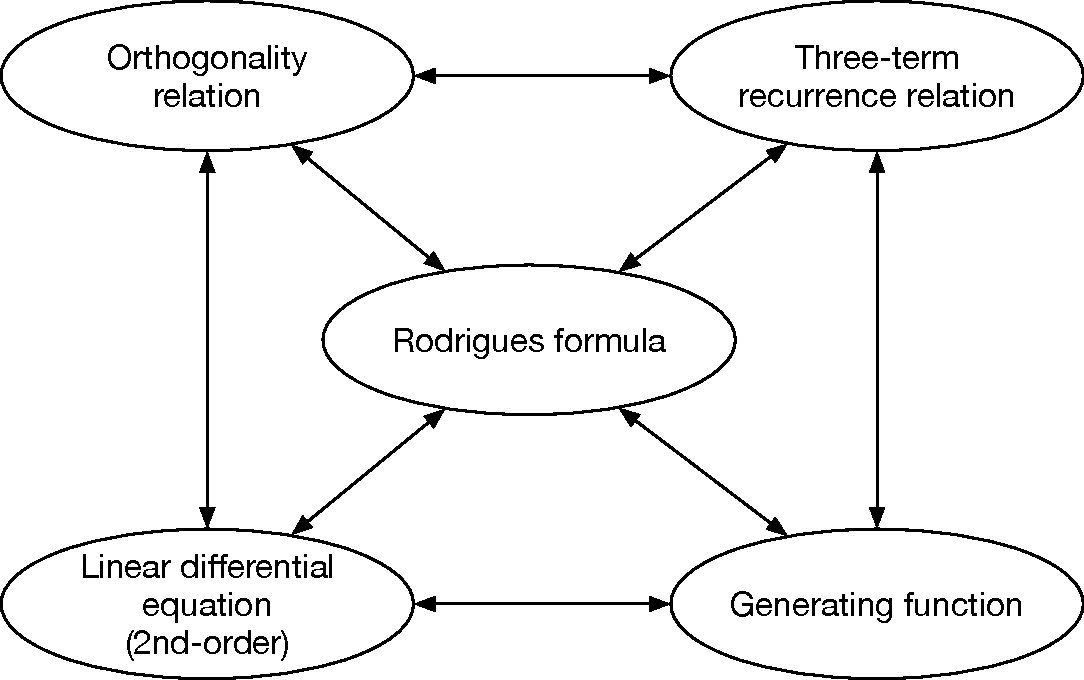
\includegraphics[width=8cm]{./Figures/20170905-poly-types-formulas}
  \label{fig:poly-classical-relations}
%
%  \small{Source: PBOC.}
\end{figure}

\subsection{埃米特多项式}
\label{sec:poly-hermite}
\begin{theorem}[埃米特多项式的罗德里格斯公式]
在区间$(-\infty,+\infty)$内,关于正态分布(normal distribution)\index{normal distribution \dotfill 正态分布} $w(x)=\exp(-x^2)$的埃米特正交多项式(Hermite polynomial)\index{polynomial!Hermite \dotfill{埃米特多项式} } $H_n(x)$,可由罗德里格斯公式予以定义(Rodrigues formula)\index{Rodrigues formula!Hermite polynomial\dotfill 罗德里格斯公式(埃米特多项式)}
\begin{equation}
  \label{eq:poly-hermite-rodrigues-formula}
  H_n(x) = \frac{(-1)^n}{w(x)} D^n w(x) = (-1)^n \exp(x^2) D^n \exp(-x^2), \quad n=0,1,2\ldots
\end{equation}
\end{theorem}
其中$(-1)^n$项是为了保证$\{D^n w(x)\}$的每一个首项系数都为正。$D=\frac{d}{d x}$是微分符,$D^n$是第$n$次求导。$D^n$遵循莱布尼兹法则(Leibniz rule)\index{Leibniz rule \dotfill 莱布尼兹法则}
\begin{equation}
  \label{eq:poly-leibniz-rule}
  D^n \left[f(x) g(x)\right] = \sum_{k=0}^{n} = \sum_{k=0}^{n} \begin{pmatrix} n \\ k \end{pmatrix} D^k f(x) D^{n-k} g(x), \quad n=0,1,2 \ldots,
\end{equation}
其中$\begin{pmatrix} n \\ k \end{pmatrix} = \frac{n!}{(n-k)!}$是帕斯卡三角(Pascal triangle identity)\index{Pascal triangle identity \dotfill 帕斯卡三角}中的二项式系数。帕斯卡三角满足关系
\begin{equation*}
  \begin{pmatrix}
    n+1 \\ k
  \end{pmatrix} = \begin{pmatrix}
    n \\ k
  \end{pmatrix} +
  \begin{pmatrix}
    n \\ k-1
  \end{pmatrix}.
\end{equation*}

帕斯卡三角的简单证明:
\begin{equation*}
\begin{split}
&  \begin{pmatrix}
    n \\ k
  \end{pmatrix} +
  \begin{pmatrix}
    n \\ k-1
  \end{pmatrix} \\
  &= \frac{n!}{k! \, (n-k)!} + \frac{n!}{(k-1)! \, (n-k+1)!}\\
  &=n! \left\{ \frac{n-k+1}{k! (n-k+1)!}  + \frac{k}{k! (n-k+1)!} \right\} \\
  &= \frac{(n+1)!}{k! (n+1-k)!} \\
  &= \begin{pmatrix}
  n+1 \\ k
  \end{pmatrix}.
\end{split}
\end{equation*}

正态分布$w(x)=\exp(-x^2)$在区间$(-3,3)$内,如图\ref{fig:poly-normal-distribution-example}所示。

\begin{figure}[htbp]
   \caption{正态分布}
  \centering
  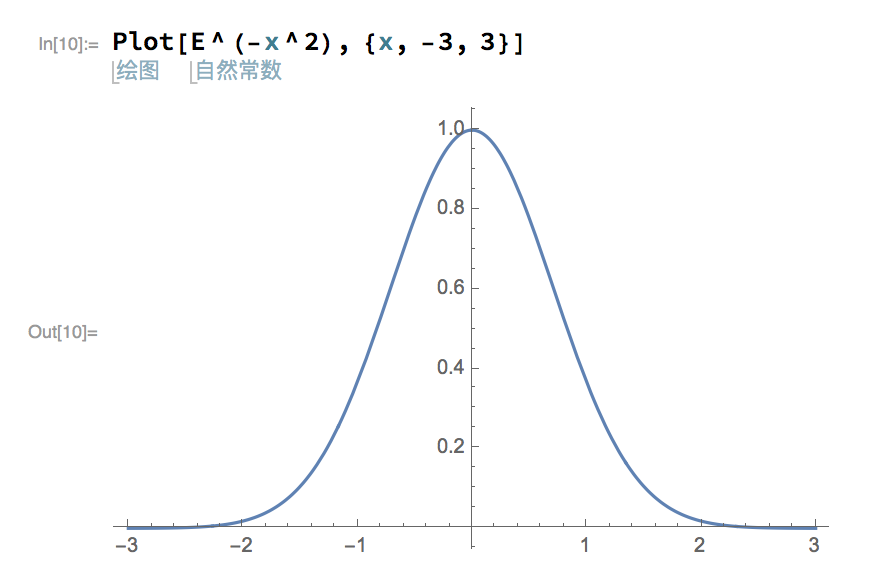
\includegraphics[width=8cm]{./Figures/20170905-normal-distri}
  \label{fig:poly-normal-distribution-example}
%

\small{$w(x) = \exp(-x^2)$在$(-3,3)$区间内的正态分布。}
\end{figure}

\begin{theorem}
  \label{theorem:poly-jacobi-poly-properties}
  由\eqref{eq:poly-hermite-rodrigues-formula}定义的埃米特多项式$H_n(x)$是一个关于$x$的$n$次多项式,并且$H_0(1)=x$,$H_n(x)$的首项系数$k_n=2^n$,$H_{2n}(x)$是偶方程,$H_{2n+1}(x)$是奇方程。
\end{theorem}
\begin{proof}
  \eqref{eq:poly-hermite-rodrigues-formula}$\Rightarrow$
  \begin{equation}
    \label{eq:poly-hermite-dnplus1}
    \begin{split}
      D^{n+1}w(x) &= D \left[D^n w(x) \right] \\
      &= D \left[ (-1)^n H_n(x) w(x) \right] \\
      &= (-1)^n \left[ w'(x) H_n(x) + w(x) H'_n(x) \right] \\
      &= (-1)^n \left[ -2x \exp(-x^2) H_n(x) + w(x) H_n(x) \right] \\
      &= (-1)^{n+1} w(x) \left[ 2x H_n(x) - H'_n(x) \right], \quad n=0,1,2 \ldots
    \end{split}
  \end{equation}

  由此,\eqref{eq:poly-hermite-rodrigues-formula}$\Rightarrow$
  \begin{equation} \label{eq:poly-hermite-diff}
        H_{n+1}(x) = \begin{cases}
        1 & n=0 \\
        \frac{(-1)^{n+1}}{w(x)} D^{n+1} w(x)=2x H_n(x)-H'_n(x) & n=1,2\ldots
        \end{cases}
  \end{equation}
\eqref{eq:poly-hermite-diff}决定了$H_n(x)$是一个$n$次多项式,并且$H_n(x)$的首项系数$k_n=2^n$,可以写出如下序列
\begin{align*}
  &p_0(x) = 1,\\
  &p_1(x) = 2x,\\
  &p_2(x) = 4x^2-2,\\
  &p_3(x) = 8x^3 - 12x,\\
  &p_4(x) = 16 x^4 - 48 x^2 + 12, \\
  &p_5(x) = 32x^5 - 160x^3 + 120x,\\
  &p_6(x) = 64 x^6 - 480 x^4 + 720 x^2 - 120,\\
  &p_7(x) = 128 x^7 - 1344 x^5 + 3360x^3 - 1680x,\\
  &\vdots
\end{align*}
由上式可得,对于偶数次$2n=2,4,6 \ldots$的情况我们有$p_{2n}(x)=p_{2n}(-x)$是偶方程;对于基数次$2n+1=1,3,5 \ldots$的情况我们有$p_{2n+1}(x)=-p_{2n}(-x)$是奇方程,如图\ref{fig:poly-hermite-examples-7-8}。

\begin{figure}[htbp]
   \caption{埃米特多项式}
  \centering
  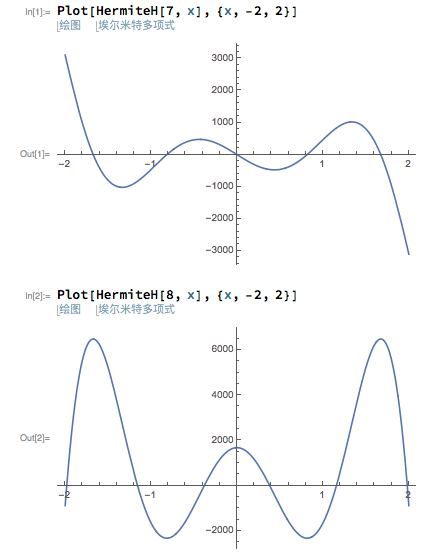
\includegraphics[width=8cm]{./Figures/20170905-hermite-examples-7-8}
  \label{fig:poly-hermite-examples-7-8}
%

\small{上图和下图分别表示$n=7,n=8$时,$H_n(x)$在$(-2,2)$区间内的值。}
\end{figure}
\end{proof}

\begin{theorem}[埃米特多项式的正交条件]
  埃米特多项式$H_n(x)$满足正交条件(orthogonality condition)\index{orthogonality condition!Hermite polynomial \dotfill 正交条件(埃米特多项式)}
  \begin{equation}
    \label{eq:poly-hermite-orthogonality-condition}
    \frac{1}{\sqrt{\pi}} \int_{-\infty}^{\infty} \exp(-x^2) H_m(x) H_n(x) \, dx = 2^n n! \delta_{mn}, \quad m,n = 0,1,2\ldots
  \end{equation}
\end{theorem}

\begin{proof}
由埃米特多项式的罗德里格斯定义式\eqref{eq:poly-hermite-rodrigues-formula}我们有,当$m<n$时
\begin{equation*}
  \begin{split}
    \int_{-\infty}^{\infty} \exp(-x^2) H_m(x) H_n(x) \, dx &= \int_{-\infty}^{\infty} \exp(-x^2) H_m(x) \left[ (-1)^n \exp(x^2) D^n \exp(-x^2) \right] \, dx \\
    &= \int_{-\infty}^{\infty} (-1)^n \exp(-x^2) H_m(x) \, dx,  \end{split}
\end{equation*}
对上式做$n$次求导,积分内的值变为零。

当$m=n$时$\Rightarrow$
\begin{equation*}
  \begin{split}
    \frac{1}{\sqrt{\pi}}  \int_{-\infty}^{\infty} \exp(-x^2) H_m(x) H_n(x) \, dx &= \frac{1}{\sqrt{\pi}} \int_{-\infty}^{\infty} \exp{(-x^2)} H_n(x) H_n(x) \, dx\\
    &=\frac{1}{\sqrt{\pi}} (-1)^n \int_{-\infty}^{\infty}  H_n(x) D^n \exp(-x^2) \, dx\\
    &=\frac{1}{\sqrt{\pi}} \int_{-\infty}^{\infty}  D^n H_n(x)  \exp(-x^2) \, dx\\
    &=\frac{k_n n!}{\sqrt{\pi}} \int_{-\infty}^{\infty} \exp (-x^2) \, dx \\
    &= k_n n!.
  \end{split}
\end{equation*}
证毕。
\end{proof}

\begin{theorem}[埃米特多项式的三项递推关系]
  埃米特多项式的三项递推关系\index{three-term recurrence relation!Hermite polynomial \dotfill 三项递推关系(埃米特多项式)}为
  \begin{equation}
    \label{poly-hermite-three-term-recurrence-relation}
    H_{n+1}(x) = 2x H_n(x) - 2n H_{n-1}(x), n=1,2,3\ldots
  \end{equation}
\end{theorem}
\begin{proof}
由正态分布$w(x)=\exp(-x^2)$我们有
\begin{equation*}
  w'(x) = -2x w(x).
\end{equation*}

代入莱布尼兹法则\eqref{eq:poly-leibniz-rule}$\Rightarrow$
\begin{equation*}
  \begin{split}
    D^{n+1}w(x) = D^n w'(x) =D^n \left[ -2x w(x) \right] = (-2x) D^n w(x) + (-2n) D^{n-1} w(x).
  \end{split}
\end{equation*}

将上式代回\eqref{eq:poly-hermite-diff}$\Rightarrow$
\begin{equation*}
  \begin{split}
    H_{n+1}(x) &= \frac{(-1)^{n+1}}{w(x)} D^{n+1}w(x)\\ %= \left[ 2xH_n(x) - H'_n(x) \right]\\
    &= (-1) \frac{(-1)^n}{w(x)} (-2x) D^n w(x) + (-1)^2  \frac{(-1)^{n-1}}{w(x)} (-2n) D^{n-1}w(x) \\
    &= \frac{(-1)^{n}}{w(x)} w(x) D^n w(x) - 2n \frac{(-1)^{n-1}}{w(x)}D^{n-1}w(x)\\
    &=2x H_n(x) - 2n H_{n-1}(x), n=1,2,3\ldots
  \end{split}
\end{equation*}
\end{proof}

\begin{theorem}[埃米特多项式的二阶线性微分方程]
  埃米特多项式的二阶线性微分方程(second order linear differential equation)\index{second order linear differential equation!Hermite polynomial \dotfill 二阶线性微分方程(埃米特多项式)}为
  \begin{equation}
    \label{eq:poly-hermite-differential-equation}
    H''_n(x) + 2n H_n(x) - 2x H'_n(x)=0.
  \end{equation}
\end{theorem}
\begin{proof}
  联立埃米特多项式的罗德里格斯公式\eqref{eq:poly-hermite-rodrigues-formula}和三项递归关系式\eqref{poly-hermite-three-term-recurrence-relation}我们有
  \begin{equation*}
  \begin{split}
    H'_n(x) = 2n H_{n-1}(x), n=1,2,3 \ldots \\
    H'_{n+1}(x) = 2(n+1) H_{n}(x), n=0,1,2 \ldots
  \end{split}
\end{equation*}

  对\eqref{eq:poly-hermite-diff}再做一次求导,并引入上式替换$H'_{n+1}(x)$我们有
  \begin{align*}
    &H'_{n+1}(x) = 2x H'_n(x) + 2 H_n(x) - H''_n(x), \\
    &\hookrightarrow 2(n+1) H_n(x) = 2x H'_n(x) + 2H_n(x) - H''(x),
  \end{align*}
这意味着$H_n(x)$构成一个二阶线性微分方程系统
\begin{equation}
  \label{eq:poly-hermite-diff-eq}
  y''(x) - 2xy'(x) + 2n y(x)=0.
\end{equation}
\end{proof}

\begin{theorem}[埃米特多项式的母方程]
  埃米特多项式的母方程(generating function)\index{generating function!Hermite polynomial \dotfill 母方程(埃米特多项式)}为
  \begin{equation}
    \label{eq:poly-hermite-generating-function}
    \exp(2xt-t^2) = \sum_{n=0}^{\infty}  \frac{H_n(x)}{n!} t^n.
  \end{equation}
\end{theorem}

\begin{proof}
  设$F(t) = \exp(-(x-t)^2) = \exp(-x^2) \exp(2xt-t^2)$. 围绕$\tilde{t}=0$对$F(t)$做泰勒级数展开近似
  \begin{equation*}
    F(t) \approx \sum_{n}^{\infty} \frac{F^{n}(0)}{n!} t^n.
  \end{equation*}

  设$u=x-t$,$\lim_{t \rightarrow 0} u \approx x$。则
  \begin{equation*}
    \begin{split}
      F^{n}(0) &= \frac{d^n}{d t^n} \exp(-(x-t)^2) = \left[ (-1)^n \frac{d^n}{d u^n} \exp(-u^2) \right]_{u=x} \\
      &=(-1)^n D^n \exp(-x^2) = \exp(-x^2) H_n(x), n=0,1,2\ldots
    \end{split}
  \end{equation*}

  $\hookrightarrow$
  \begin{equation*}
    \begin{split}
      &\exp(-x^2) \exp(-2xt-t^2) = \exp(-(x-t)^2) \\
      &= F(t) = \sum_{n=0}^{\infty} \frac{f^{(n)}(0)}{n!} t^n = \exp(-x^2) \sum_{t=0}^{\infty} \frac{H_n(x)}{n!} t^n.
    \end{split}
  \end{equation*}
\end{proof}

\subsection{拉盖尔多项式}
\label{sec:poly-laguerre}
\begin{theorem}[拉盖尔多项式的罗德里格斯公式]
在$(0,\infty)$区间内,关于伽玛分布(Gamma distribution)\index{gamma distribution \dotfill 伽玛分布} $w(x) = \exp(-x) x^{\alpha}$的拉盖尔多项式(Laguerre polynomial)\index{polynomial!Laguerre \dotfill 拉盖尔多项式} $L^{(\alpha)}_n(x)$,可由罗德里格斯公式予以定义\index{Rodrigues formula!Laguerre polynomial\dotfill 罗德里格斯公式(拉盖尔多项式)}

\begin{equation}
  \label{eq:poly-laguerre-rodrigues-formula}
  L^{(\alpha)}_n(x) = \frac{1}{n!} \frac{1}{w(x)} D^n \left[ w(x)x^n \right]= \frac{1}{n!} \exp(x) x^{-\alpha} D^n \left[ \exp(-x) x^{n+\alpha} \right], \quad n=0,1,2\ldots
\end{equation}
\end{theorem}
当$\alpha=1/2$时伽玛分布$w(x) = \exp (-x) x^{\alpha}$在区间$(-3,3)$内,如图\ref{fig:poly-gamma-distribution-example}所示。

\begin{figure}[htbp]
   \caption{伽玛分布}
  \centering
  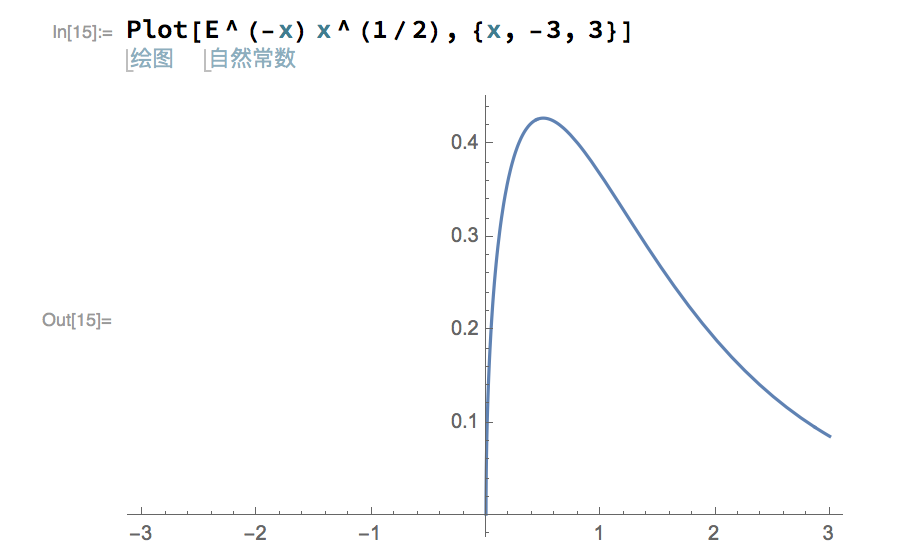
\includegraphics[width=8cm]{./Figures/20170906-gamma-distri}
  \label{fig:poly-gamma-distribution-example}
%

\small{$w(x) = \exp(-x) x^{\alpha}$在$(-3,3)$区间内的正态分布$(\alpha = 1/2)$。}
\end{figure}

\begin{theorem}
  拉盖尔多项式$L^{(n)}(x)$是一个关于$x$的$n$次多项式。$L^{(\alpha)}(0) = \frac{(\alpha+1)_n}{n!}$,$L^{(n)}(x)$的首项系数$k_n = \frac{(-1)^n}{n!}$。
\end{theorem}
\begin{proof}
  根据莱布尼兹法则\eqref{eq:poly-leibniz-rule}我们有
  \begin{equation*}
    \begin{split}
      D^n \left[ \exp(-x) x^{n+\alpha} \right] &= \sum_{k=0}^n \begin{pmatrix} n \\ k \end{pmatrix} D^k \exp(-x) D^{n-k} x^{n+\alpha} \\
      &= \sum_{k=0}^{n} \begin{pmatrix} n \\ k \end{pmatrix} (-1)^k \exp(-x) x^{\alpha + k }(n+\alpha)(n+\alpha-1) \ldots (n + k + 1) \\
      &= \exp(-x) x^{\alpha}  \sum_{k=0}^{n} (-1)^k \begin{pmatrix} n \\ k \end{pmatrix} \frac{\Gamma (n+\alpha + 1)}{\Gamma (k + \alpha + 1)} x^k.
    \end{split}
  \end{equation*}
最后一个等式的简单数学计算:
\begin{equation*}
  \begin{split}
    \frac{\Gamma (n+\alpha + 1)}{\Gamma (k + \alpha + 1)} &= \frac{
    \int_0^{\infty} \exp(-t) t^{n+\alpha} \, dt
    }{
    \int_0^{\infty} \exp(-t) t^{k+\alpha} \, dt
    } \approx \frac{(n+\alpha)!}{(k+\alpha)!}
  \end{split}
\end{equation*}

因此我们有
\begin{equation}
  \label{eq:poly-laguerre-def-intermediate}
  L_n^{(\alpha)}(x) = \sum_{k=0}^n (-1)^k \begin{pmatrix} n+\alpha \\ n-k \end{pmatrix} \frac{x^k}{k!}, \quad \text{其中} \begin{pmatrix} n+\alpha \\ n-k \end{pmatrix} = \frac{\Gamma (n+\alpha + 1)}{\Gamma (k + \alpha + 1)}(n-k)!
\end{equation}
由上式可见,$L^{(\alpha)}_n(x)$是一个$n$次多项式。此外,由于
\begin{equation*}
  (-1)^k \begin{pmatrix} n+\alpha \\ n-k \end{pmatrix} = \frac{(-1)^k}{(n-k)!}\frac{(n+\alpha)!}{(\alpha + k)!} = \frac{(-1)^k}{(n-k)!} \frac{(\alpha +1)_n}{(\alpha+1)_k} = \frac{(\alpha+1)_n}{n!} \frac{(-n)_k}{(\alpha+1)_k},
\end{equation*}
我们可得拉盖尔多项式的超几何方程\index{hypergeometric function!Laguerre polynomial \dotfill 超几何方程(拉盖尔多项式)}
\begin{equation}
  \label{eq:poly-laguerre-hgf}
  L_n^{(\alpha)}(x) = \frac{(\alpha+1)_n}{n!} \sum_{k=0}^{n} \frac{(-n)_k}{(\alpha+1)_k} \frac{x^k}{k!} = \begin{pmatrix}
  n+\alpha \\ n
\end{pmatrix}\pFq{1}{1}{-n}{\alpha+1}{x}.
\end{equation}

由\eqref{eq:poly-laguerre-hgf}得$x=0$时
\begin{equation*}
  L^{(\alpha)}_n(0) = \begin{pmatrix} n+\alpha \\ n \end{pmatrix} = \frac{(\alpha+1)_n}{n!}, \quad n=0,1,2\ldots
\end{equation*}
$\hookrightarrow$
\begin{equation*}
  k_n = \frac{(-1)^n}{n!}, \quad n=0,1,2\ldots
\end{equation*}
\end{proof}

\begin{theorem}[拉盖尔多项式的正交条件]
  拉盖尔多项式$L^{(\alpha)}_n(x)$的正交条件\index{orthogonality condition!Laguerre polynomial \dotfill 正交条件(拉盖尔多项式)}满足
  \begin{equation}
    \label{eq:poly-laguerre-poly-orghogonality-condition}
    \int_0^{\infty} \exp(-x) x^{\alpha} L_m^{(\alpha)}(x) L_n^{(\alpha)}(x) \, dx = \frac{\Gamma(n+\alpha+1)}{n!} \delta_{mn}, \alpha > -1.
  \end{equation}
\end{theorem}
\begin{proof}
  定义矩
\begin{equation*}
  \mu_n := \int_0^{n} \exp(-x) x^{n+\alpha} \, dx,
\end{equation*}
如果对于所有$n=0,1,2\ldots$,$\mu_n$都存在,那么\eqref{eq:poly-laguerre-poly-orghogonality-condition}的LHS积分是收敛的,因此需要$\alpha > -1$\todo{这部分还需要做进一步的说明。}。此外根据定义我们有
\begin{equation*}
  \mu_n = \Gamma (n+\alpha + 1).
\end{equation*}

进而,由拉盖尔多项式的罗德里格斯公式\eqref{eq:poly-laguerre-rodrigues-formula}我们有

\begin{equation*}
  \begin{split}
    &\int_0^{\infty} \exp(-x) x^{\alpha} L_m^{(\alpha)}(x) L_n^{(\alpha)}(x) \, dx
    \\&= \int_0^{\infty} \exp(-x) x^{\alpha} L_m^{(\alpha)}(x) \left\{
    \frac{1}{n!} \exp(-x) x^{\alpha} D^n \left[ \exp(-x) x^{n+\alpha} \right]
    \right\} \, dx \\
    &= \frac{-1}{n!} \int_0^{\infty} L_m^{(\alpha)} (x) D^n \left[ \exp(-x) x^{n+\alpha}  \right] \, dx \\
    &= \frac{(-1)^n}{n!} \int_0^{\infty} L_m^{(\alpha)} (x) D^n \left[ \exp(-x) x^{n+\alpha}  \right] \, dx
  \end{split}
\end{equation*}
当$m<n$时,对上式做$n$次求导,积分内的值变为零。当$m=n$时 $\Rightarrow$
\begin{equation*}
  \begin{split}
    &\frac{(-1)^n}{n!} \int_0^{\infty} L_m^{(\alpha)} (x) D^n \left[ \exp(-x) x^{n+\alpha}  \right] \, dx \\
    &= \frac{(-1)^n}{n!} k_n n! \int_0^{\infty} \exp(-x) x^{n+\alpha} \, dx \\
    &= \frac{\Gamma (n+\alpha + 1)}{n!}.
  \end{split}
\end{equation*}
\end{proof}

\begin{theorem}[拉盖尔多项式的母方程]
  拉盖尔多项式$L_n^{(\alpha)}(x)$的母方程\index{generating function!Laguerre polynomial \dotfill 母方程(拉盖尔多项式)}为
  \begin{equation}
    \label{eq:poly-laguerre-generating-function-def}
    (1-t)^{-\alpha - 1} \exp \left( - x \frac{t}{1-t} \right) = \sum_{n=0}^{\infty} L_n^{(\alpha)}(x) t^n.
  \end{equation}
\end{theorem}
\begin{proof}
将\eqref{eq:poly-laguerre-hgf}代入\eqref{eq:poly-laguerre-generating-function-def}RHS $\Rightarrow$
\begin{equation*}
  \begin{split}
    &\sum_{n=0}^{\infty} L_n^{(\alpha)}(x) t^n \\
    &=\sum_{n=0}^{\infty} \frac{(\alpha+1)_n}{n!} t^n \sum_{k=0}^{n} \frac{
    (-n)_k
    }{
    (\alpha + 1)_k
    } \frac{
    x^k
    }{k!}\\
    &=\sum_{k=0}^{\infty} \sum_{n=0}^{\infty} \frac{(\alpha+1)_n}{(\alpha+1)_k} \frac{
    (-1)^k x^k t^n
    }{
    k! (n-k)!
    } \\
    &=\sum_{k=0}^{\infty} \sum_{n=0}^{\infty}
    \frac{(\alpha+1)_{n+k}}{(\alpha+1)_k}
    \frac{(-1)^k x^k t^{n+k}}{k! n!}\\
    &= \sum_{k=0}^{\infty} \frac{(- x t)^k}{k!}
    \sum_{n=0}^{\infty} \frac{(\alpha + k + 1)_n}{n!} t^n \\
    &=\sum_{k=0}^{\infty} \frac{(-xt)^k}{k!} (1-t)^{(-\alpha - k - 1)}\\
    &=(1-t)^{-\alpha -1} \sum_{k=0}^{\infty} \frac{1}{k!} \left(- x \frac{t}{1-t} \right)^{k}\\
    &=(1-t)^{-\alpha - 1} \exp \left( - x \frac{t}{1-t} \right).
  \end{split}
\end{equation*}
\end{proof}

\begin{theorem}
  由拉盖尔多项式的母方程\eqref{eq:poly-laguerre-generating-function-def}我们有
  \begin{equation}
    L_n^{(\alpha + \beta + 1)}(x + y) = \sum_{k=0}^{n} L_{k}^{(\alpha)} (x) L_{n-k}^{(\beta)} (y).
  \end{equation}
\end{theorem}
\begin{proof}
  \eqref{eq:poly-laguerre-generating-function-def}$\Rightarrow$
  \begin{equation*}
    \begin{split}
    \sum_{n=0}^{\infty}  L_n^{(\alpha + \beta + 1)} (x + y) t^n &= (1-t)^{- \alpha - \beta -2} \exp \left[ - (x+y)\frac{t}{1-t}\right] \\
    &= \left[ (1-t)^{-\alpha -1} \exp \left( -x \frac{t}{1-t} \right) \right] \left[ (1-t)^{(-\beta - 1)} \exp \left(-y \frac{1}{1-t} \right) \right]\\
    &=\left[ \sum_{k=0}^{\infty} L_{k}^{(\alpha)} (x) t^k \right] \left[ \sum_{m=0}^{\infty} L_{m}^{(\beta)} (y) t^m\right] \\
    &=\sum_{n=0}^{\infty} \left[ \sum_{k=0}^{n} L_{k}^{(\alpha)}(x) L_{n-k}^{(\beta)}(y) \right] t^n.
    \end{split}
  \end{equation*}
  证毕。
\end{proof}

\begin{theorem}[拉盖尔多项式的三项递推关系]
  拉盖尔多项式$L_n^{(\alpha)}(x)$的三项递推关系\index{three-term recurrence relation!Laguerre polynomial \dotfill 三项递推关系(拉盖尔多项式)}为
  \begin{equation}
    \label{eq:poly-laguerre-three-term-recurrence-relation}
    (n+1) L_{n+1}^{(\alpha)}(x) + (x - 2n - \alpha - 1) L_{n}^{(\alpha)}(x) + (n+\alpha) L_{n-1}^{(\alpha)}(x) =0, \quad n = 1,2,3\ldots
  \end{equation}
\end{theorem}

\begin{proof}

首先由\eqref{eq:poly-laguerre-def-intermediate}得
\begin{equation}
  \label{eq:poly-laguerre-diff-x}
\begin{split}
    \frac{d}{dx} L_n^{(\alpha)}(x) &= \frac{d}{dx} \sum_{k=0}^{n} (-1)^k \begin{pmatrix}
    n+\alpha \\ n-k
  \end{pmatrix} \frac{x^k}{k!}\\
  &=\sum_{k=1}^{n} (-1)^k \begin{pmatrix}
  n+\alpha \\ n-k
\end{pmatrix}  \frac{x^{k-1}}{(k-1)!} \\
&= \sum_{k=0}^{n-1} (-1)^{k-1} \begin{pmatrix}
n+\alpha \\ n-k-1
\end{pmatrix}  \frac{x^{k}}{(k)!}\\
&= - L_{n-1}^{(\alpha + 1)}(x), n=1,2,3\ldots
\end{split}
\end{equation}
为简化表述,根据拉盖尔多项式的母方程\eqref{eq:poly-laguerre-generating-function-def},定义
\begin{equation*}
  F(x,t) := (1-t)^{-\alpha - 1} \exp \left( - x \frac{t}{1-t} \right) = \sum_{n=0}^{\infty} L_n^{(\alpha)}(x) t^n.
\end{equation*}

则我们有第一个偏导数
\begin{equation}
  \label{eq:poly-laguerre-three-partial-f-x}
  \begin{split}
    &\frac{\partial F(x,t)}{\partial x} = (-t) (1-t)^{-\alpha - 2} \exp \left( - x \frac{t}{1-t} \right), \\
    &\Rightarrow (1-t) \frac{\partial F(x,t)}{\partial x} + t F(x,t) = 0,\\
    &\Rightarrow (1-t) \sum_{n=0}^{\infty} \frac{d}{dx} L_n^{(\alpha)}(x) t^n + t \sum_{n=0}^{\infty} L_n^{(\alpha)} (x) t^n = 0, \\
    & \Rightarrow \underbrace{\sum_{n=0}^{\infty} \frac{d}{dx} L_n^{(\alpha)}(x) t^n}_{n\rightarrow n+1} - \sum_{n=0}^{\infty} \frac{d}{dx} L_n^{(\alpha)}(x) t^{n+1} + \sum_{n=0}^{\infty} L_n^{(\alpha)} (x) t^n = 0,\\
    & \Rightarrow \frac{d}{dx} L_{n+1}^{(\alpha)}(x)
    - \frac{d}{dx} L_n^{(\alpha)}(x)
    + L_n^{(\alpha)} (x)= 0,
  \end{split}
\end{equation}

上式代入\eqref{eq:poly-laguerre-diff-x}有
\begin{equation*}
\begin{split}
  &-L_n^{(\alpha+1)}(x) - \frac{d}{dx}L_n^{(\alpha)}(x) + L_n^{(\alpha)}(x)=0, \\
  &\Rightarrow \frac{d}{dx}L_n^{(\alpha)}(x) = L_n^{(\alpha)}(x) - L_n^{(\alpha+1)}(x), \quad n = 0,1,2\ldots
\end{split}
\end{equation*}

第二个偏导数
\begin{equation*}
\begin{split}
  &\frac{\partial F(x,t)}{\partial t} =
  \left[ (\alpha + 1) (1-t)^{-\alpha - 2} + (1-t)^{-\alpha - 1} \frac{-x(1-t)-xt}{(1-t)^2} \right] \exp \left( - x \frac{t}{1-t} \right) \\
  &=\left(\alpha + 1 - \frac{x}{1-t} \right) (1-t)^{-\alpha - 2} \exp \left( - x \frac{t}{1-t} \right), \\
  &\Rightarrow (1-t)^2 \frac{\partial F(x,t)}{\partial t} + \left[ x - (\alpha - 1)(1-t) \right] F(x,t) = 0,\\
  &\Rightarrow (1-t)^2 \sum_{n=1} n L_n^{(\alpha)} (x) t^{(n-1)} + \left[ x - (\alpha + 1) (1-t) \right] \sum_{n=0}^{\infty} L_n^{\alpha} (x) t^n = 0,
  \end{split}
\end{equation*}
将各项拆出
\begin{equation*}
  \begin{split}
    &\sum_{n=1}^{\infty} n L_{n}^{\alpha}(x) t^{n-1}
    -2 \sum_{n=1}^{\infty} n L_{n}^{\alpha}(x) t^n
    + \sum_{n=1}^{\infty} n L_{n}^{\alpha}(x) t^{n+1} \\
    &+ x \sum_{n=0}^{\infty} L_{n}^{\alpha}(x) t^n
    + (\alpha + 1) \sum_{n=0}^{\infty} L_{n}^{\alpha}(x) t^{n+1}
    -(\alpha+1) \sum_{n=0}^{\infty} L_{n}^{\alpha}(x) t^n = 0,
  \end{split}
\end{equation*}

按照$t$的幂次重新排列组合,得三项递推关系式\eqref{eq:poly-laguerre-three-term-recurrence-relation}。
\end{proof}

\begin{theorem}[拉盖尔多项式的二阶线性微分方程]
  拉盖尔多项式$L_n^{(\alpha)}(x)$的二阶线性微分方程\index{second order linear differential equation!Laguerre polynomial \dotfill 二阶线性微分方程(拉盖尔多项式)}为
  \begin{equation*}
    \label{eq:poly-laguerre-linear-diff-equation}
    x \frac{d^2}{d x^2}L_n^{(\alpha)}(x)+ \left( \alpha + 1 - x \right) \frac{d}{dx}L_n^{(\alpha)}(x) + n  L_n^{(\alpha)}(x) = 0.
  \end{equation*}
\end{theorem}
\begin{proof}
  拉盖尔多项式的三项递推关系\eqref{eq:poly-laguerre-three-term-recurrence-relation}$\Rightarrow$
  \begin{equation*}
    x L_n^{(\alpha)}(x) + (n+1) \left[ L_{n+1}^{(\alpha)}(x) - L_n^{(\alpha)}(x)\right] - (n + \alpha)  \left[ \frac{d}{dx}L_n^{(\alpha)}(x) -  \frac{d}{dx}L_{n-1}^{(\alpha)}(x) \right]=0.
  \end{equation*}

对$x$求导$\Rightarrow$
\begin{equation*}
  \begin{split}
    L_n^{(\alpha)} (x) + x \frac{d}{dx} L_n^{(\alpha)} (x) + (n+1) \frac{d}{dx} L_{n+1}^{(\alpha)} (x) - (n+1) \frac{d}{dx} L_{n}^{(\alpha)} (x) - (n+\alpha) \frac{d}{dx} L_{n}^{(\alpha)} (x) + (n+\alpha) \frac{d}{dx} L_{n-1}^{(\alpha)} (x) = 0,
  \end{split}
\end{equation*}
引入\eqref{eq:poly-laguerre-three-partial-f-x}替换上式中的$\frac{d}{dx}L_{n+1}^{(\alpha)}(x)$和$\frac{d}{dx}L_{n}^{(\alpha)}(x)$
  \begin{align}
    &L_n^{(\alpha)} (x)+ x \frac{d}{dx} L_n^{(\alpha)} (x) - (n+1) L_n^{(\alpha)} (x) + (n+\alpha) L_{n-1}^{(\alpha)} (x) = 0, \nonumber \\
    \label{eq:poly-laguerre-first-order-diff}
    &x \frac{d}{dx} L_n^{(\alpha)} (x) = n L_n^{(\alpha)} (x) - (n+\alpha) L_{n-1}^{(\alpha)} (x).
  \end{align}
  上式继续对$x$求导$\Rightarrow$
  \begin{equation}
    \label{eq:poly-laguerre-second-order-diff}
      \begin{split}
        \frac{d}{dx} L_n^{(\alpha)} (x) + x \frac{d^2}{dx^2} L_n^{(\alpha)} (x) &= n \frac{d}{dx} L_n^{(\alpha)} (x) -(n+\alpha) \frac{d}{dx} L_{n-1}^{(\alpha)} (x) \\
        &= (n+\alpha) \left( \frac{d}{dx} L_n^{(\alpha)} (x)- \frac{d}{dx} L_{n-1}^{(\alpha)} (x) \right) - \alpha \frac{d}{dx} L_n^{(\alpha)} (x) \\
        &= -(n+\alpha) L_{n-1}^{(\alpha)} (x) - \alpha \frac{d}{dx} L_n^{(\alpha)} (x) \\
        &= x \frac{d}{dx}L_n^{(\alpha)} (x) - n L_n^{(\alpha)} (x) - \alpha \frac{d}{dx}L_n^{(\alpha)} (x),
      \end{split}
  \end{equation}
  $\hookrightarrow$
  \begin{equation*}
    \begin{split}
      \frac{d^2}{dx^2} L_n^{(\alpha)}(x) + (1 + \alpha - x) \frac{d}{dx} L_n^{(\alpha)}(x) + n L_n^{(\alpha)}(x) = 0, \\
      \Rightarrow xy''(x) + (1 + \alpha - x) y'(x) + n y(x) =0, \quad n=0,1,2\ldots
    \end{split}
  \end{equation*}
\end{proof}

\subsection{雅各比多项式}
\label{sec:poly-jacobi-polynomial}
\begin{theorem}[雅各比多项式的罗德里格斯公式]
在$(-1,1)$区间内,关于贝塔分布(Beta distribution)\index{Beta distribution \dotfill 贝塔分布} $w(x)=(1-x)^{\alpha} (1+x)^{\beta}$的雅各比多项式(Jacobi polynomial)\index{polynomial!Jacobi \dotfill 雅各比多项式} $P_n^{(\alpha,\beta)}(x)$ ,可由罗德里格斯公式\index{Rodrigues formula!Jacoby polynomial \dotfill 罗德里格斯公式(雅各比多项式)}予以定义
\begin{equation}
  \label{eq:poly-jacobi-polynomial-def}
  \begin{split}
    P_n^{(\alpha,\beta)} (x) &= \frac{(-1)^n}{2^n n!} \frac{1}{w(x)} D^n \left[ w(x) (1-x^2)^n \right] \\
    &= \frac{(-1)^n}{2^n n!} (1-x)^{-\alpha} (1+x)^{-\beta} D^n \left[ (1-x)^{n+\alpha} (1+x)^{n+\beta} \right], \quad \alpha, \beta > -1, n=0,1,2\ldots
  \end{split}
\end{equation}
\end{theorem}

当$(\alpha,\beta)=(3,2)$时贝塔分布$w(x)=(1-x)^{\alpha} (1+x)^{\beta}$在区间$(-2,2)$内,如图\ref{fig:poly-beta-distribution-example}所示。

\begin{figure}[htbp]
   \caption{贝塔分布}
  \centering
  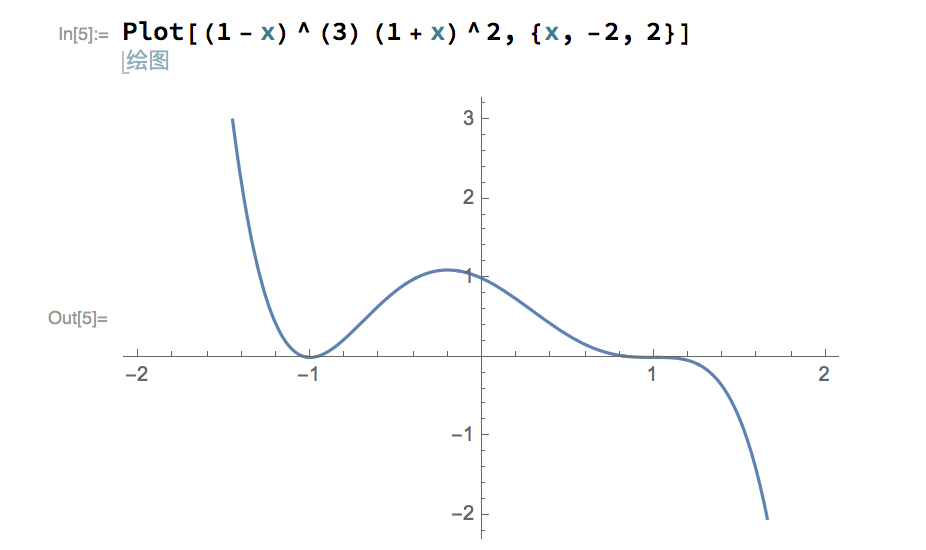
\includegraphics[width=8cm]{./Figures/20170906-beta-distri}
  \label{fig:poly-beta-distribution-example}
%

\small{$w(x)=(1-x)^{\alpha} (1+x)^{\beta}$在$(-2,2)$区间内的正态分布$(\alpha = 3, \beta = 2)$。}
\end{figure}

\begin{theorem}
  \label{theorem:poly-jacobi-properties}
  雅各比多项式$P_n^{(\alpha,\beta)}(x)$是一个关于$x$的$n$次多项式。$P_n^{(\alpha,\beta)}(x)$是奇方程,并且$P_n^{(\alpha,\beta)}(1) = \begin{pmatrix} n+\alpha \\ n \end{pmatrix}$, $P_n^{(\alpha,\beta)}(-1) = (-1)^n \begin{pmatrix} n+\beta \\ n \end{pmatrix}, \quad n=0,1,2\ldots$
\end{theorem}
\begin{proof}
  根据莱布尼兹法则\eqref{eq:poly-leibniz-rule}我们有
  \begin{equation*}
    \begin{split}
      &D^n \left[  (1-x)^{n+\alpha} (1+x)^{n+\beta} \right] \\
      &= \sum_{k=0}^{n} \begin{pmatrix}
      n \\ k
      \end{pmatrix}
      D^k (1-x)^{n+\alpha} D^{n-k} (1+x)^{n+\beta} \\
      &=\sum_{k=0}^{n} \begin{pmatrix}
      n \\ k
      \end{pmatrix} (-1)^k
      (n+\alpha) (n+\alpha-1) (n+\alpha-2) \ldots (n+\alpha-k+1) (1-x)^{n+\alpha-k} \\
      &\qquad \times  (n+\beta) (n+\beta-1) (n+\beta-2) \ldots (\beta+k+1) (1+x)^{\beta+k} \\
      &=n! \sum_{k=0}^{n} (-1)^k \begin{pmatrix}
      n+\alpha \\ k
      \end{pmatrix}
      \begin{pmatrix}
        n+\beta \\ n-k
      \end{pmatrix}
      (1-x)^{n+\alpha - k} (1+x)^{\beta + k}, \quad n=0,1,2\ldots
    \end{split}
  \end{equation*}

代回\eqref{eq:poly-jacobi-polynomial-def}$\Rightarrow$
\begin{equation}
  \label{eq:poly-jacobi-poly-degree-n}
  \begin{split}
    P_n^{(\alpha,\beta)} (x) &= \frac{(-1)^n}{2^n n!} (1-x)^{-\alpha} (1+x)^{-\beta} D^n \left[ (1-x)^{n+\alpha} (1+x)^{n+\beta} \right] \\
    &= \frac{(-1)^n}{2^n} \sum_{k=0}^{n} (-1)^k \begin{pmatrix}
    n+\alpha \\ k
    \end{pmatrix}
    \begin{pmatrix}
      n+\beta \\ n-k
    \end{pmatrix}
    (1-x)^{n- k} (1+x)^k, \quad n=0,1,2\ldots
  \end{split}
\end{equation}

这表明雅各比多项式$P_n^{(\alpha,\beta)}(x)$是一个关于$x$的$n$次多项式。

\eqref{eq:poly-jacobi-polynomial-def} $\Rightarrow$ $P_n^{(\alpha,\beta)}(x)$的对称性(略):
\begin{equation}
  \label{eq:poly-jacobi-symmetry}
  P_n^{(\alpha,\beta)}(-x) = (-1)^n P_n^{(\alpha,\beta)}(x), \quad n=0,1,2 \ldots
\end{equation}

\eqref{eq:poly-jacobi-polynomial-def} $\Rightarrow$
\begin{align*}
  &P_n^{(\alpha,\beta)}(1) = \frac{(-1)^n}{2^n} \sum_{k=0}^{n} (-1)^k \frac{(n+\alpha)!}{(n+\alpha-k)! \, k!}\frac{(n+\beta)!}{(n+\beta+k)! \, (n-k)!} (1+x)^k = \begin{pmatrix}
  n+\alpha \\ n
  \end{pmatrix},\\
  & P_n^{(\alpha,\beta)}(-1) = (-1)^n \begin{pmatrix}
  n+\beta \\ n
  \end{pmatrix}.
\end{align*}
\end{proof}

\begin{theorem}[雅各比多项式的超几何方程]
  \label{theorem:poly-jacobi-hgf}
雅各比多项式的$P_n^{(\alpha,\beta)}(x)$的超几何方程\index{hypergeometric function!Jacobi polynomial \dotfill 超几何方程(雅各比多项式)}可表示为
\begin{equation}
  \label{eq:poly-jacobi-hypergeometric-function}
  P_{n}^{(\alpha, \beta)}(x) = \begin{pmatrix}
  n+\alpha \\ n
  \end{pmatrix}
  \pFq{2}{1}{-n,n+\alpha+\beta+1}{\alpha+1}{\frac{1-x}{2}}, \quad n=0,1,2\ldots
\end{equation}
\end{theorem}
\begin{proof}
  对于$x \neq 1$的情况,  \eqref{eq:poly-jacobi-poly-degree-n}$\Rightarrow$
  \begin{equation*}
    P_n^{(\alpha,\beta)}(x) = \left(\frac{x-1}{2}\right)^n \sum_{k=0}^{\infty} \begin{pmatrix}
    n+\alpha \\ n
    \end{pmatrix}
    \begin{pmatrix}
      n+\beta \\ n-k
    \end{pmatrix}
    \underbrace{\left( \frac{x+1}{x-1} \right)^k}, \quad n=0,1,2\ldots
  \end{equation*}
其中
\begin{equation}
  \label{eq:poly-jacobi-hgf-intermediate}
  \begin{split}
    \left( \frac{x+1}{x-1} \right)^k &= \left( 1 + \frac{2}{x-1} \right)^k, \quad k=0,1,2 \ldots \\
    &= \sum_{i=0}^{k} \begin{pmatrix}
    k \\ i
    \end{pmatrix}
    \left( \frac{2}{x-1} \right)^i \\
    &=  \left( \frac{2}{x-1} \right)^{n} \sum_{i=0}^{n} \sum_{k=i}^{n}
    \begin{pmatrix}
    n+\alpha \\ k
    \end{pmatrix}
    \begin{pmatrix}
    n+\beta \\ n-k
    \end{pmatrix}
    \begin{pmatrix}
    k \\ i
    \end{pmatrix}
     \left( \frac{2}{x-1} \right)^{i} \\
     &= \left( \frac{2}{x-1} \right)^{n} \sum_{i=0}^{n}\sum_{k=0}^{n-i}
     \begin{pmatrix}
      n+ \alpha \\ i+k
     \end{pmatrix}
     \begin{pmatrix}
      n+ \beta \\ n-i-k
     \end{pmatrix}
     \begin{pmatrix}
      i+k \\ k
     \end{pmatrix}
     \left( \frac{2}{x-1} \right)^{i}\\
     &=\left( \frac{2}{x-1} \right)^{n}  \sum_{i=0}^{n}\sum_{k=0}^{n}
     \begin{pmatrix}
      n+ \alpha \\ n-i+k
     \end{pmatrix}
     \begin{pmatrix}
      n+ \beta \\ i-k
     \end{pmatrix}
     \begin{pmatrix}
      n-i+k \\ n-i
     \end{pmatrix}
     \left( \frac{2}{x-1} \right)^{i}\\
     &=\sum_{i=0}^{n}\sum_{k=0}^{n}
     \begin{pmatrix}
      n+ \alpha \\ n-i+k
     \end{pmatrix}
     \begin{pmatrix}
      n+ \beta \\ i-k
     \end{pmatrix}
     \begin{pmatrix}
      n-i+k \\ n-i
     \end{pmatrix}
     \left( \frac{2}{x-1} \right)^{i}\\
     &= \sum_{i=0}^{n}\sum_{k=0}^{n} \frac{
     \Gamma (n+\alpha + 1)
     }{
     (n-i+k)! \, \Gamma(i-k+\alpha +1)
     }
     \frac{
     \Gamma(n+\beta+1)
     }{
     (i-k)! \, \Gamma(n-i+k+\beta+1)
     }
     \frac{
     (n-i+k)!
     }{
     (n-i)! \, k!
     }
     \left( \frac{x-1}{2} \right)^i \\
     &=\frac{
     \Gamma(n+\alpha + 1) \, \Gamma(n+\beta + 1)
     }{n!}
     \sum_{i=0}^{n}
     \frac{
     (-n)_{i}
     }{
     \Gamma(i + \alpha + 1) \, \underbrace{\Gamma(n-i+\beta + 1)}
     }
     \left( \frac{2}{x-1} \right)^{i} \\
     &\qquad \underbrace{\sum_{k=0}^n \frac{
     (-i)_k \, (-i - \alpha - 1)_k
     }{
     (n-i+\beta+1)_k \, k!
     }},
  \end{split}
\end{equation}
其中,首先根据朱世杰——范德蒙德求和公式\index{Chu-Vandermonde summation \dotfill 朱世杰——范德蒙德求和公式}我们有
\begin{equation*}
  \sum_{k=0}^n \frac{
  (-i)_k \, (-i - \alpha - 1)_k
  }{
  (n-i+\beta+1)_k \, k!
  } = \pFq{2}{1}{-i,-i-\alpha-1}{n-i+\beta+1}{1}=\frac{
  (n+\alpha+\beta+1)_{i}
  }{
  (n-i+\beta+1)_{i}
  },
\end{equation*}
其次
\begin{equation*}
  \Gamma(n-i+\beta + 1) (n-i+\beta+1)_i = \Gamma(n+\beta+1),
\end{equation*}
因此\eqref{eq:poly-jacobi-hgf-intermediate}进一步改写为
\begin{equation}
  \label{eq:poly-jacobi-hgf}
\begin{split}
  P_n^{(\alpha,\beta)}(x) &= \frac{\Gamma(n+\alpha+1)}{n!} \sum_{i=0}^n \frac{
  (-n)_i \, (n+\alpha+\beta+1)_i
  }{
  \Gamma(i+\alpha+1) \, i!
  }
  \left( \frac{1-x}{2} \right)^i \\
  &= \frac{\Gamma(n+\alpha+1)}{\Gamma(\alpha+1) \, n!} \sum_{i=0}^n \frac{
  (-n)_i \, (n+\alpha+\beta+1)_i
  }{
  (\alpha + 1)_i i!
  }
  \left( \frac{1-x}{2} \right)^i \\
  &= \begin{pmatrix}
  n+\alpha \\ n
  \end{pmatrix}
  \pFq{2}{1}{-n, n+\alpha+\beta+1}{\alpha+1}{\frac{1-x}{2}}, \quad n=0,1,2\ldots
\end{split}
\end{equation}

此外由奇函数的对称性质\eqref{eq:poly-jacobi-symmetry}我们有
\begin{equation*}
  P_{n}^{(\alpha,\beta)}(-x) = (-1)^n \begin{pmatrix}
  n+\beta \\ n
  \end{pmatrix}
  \pFq{2}{1}{-n, n+\alpha+\beta+1}{\beta+1}{\frac{1+x}{2}}, \quad n=0,1,2\ldots
\end{equation*}
\end{proof}

\begin{theorem}[雅各比多项式的首项系数]
    雅各比多项式$P_n^{(\alpha,\beta)}(x)$的首项系数$k_n$为
    \begin{equation}
      \label{eq:poly-jacobi-leading-coeff-n}
      k_n = \frac{n+\alpha+\beta+1}{2^n \, n!}, \quad n=0,1,2 \ldots
    \end{equation}
\end{theorem}
\begin{proof}
  由雅各比多项式的超几何方程\eqref{eq:poly-jacobi-hgf}得
  \begin{equation*}
      k_n = \begin{pmatrix}
      n+\alpha \\ n
      \end{pmatrix}
      \frac{
      (-n)_n \, (n+\alpha+\beta+1)_n
      }{
      (\alpha+1)_n \, n!
      }
      \frac{
      (-1)^n
      }{
      2^n
      }
      =\frac{n+\alpha+\beta+1}{2^n \, n!}, \quad n=0,1,2 \ldots
  \end{equation*}
\end{proof}

\begin{theorem}[雅各比多项式的正交条件]
  雅各比多项式$P_n^{(\alpha,\beta)}(x)$满足如下正交关系\index{orthogonality condition!Jacobi polynomial \dotfill 正交条件(雅各比多项式)}
  \begin{equation}
    \label{eq:poly-jacobi-orthogonality-relation}
    \begin{split}
      &\int_{-1}^{1} (1-x)^{\alpha} (1+x)^{\beta} P_m^{(\alpha,\beta)}(x) P_n^{(\alpha,\beta)}(x) \, dx = \frac{
      2^{\alpha + \beta + 1} \, \Gamma(n+\alpha+1) \, \Gamma (n + \beta + 1)
      }{
      \left( 2n + \alpha + \beta + 1 \right) \, \Gamma(n+\alpha+\beta+1) \, n!
      } \delta_{mn}, \\
      & \qquad \text{for} \, \alpha > -1, \beta > -1, m,n \in \{0,1,2\ldots\}
    \end{split}
  \end{equation}
\end{theorem}
\begin{proof}
  当$m=n$时,由雅各比多项式的罗德里格斯公式\eqref{eq:poly-jacobi-polynomial-def}得
\begin{equation*}
\begin{split}
  &\int_{-1}^{1} (1-x)^{\alpha} (1+x)^{\beta} P_m^{(\alpha,\beta)}(x) P_n^{(\alpha,\beta)}(x) \, dx \\
  &= \int_{-1}^{1} (1-x)^{\alpha} (1+x)^{\beta} \left( P_n^{(\alpha,\beta)}(x) \right)^2 \, dx \\
  &= \frac{(-1)^n}{2^n \, n!} \int_{-1}^{1} P_n^{(\alpha,\beta)}(x) D^n \left[ (1-x)^{n+\alpha} (1+x)^{1+\beta} \right] \, dx\\
  &= \frac{(-1)^n}{2^n \, n!} \int_{-1}^{1}  D^n P_n^{(\alpha,\beta)}(x) (1-x)^{n+\alpha} (1+x)^{1+\beta} \, dx\\
  &= \frac{\left( n + \alpha + \beta _ 1 \right)_{n}}{2^n \, n!} \int_{-1}^{1} (1-x)^{n+\alpha} (1+x)^{n+\beta} \, dx\\
  &=\frac{
  \Gamma(2n+\alpha+\beta+1)
  }{
  \Gamma(\alpha + \beta + n + 1) \, 2^{2n}  \, n!
  }
  \underbrace{\int_{-1}^{1} (1-x)^{n+\alpha} (1+x)^{n+\beta}} \, dx, \quad n=0,1,2 \ldots
\end{split}
\end{equation*}
设$2t := 1-x$我们有
\begin{equation*}
  \begin{split}
    &\int_{-1}^{1} (1-x)^{n+\alpha} (1+x)^{n+\beta} \\
    &= \int_{0}^{1} (2t)^{n+\alpha} (2t)^{n+\beta} \, dx \\
    &= 2^{(2n + \alpha + \beta + 1)} \int_{0}^{1} t^{n+\alpha} (1-t)^{n+\beta} \, dt \\
    &= 2^{(2n + \alpha + \beta + 1)} \underbrace{B(n+\alpha+1, n+\beta+1)}_{贝塔积分} \\
    &= 2^{(2n + \alpha + \beta + 1)} \frac{
    \Gamma (n+\alpha + 1) \, \Gamma(n+\beta+1)
    }{
    \Gamma (2n + \alpha + \beta + 2)
    } \\
    &= 2^{(2n + \alpha + \beta + 1)}  \frac{
    \Gamma (n+\alpha + 1) \, \Gamma(n+\beta+1)
    }{
    (2n + \alpha + \beta + 1) \, \Gamma (2n + \alpha + \beta + 1)
    },
  \end{split}
\end{equation*}

代回上式我们有
\begin{equation*}
  \begin{split}
    &\int_{-1}^{1} (1-x)^{\alpha} (1+x)^{\beta} P_m^{(\alpha,\beta)}(x) P_n^{(\alpha,\beta)}(x) \, dx \\
    &=\frac{
    \Gamma(2n+\alpha+\beta+1)
    }{
    \Gamma(\alpha + \beta + n + 1) \, 2^{2n}  \, n!
    }
    \int_{-1}^{1} (1-x)^{n+\alpha} (1+x)^{n+\beta} \, dx, \quad n=0,1,2 \ldots \\
    &= \frac{
    \Gamma(2n+\alpha+\beta+1)
    }{
    \Gamma(\alpha + \beta + n + 1) \, 2^{2n}  \, n!
    } \left[ 2^{(2n + \alpha + \beta + 1)}  \frac{
    \Gamma (n+\alpha + 1) \, \Gamma(n+\beta+1)
    }{
    (2n + \alpha + \beta + 1) \, \Gamma (2n + \alpha + \beta + 1)
    } \right] \\
    &= \frac{
      2^{\alpha + \beta + 1} \, \Gamma(n+\alpha+1) \, \Gamma (n + \beta + 1)
      }{
      \left( 2n + \alpha + \beta + 1 \right) \, \Gamma(n+\alpha+\beta+1) \, n!
      }.
  \end{split}
\end{equation*}

对于$m<n$的情况(略)。
\end{proof}

\begin{theorem}[雅各比多项式的二阶线性微分方程]
  雅各比多项式$P_n^{(\alpha,\beta)}(x)$的二阶线性微分方程形式\index{second order linear differential equation!Jacobi Polynomial \dotfill 二阶线性微分方程(雅各比多项式)}为
  \begin{equation}
    \label{eq:poly-jacobi-second-order-linear-diff-eq}
    \begin{split}
      &(1-x)^2 \frac{d^2}{dx^2} P_n^{(\alpha,\beta)}(x)
      + \left[ \beta - \alpha - (\alpha + \beta + 2) x \right] \frac{d}{dx} P_n^{(\alpha,\beta)}(x)
      + n(n+\alpha+\beta+1) P_n^{(\alpha,\beta)}(x) = 0, \\
      & \hookrightarrow (1-x)^2 y''(x) + \left[
      \beta - \alpha - (\alpha + \beta + 2) x
      \right] y'(x)
      + n(n+\alpha + \beta + 1)y(x) = 0.
    \end{split}
  \end{equation}
\end{theorem}
\begin{proof}
  略。提示:由雅各比多项式$P_n^{(\alpha,\beta)}(x)$的超几何方程\eqref{eq:poly-jacobi-hypergeometric-function}我们有
  \begin{equation*}
    \begin{split}
      &\frac{d}{dx}P^{(\alpha,\beta)}_n(x) = \begin{pmatrix}
      n+\alpha \\n
      \end{pmatrix}
      \frac{
      (-n) \, (n+\alpha+\beta+1)
      }{
      (\alpha + 1)
      }
      \left( - \frac{1}{2} \right)
      \pFq{2}{1}{-n+1, n+\alpha+\beta+1}{\beta+1}{\frac{1-x}{2}} \\
      &= \frac{n+\alpha + \beta + 1}{2} \begin{pmatrix}
      n+\alpha \\ n -1
      \end{pmatrix}
      \pFq{2}{1}{-n+1, n+\alpha+\beta+1}{\beta+1}{\frac{1-x}{2}} \\
      &= \frac{n+\alpha + \beta + 1}{2} P_{n-1}^{(\alpha+1,\beta+1)}(x), \quad n=1,2,3 \ldots
    \end{split}
  \end{equation*}
\end{proof}

\begin{theorem}[雅各比多项式的母方程]
雅各比多项式$P_n^{(\alpha,\beta)}(x)$的母方程\index{generating function!Jacobi polynomial \dotfill 母方程(雅各比多项式)}为
\begin{equation}
  \label{eq:poly-jacobi-generating-function}
  \frac{
  2^{\alpha+\beta}
  }{
  R \, (1+R-t)^{\alpha} \, (1+R+t)^{\beta}
  } = \sum_{n=0}^{\infty} P_n^{(\alpha,\beta)}(x) \, t^n, \quad R:= \sqrt{1-2x+t^2}.
\end{equation}
\end{theorem}

\begin{theorem}[雅各比多项式的三项递推关系]
  雅各比多项式$P^{\alpha,\beta}_n (x)$的三项递推关系可表示为
  \begin{equation}
    \label{eq:poly-jacoby-recurrence-relation}
    \begin{split}
      &\mathcal{A} \, P_{n+1}^{\alpha,\beta} (x) = \mathcal{B} \,  P_n^{\alpha,\beta} (x) + \mathcal{C} \, P_{n-1}^{\alpha,\beta} (x), \\
      & \quad \mathcal{A} = 2(n+1) (n + \alpha + \beta + 1) (2n + \alpha + \beta), \\
      & \quad \mathcal{B} = (2n + \alpha + \beta + 1)(\alpha^2 - \beta^2) + (2n + \alpha + \beta) (2n + \alpha +\beta + 1) ( 2n + \alpha + \beta + 2) x,\\
      & \quad \mathcal{C} = - 2 ( n + \alpha) ( n + \beta) (2n + \alpha + \beta + 2).
    \end{split}
  \end{equation}
\end{theorem}
\begin{proof}
  略。可参考\cite[p.74]{Shen:2011tf}。
\end{proof}

\subsection{勒让德多项式}
\label{sec:poly-legendre-polynomial}
\begin{theorem}[勒让德多项式的罗德里格斯公式]
  在$(-1,1)$区间内,关于$w(x)=1$的均匀分布(uniform distribution)\index{uniform distribution \dotfill 均匀分布} $w(x) =1$的勒让德多项式$P_n(x)$,可由罗德里格斯公式\index{Rodrigues formula!Legendre polynomial \dotfill 罗德里格斯共识(勒让德多项式)}予以定义
  \begin{equation}
    \label{eq:poly-legendre-rodrigues-def}
    P_n(x) = \frac{(-1)^n}{2^n \, n!} \frac{1}{w(x)} D^n \left[  w(x) (1-x^2)^n \right] = \frac{(-1)^n}{2^n \, n!} D^n \left[ (1-x^2)^n \right], \quad n=0,1,2\ldots
  \end{equation}
\end{theorem}

  \begin{theorem}[勒让德多项式是雅各比多项式的特例; 勒让德多项式的超几何方程]
    \label{theorem:poly-legendre-polynomial-def}
    勒让德多项式\eqref{eq:poly-legendre-rodrigues-def}是雅各比多项式\eqref{eq:poly-jacobi-polynomial-def}的特例$\alpha=\beta=0$:
    \begin{equation}
      \label{eq:poly-legendre-hypergeometric-function}
      P_n(x) = P_{n}^{(\alpha=0, \beta=0)}(x) = \pFq{2}{1}{-n,n+1}{\alpha+1}{\frac{1-x}{2}}, \quad n=0,1,2\ldots
    \end{equation}
  \end{theorem}
  \begin{proof}
    将$\alpha=0$,$\beta=0$代入\eqref{eq:poly-jacobi-hypergeometric-function}可得。
  \end{proof}

\begin{theorem}
  勒让德多项式$P_n(x)$是一个关于$x$的$n$次多项式。$P_n(x)$是奇方程,并且$P_n(1)=1$,$P_n(-1) = (-1)^n$。
\end{theorem}
\begin{proof}
  由Theorem \ref{theorem:poly-legendre-polynomial-def}可得$P_n(x) =P^{(\alpha=0, \beta=0)}_n(x)$。因此根据雅各比多项式的相关性质(Theorem \ref{theorem:poly-jacobi-poly-properties}),可证。
\end{proof}

\begin{theorem}[勒让德多项式的首项系数]
  勒让德多项式$P_n(x)$的首项系数$k_n$为
  \begin{equation}
    \label{eq:poly-legendre-leading-coefficient}
    k_n = \frac{(2n)!}{2^n \, (n!)^2}.
  \end{equation}
\end{theorem}
\begin{proof}
  由勒让德多项式的超几何方程\eqref{eq:poly-legendre-hypergeometric-function}得
  \begin{equation*}
    k_n = \frac{(-n)_n \, (n+1)_n}{n! \, (-1)^n} \frac{(-1)^n}{2^n} = \frac{(2n)!}{2^n \, (n!)^2}.
  \end{equation*}
\end{proof}

\begin{theorem}[勒让德多项式的正交条件]
  勒让德多项式$P_n(x)$满足如下正交关系\index{orthogonality condition!Legendre polynomial \dotfill 正交关系(勒让德多项式)}
  \begin{equation}
    \label{eq:poly-legendre-orthogonality-condition}
    \int_{-1}^{1} P_m(x) P_n(x) \, dx = \frac{2}{2n+1} \delta_{mn}, \quad m,n \in \{0,1,2\ldots\}
  \end{equation}
\end{theorem}
\begin{proof}
  由勒让德多项式的罗德里格斯公式\eqref{eq:poly-legendre-rodrigues-def}可得
  \begin{equation*}
    \begin{split}
      \int_{-1}^{1}P_m(x) P_n(x) \, dx &= \frac{(-1)^n}{2^n \, n!} \int_{-1}^{1} P_m(x) D^n \left[ (1-x^2)^n \right] \, dx \\
      &= \frac{(-1)^n}{2^n \, n!} \int_{-1}^{1} D^n \left[ P_m(x)  (1-x^2)^n \right] \, dx
    \end{split}
  \end{equation*}

  当$m<0$时,$\int_{-1}^{1}P_m(x) P_n(x) \, dx=0$。当$m=n$时,
  \begin{equation*}
    \begin{split}
      \int_{-1}^{1} P_m(x) P_n(x) \, dx \\
      &= \int_{-1}^{1} D^n \left[ P_n(x)  (1-x^2)^n \right] \, dx \\
      &=k_n n! \int_{-1}^{1} (1-x^2)^n dx \\
      &=\frac{(2n)!}{2^n (n!)^2} \int_{-1}^{1} (1-x^2)^n dx.
    \end{split}
  \end{equation*}
  定义$1-x:=2t, n=0,1,2\ldots$ $\Rightarrow$
  \begin{equation*}
    \begin{split}
      \int_{-1}^{1} (1-x^2)^n \, dx &= \int_{-1}^{1} (1-x)^n (1+x)^n dx\\
      &= \int_{-1}^{1} (2t)^n (2-2t)^n 2 \, dx \\
      &= 2^{2n+1} B(n+1,n+1) \\
      &= 2^{2n+1} \frac{\Gamma (n+1) \, \Gamma(n+1)}{\Gamma(2n+2)} \\
      &= \frac{2^{2n+1} \, (n!)^2}{(2n+1)!},
    \end{split}
  \end{equation*}
  $\hookrightarrow$
  \begin{equation*}
    \int_{-1}^1 \left[ P_n(x) \right]^2 dx = \frac{(2n)!}{ 2^{2n} \, (n!)^2} \frac{2^{2n+1} \, (n!)^2}{(2n+1)!} = \frac{2}{2n+1}, \quad n=0,1,2 \ldots
  \end{equation*}
\end{proof}

\begin{theorem}[勒让德多项式的母方程]
  勒让德多项式$P_n(x)$的母方程\index{generating function!Legendre polynomial \dotfill 母方程(勒让德多项式)}为
  \begin{equation}
    \label{eq:poly-legendre-generating-function}
    \sum_{n=0}^{\infty} P_n(x) \, t^n = \left( 1-2xt+t^2 \right)^{-\frac{1}{2}}.
  \end{equation}
\end{theorem}
\begin{proof}
  由勒让德多项式的超几何方程\eqref{eq:poly-legendre-hypergeometric-function}得
  \begin{equation*}
    \begin{split}
      \sum_{n=0}^{\infty} P_n(x) \, t^n &= \sum_{n=0}^{\infty} \pFq{2}{1}{-n,n+1}{1}{\frac{1-x}{2}} \, t^n \\
      &= \sum_{n=0}^{\infty} \sum_{k=0}^{n} \frac{(-n)_k \, (n+1)_k}{(1)_n \, k! } \left(\frac{1-x}{2}\right)^k \, t^n\\
      &=\sum_{n=0}^{\infty} \sum_{k=n}^{\infty} \frac{
      (-n)_k \, (n+1)_k
      }{
      k! \, k!
      }
      \left(\frac{1-x}{2}\right)^k \, t^n \\
      &= \sum_{k=0}^{\infty} \sum_{n=0}^{\infty} \frac{
      (-n-k)_k \, (n+k+1)_k
      }{k! \, k!}
      \left(\frac{1-x}{2}\right)^k
      \, t^{n+k}
    \end{split}
  \end{equation*}
\end{proof}

\begin{theorem}[勒让德多项式的三项递推关系]
  勒让德多项式$P_n(x)$的三项递推关系\index{three-term recurrence relation!Legendre polynomial \dotfill 三项递推关系(勒让德多项式)}为
  \begin{equation}
    \label{eq:poly-legendre-three-term-recurrence-relation}
    (n+1) P_{n+1}(x) - x(2n+1) P_n(x) + nP_{n-1}(x) =0, \quad n=1,2,3\ldots
  \end{equation}
\end{theorem}
\begin{proof}
  定义$F(x,t):= \left(1-2xt+t^2 \right)^{-\frac{1}{2}} $。由勒让德多项式$P_n(x)$的母方程\eqref{eq:poly-legendre-generating-function}我们有
  \begin{equation*}
    \label{eq:poly-legendre-partial-F-t}
      \begin{split}
        \frac{\partial }{\partial t}F(x,t) &= -\frac{1}{2} \left( 1-2xt+t^2 \right)^{-\frac{3}{2}} \left(-2x + 2t \right)
        = \frac{x-t}{\left( 1-2xt+t^2 \right)^{\frac{3}{2}}}
        =\sum_{n=1}^{\infty} n P_n(x) t^{n-1},
      \end{split}
  \end{equation*}
进而
\begin{equation*}
  \begin{split}
&\left(1-2xt+t^2 \right) \frac{\partial }{\partial t}F(x,t) = (x-t) F(x,t), \\
&\hookrightarrow \left(1-2xt+t^2 \right) \sum_{n=1}^{\infty} n P_n(x) t^{n-1} = (x-t) \left(1-2xt+t^2 \right)^{-\frac{1}{2}}.
  \end{split}
\end{equation*}

拆分上式
\begin{equation*}
  \underbrace{\sum_{n=1}^{\infty} n P_{n}(x) t^{n-1}}_{:=A}
  - \underbrace{2x \sum_{n=1}^{\infty} n P_n(x) t^n}_{:=B}
  + \underbrace{\sum_{n=1}^{\infty} n P_n(x) t^{n+1}}_{:=C}
  = \underbrace{x \sum_{n=0}^{\infty} P_n(x) t^n}_{:=D}
  - \underbrace{\sum_{n=0}^{\infty} n P_n(x) t^{n+1}}_{:=E},
\end{equation*}
按照$t$的幂次重新整理
\begin{equation*}
  \begin{split}
    &A = \sum_{n=1}^{\infty} n P_{n}(x) t^{n-1}, \\
    &B+D = -2x \sum_{n=1}^{\infty} n P_n(x) t^n  - x \sum_{n=0}^{\infty} P_n(x) t^n = -x \sum_{n=0}^{\infty} (2n+1) P_n(x) t^n, \\
    &C+E = \sum_{n=0}^{\infty} (n+1) P_n(x) t^{n+1},
  \end{split}
\end{equation*}
$\hookrightarrow$
\begin{equation*}
\begin{split}
  \sum_{n=1}^{\infty} n P_{n}(x) t^{n-1} -x \sum_{n=0}^{\infty} (2n+1) P_n(x) t^n + \sum_{n=0}^{\infty} (n+1) P_n(x) t^{n+1}=0,
\end{split}
\end{equation*}
再次整理可得\eqref{eq:poly-legendre-three-term-recurrence-relation}。
\end{proof}

\subsection{切比雪夫多项式}
\label{sec:poly-chebyshev-polynomial}

更多数学上的证明,可参考\cite{Boyd:2001wt,Fornberg:1996to,Mason:2003tc,Shen:2011tf}。

在$[-1, 1]$区间内,关于$w(x) = \left(1-x^2 \right)^{-\frac{1}{2}}$的第一类切比雪夫多项式(the first kind Chebyshev polynomial)\index{polynomial!Chebyshev, first kind \dotfill 第一类切比雪夫多项式} $T_n(x)$定义为
  \begin{equation}
    \label{eq:poly-chebyshev-1-def}
    T_n(x)= \cos (n \theta), \quad x = \cos \theta, \quad n = 0,1,2 \ldots
  \end{equation}
  在$[-1, 1]$区间内,关于$w(x) = \left(1-x^2 \right)^{\frac{1}{2}}$的第二类切比雪夫多项式(the second kind Chebyshev polynomial)\index{polynomial!Chebyshev, second kind \dotfill 第二类切比雪夫多项式} $U_n(x)$定义为
  \begin{equation}
    \label{eq:poly-chebyshev-2-def}
    U_n(x)= \frac{\sin (n+1) \theta }{\sin \theta}, \quad x = \cos \theta, \quad n = 0,1,2 \ldots
  \end{equation}

  \begin{theorem}
    第一类切比雪夫多项式$T_n(x)$的首项系数为
    \begin{equation}
      \label{eq:poly-chebishev-10-leading-coefficient}
      k_n = 2^{n-1}.
    \end{equation}
  \end{theorem}
  \begin{proof}
    $T_0(x)=1, T_1(x)=x$代入三项递推关系\eqref{eq:poly-chebyshev-1-three-term-recurrence-relation}有
    \begin{equation*}
      \begin{split}
        &T_0(x) = 1, \\
        &T_1(x) = x, \\
        &T_2(x) = 2x^2 - 1,\\
        &T_3(x) = 4x^3 - 3x,\\
        &T_4(x) = 8 x ^4 - 8x ^2 + 1,\\
        &T_5(x) = 16x^5 - 20 x ^3 + 5x, \\
        &\vdots
      \end{split}
    \end{equation*}
    可见$k_n = 2^{n-1}$。
  \end{proof}


\begin{theorem}[切比雪夫多项式的罗德里格斯公式]
  第一类切比雪夫多项式$T_n(x)$的罗德里格斯公式\index{Rodrigues formula!the first kind Chebyshev polynomial \dotfill 罗德里格斯公式(第一类切比雪夫多项式)} 定义为
  \begin{equation}
    \label{eq:poly-chebyshev-1-rodrigues-formula}
    T_n(x)= \frac{(-1)^n 2^n n!}{(2n)!} \left( 1-x^2 \right)^{-\frac{1}{2}} D^n  \left( 1-x^2 \right)^{\frac{n-1}{2}}
  \end{equation}
  第二类切比雪夫多项式$U_n(x)$的罗德里格斯公式\index{Rodrigues formula!the second kind Chebyshev polynomial \dotfill 罗德里格斯公式(第二类切比雪夫多项式)}
  \begin{equation}
    \label{eq:poly-chebyshev-2-rodrigues-formula}
    U_n(x)= \frac{(-1)^n (n_1)! 2^n }{(2n+1)!} \left( 1-x^2 \right)^{\frac{1}{2}} D^n  \left( 1-x^2 \right)^{\frac{n+1}{2}}
  \end{equation}
\end{theorem}

\begin{theorem}[切比雪夫多项式的正交条件]
  第一类、第二类切比雪夫多项式$T_n(x), U_n(x)$的正交条件\index{orthogonality condition!the first kind Chebishev polynomial \dotfill 正交条件(第一类切比雪夫多项式)}\index{orthogonality condition!the second kind Chebishev polynomial \dotfill 正交条件(第二类切比雪夫多项式)}分别为\citep[Entry 7.343.1, pp.807-808]{Gradshteyn:2014uy}\footnote{\cite{Gradshteyn:2014uy}的补充材料可参考如\cite{Moll:2015uy, Moll:2016tq}。}
  \begin{align}
    \label{eq:poly-chebyshev-1-ortho-condition}
    & \int_{-1}^{1} \left( 1-x^2 \right)^{-\frac{1}{2}} T_m(x) T_n(x) \, dx = \int_{0}^{\pi} \cos(m \theta) \cos(n \theta) \, d \theta =\begin{cases}
0 & m\neq n, \\
\frac{\pi}{2} & m=n=0, \\
\pi & m=n=0.
    \end{cases} \\
    \label{eq:poly-chebyshev-2-ortho-condition}
    & \int_{-1}^{1} \left( 1-x^2 \right)^{-\frac{1}{2}} U_m(x) U_n(x) \, dx = \int_{0}^{\pi} \sin(m+1) \theta \sin(n +1) \theta \, d \theta =\begin{cases}
    0 & m\neq n, \\
    \frac{\pi}{2} & m=n=0, \\
    \pi & m=n=0.
    \end{cases}
  \end{align}
\end{theorem}
\begin{proof}
  略。
\end{proof}

\begin{theorem}[切比雪夫多项式的三项递推关系]
  第一类、第二类切比雪夫多项式$T_n(x), U_n(x)$的三项递推关系\index{three-term recurrence relation!the first kind Chebishev polynomial \dotfill 三项递推关系(第一类切比雪夫多项式)}\index{three-term recurrence relation!the second kind Chebishev polynomial \dotfill 三项递推关系(第二类切比雪夫多项式)}分别为
  \begin{align}
    \label{eq:poly-chebyshev-1-three-term-recurrence-relation}
    T_{n+1}(x) = 2x T_n(x) - T_{n-1}(x), \quad n=1,2,3 \ldots \\
    \label{eq:poly-chebyshev-2-three-term-recurrence-relation}
    U_{n+1}(x) = 2x U_n(x) - U_{n-1}(x), \quad n=1,2,3 \ldots
  \end{align}
\end{theorem}
\begin{proof}
  \eqref{eq:poly-chebyshev-1-def}$\Rightarrow$
  \begin{equation*}
    T_{n+1}(x) + T_{n-1}(x) = \cos(n+1) \theta + \cos(n-1) \theta = 2 \cos \theta \cos(n \theta) = 2 x T_n(x).
  \end{equation*}

  \eqref{eq:poly-chebyshev-2-def}$\Rightarrow$
  \begin{equation*}
    U_{n+1}(x) + U_{n-1}(x) = \frac{\sin(n+2) \theta}{\sin \theta} \frac{\sin n \theta}{\sin \theta} = 2 \frac{\cos \theta \sin(n+1) \theta}{\sin \theta} = 2 x U_n(x).
  \end{equation*}
\end{proof}

\begin{theorem}[第一类、第二类切比雪夫多项式的关系]
  第一类、第二类切比雪夫多项式的关系为
  \begin{equation}
    \begin{cases}
      T_0(x) = U_0(x) = 1, \\
      T_1(x) = x, \quad U_1(x) = 2x, \\
      T_n(x) = U_n(x) - x U_{n-1}(x), \quad n=1,2,3\ldots
    \end{cases}
  \end{equation}
\end{theorem}
\begin{proof}
  $n=0$时,可由定义式求得。$n\le 1$时
  \begin{equation*}
    \begin{split}
      U_n(x) - x U_{n-1}(x) = \frac{\sin(n+1) \theta}{\sin \theta} - \frac{\cos \theta \sin n \theta}{\sin \theta} = \frac{\sin \theta \cos n \theta}{\sin \theta} = \cos n \theta = T_n(x).
    \end{split}
  \end{equation*}
\end{proof}



\begin{theorem}[第一类切比雪夫多项式的母方程]
  第一类切比雪夫多项式$T_n(x)$的母方程\index{generating function!the first kind Chebyshev polynomial \dotfill 母方程(第一类切比雪夫多项式)}为
  \begin{equation}
    \label{eq:poly-chebyshev-1-generating-function}
    \sum_{n=0}^{\infty} T_n(x) t^n = \frac{1-x}{1 - 2xt + t^2}, \quad \left| t \right| < 1.
  \end{equation}
\end{theorem}
\begin{proof}
  将第一类切比雪夫多项式的三项递推关系\eqref{eq:poly-chebyshev-1-three-term-recurrence-relation}两侧分别乘以$t^{n+1}$,并沿着$n=1,2,3\ldots$求和
  \begin{equation*}
    2x \sum_{n=1}^{\infty} T_{n}(x) t^{n+1} - \sum_{n=1}^{\infty} T_{n-1}(x) t^{n+1} = \sum_{n=1}^{\infty} T_{n+1}(x) t^{n+1}.
  \end{equation*}

  定义$F(x,t):= \sum_{n=0}^{\infty} T_n(x) t^n, \quad \left| t \right| < 1$,则上式变为
  \begin{equation*}
    \begin{split}
      &\left[ F(x,t) - T_1(x) - T_0 (x) \right] = 2 x t \left[ F(x,t) - T_0(x) \right] - t^2 F(x,t),\\
      & \hookrightarrow (1-2xt+t^2) F(x,t) = T_0(x) + T_1(x) t - 2x t T_0(x) = 1 - xt, \\
      & \hookrightarrow F(x,t) = \sum_{n=0}^{\infty} T_n(x) t^n = \frac{1-x}{1 - 2xt + t^2}, \quad \left| t \right| < 1.
  \end{split}
  \end{equation*}
\end{proof}

\begin{theorem}[第二类切比雪夫多项式的母方程]
  第一类切比雪夫多项式$U_n(x)$的母方程\index{generating function!the second kind Chebyshev polynomial \dotfill 母方程(第二类切比雪夫多项式)}为
  \begin{equation}
    \label{eq:poly-chebyshev-2-generating-function}
    \sum_{n=0}^{\infty} U_n(x) t^n = \frac{1}{1 - 2xt + t^2}, \quad \left| t \right| < 1.
  \end{equation}
\end{theorem}

将第二类切比雪夫多项式的三项递推关系\eqref{eq:poly-chebyshev-2-three-term-recurrence-relation}两侧分别乘以$t^{n+1}$,并沿着$n=1,2,3\ldots$求和
\begin{equation*}
  2x \sum_{n=1}^{\infty} U_{n}(x) t^{n+1} - \sum_{n=1}^{\infty} U_{n-1}(x) t^{n+1} = \sum_{n=1}^{\infty} U_{n+1}(x) t^{n+1}.
\end{equation*}

定义$G(x,t):= \sum_{n=0}^{\infty} U_n(x) t^n, \quad \left| t \right| < 1$,则上式变为
\begin{equation*}
  \begin{split}
    &\left[ G(x,t) - U_1(x) - U_0 (x) \right] = 2 x t \left[ G(x,t) - U_0(x) \right] - t^2 F(x,t),\\
    & \hookrightarrow (1-2xt+t^2) G(x,t) = U_0(x) + U_1(x) t - 2x t U_0(x) = 1, \\
    & \hookrightarrow G(x,t) = \sum_{n=0}^{\infty} U_n(x) t^n = \frac{1}{1 - 2xt + t^2}, \quad \left| t \right| < 1.
\end{split}
\end{equation*}

\begin{theorem}[第一类和第二类切比雪夫多项式的转换]
  第一类切比雪夫多项式$T_n(x)$和第二类切比雪夫多项式$U_n(x)$的转换,满足
  \begin{equation}
    \label{eq:poly-chebyshev-1-2-transformation}
    U_n(x) = \sum_{k=0}^{n} T_k(x) x^{n-k}, \quad \left| t \right| <1, \quad n=0,1,2 \ldots
  \end{equation}
\end{theorem}
\begin{proof}
对于$\left| t \right| <1$我们有
\begin{equation*}
  \begin{split}
    & \sum_{n=0}^{\infty} \left[ \sum_{k=0}^{\infty} T_k(x) x^{n-k} \right] t^n \\
    &=\sum_{k=0}^{\infty} \sum_{n=0}^{\infty} T_k(x) x^{n-k} t^n \\
    &=\sum_{k=0}^{\infty} \sum_{n=0}^{\infty} T_k(x) x^n t^{n+k}\\
    &=\sum_{k=0}^{\infty} T_k(x) t^k \sum_{n=0}^{\infty} (xt)^n \\
    &= \frac{1-xt}{1-2xt+t^2} \frac{1}{1-xt} \\
    &= \frac{1}{1-2xt + t^2} \\
    &=\sum_{n=0}^{\infty} U_n(x) t^n.
  \end{split}
\end{equation*}
去掉等式两侧的求和符号,证毕。
\end{proof}

\begin{theorem}[勒让德多项式和第二类切比雪夫多项式的转换]
  勒让德多项式$P_n(x)$和第二类切比雪夫多项式$U_n(x)$的转换,满足
  \begin{equation}
    \label{eq:poly-transformation-legendre-chebishev-2}
    U_n(x) = \sum_{k=0}^{\infty} P_k(x) P_{n-k}(x), \quad \left| t \right| <1, \quad n=0,1,2 \ldots
  \end{equation}
\end{theorem}
\begin{proof}
  对于$\left| t \right| <1$我们有
  \begin{equation*}
    \begin{split}
      &\sum_{n=0}^{\infty} \left[ \sum_{k=0}^{\infty} P_{k}(x) P_{n-k}(x) \right] t^n \\
      &= \sum_{k=0}^{\infty} \sum_{n=0}^{\infty} P_k(x) P_{n-k}(x) t^n \\
      &= \sum_{k=0}^{\infty} P_{k}(x)^t t^k \sum_{n=0}^{\infty} P_n(x) t^n \\
      &= \left( 1-2xt-t^2 \right)^{-\frac{1}{2}} \left( 1-2xt-t^2 \right)^{-\frac{1}{2}} \\
      &= \sum_{n=0}^{\infty} U_n(x) t^n.
    \end{split}
  \end{equation*}
  去掉等式两侧的求和符号,证毕。
\end{proof}

\begin{theorem}[第一类切比雪夫多项式与次的关系]
  1个$n$次第一类切比雪夫多项式$T_n(x)$满足关系
  \begin{equation}
    \begin{split}
      &\int_{-1}^{1} T_n(x) \, dx = \frac{(-1)^{n-1} - 1}{(n-1)(n+1)},
       \quad n \ge 2, \\
       &\int_{-\infty}^{\infty} T_n(x) \, dx = - \int_{-\infty}^{\infty} \cos(n \theta) \sin \theta \, d \theta.
    \end{split}
  \end{equation}
\end{theorem}
\begin{proof}
  略。
\end{proof}

\begin{theorem}[切比雪夫插值定理]
  \label{sec:poly-chebyshev-interpolation}
切比雪夫插值(Chebyshev interpolation)\index{interpolation!Chebyshev \dotfill 切比雪夫插值}。
\end{theorem}
\begin{proof}
假定在区间$[a,b]$内有1个方程$f(x)$。则关于结点(nodes) $\{ x_0, x_1, \ldots, x_n \} \in [a,b], x_i \neq x_j, i \neq j$的拉格朗日插值(Lagrange interpolation)\index{Lagrange interpolation \dotfill 拉格朗日插值}可以定义为有且只有一个$\le n$次的多项式$P_n(x)$,满足$P(x_i) = f(x_i), i=0,1,\ldots,n$。

如果在区间$[a,b]$内,$f^{(n)}$连续并且$f^{(n+1)}$存在,那么拉格朗日插值的误差(interpolation error)可以表示为
\begin{equation}
  \label{eq:poly-chebyshev-interpolation-error}
  f(x) - p(x) = \frac{f^{(n+1)}(\zeta)}{(n+1)!} q(x), \quad \zeta \in [a,b],
\end{equation}
其中$q(x)$定义为
\begin{equation*}
  \label{eq:poly-chebyshev-interpolation-error-q}
  q(x) = \Pi_{i=0}^{n} \left( x - x_i \right) = \left( x - x_0 \right) \left( x - x_1 \right) \ldots \left( x - x_n \right).
\end{equation*}

我们的研究目标是,选取合适的多项式$P(x)$作为原方程$f(x)$的近似,近似的判定标准是,误差\eqref{eq:poly-chebyshev-interpolation-error}越小,近似越精确,或者换句话说,$P_n(x)$收敛到$f(x)$。这可以分为两个问题来描述。

第一个问题,通常来说,随着$n \rightarrow \infty$,$f^{(n+1)}$可能较大,我们很难保证\eqref{eq:poly-chebyshev-interpolation-error}中的插值误差足够小。

第二个问题,关于$n+1$个结点$\{ x_0, x_1, \ldots, x_n \}$的选取。最直观的方案一是等距法(equidistance),即在$[a,b]$区间内按照均等距离选取这$n+1$个节点。然而均等距离选取的结点效果并不理想:$x$值越接近区间中值$\frac{|b-a|}{2}$,$|q(x)|$越小;反之$x$越接近区间两端,$|q(x)|$越大。例如,设$x_0=a, x_n=b, x_k-x_{k-1} = h, k=1,2,\ldots,n$,那么我们有
\begin{equation*}
  \left| q(x) \right| \le \frac{h}{2} \frac{h}{2} 2h \ldots nh = \frac{h^{n+1} n!}{4}, \quad x \in [a,b].
\end{equation*}
等距法对于降低插值误差\eqref{eq:poly-chebyshev-interpolation-error}的目标来说,并不理想。

于是我们提出方案二,利用(切比雪夫)正交多项式,致力于追求
\begin{equation*}
  \min \left\{ \max_{x \in [a,b]} \left| q(x) \right| \right\}.
\end{equation*}
将$q(x)$视作一个在$[a,b]$区间内的首一切比雪夫多项式,满足关系
\begin{equation*}
  \max q(x) = \Pi_{i=0}^{n} \left( x - x_i \right) = \left( x - x_0 \right) \left( x - x_1 \right) \ldots \left( x - x_n \right) = \frac{T_{n+1}(x)}{2^{n}},
\end{equation*}
其中RHS分母的$2^{n}$是$n+1$次切比雪夫多项式$T_{n+1}(x)$的首项系数,$\frac{T_{n+1}(x)}{2^{n}}$由此变为首一多项式。当$a=-1,b=1$时,根据上式我们有
\begin{equation*}
  \max_{x \in [-1,1]} q(x) =  \frac{T_{n+1}(x)}{2^{n}} \le \frac{1}{2^n},
\end{equation*}
最后一个不等式是根据切比雪夫多项式的定义,在$[-1,1]$之内$T_n(x)$的极值为$T_{n}(-1)=-1,T_{n}(1)=1$。

首一正交切比雪夫多项式$\frac{T_{n+1}(x)}{2^n} = \Pi_{i=0}^{n} (x - x_i)$的根为
\begin{equation}
  \label{eq:poly-cheby-root-nplus1}
  x_k = \cos \left( \frac{2k+1}{2(n+1)} \pi \right), k = 0,1,\ldots,n.
\end{equation}

因此\eqref{eq:poly-chebyshev-interpolation-error}改写为
\begin{equation}
  \label{eq:poly-cheby-inter-error-min-1}
  \begin{split}
    \left| f(x) - p(x) \right| &= \left| q(x) \frac{f^{(n+1)}(\zeta)}{(n+1)!} \right| \\
    &\le \min \left\{ \max_{x \in [-1,1]} \left| q(x) \right| \right\}  \left| \frac{f^{(n+1)}(\zeta)}{(n+1)!} \right| \\
    &= \left| \frac{T_{n+1}(x)}{2^n} \frac{f^{(n+1)}(\zeta)}{(n+1)!} \right|\\
    &=\frac{1}{2^n (n+1)!} \sup_{\{ \zeta \in [-1,1]\} } \left| f^{(n+1)} (\zeta) \right|.
    \end{split}
\end{equation}

当$a\neq -1, b\neq 1$时,\eqref{eq:poly-cheby-root-nplus1} $\Rightarrow$
\begin{equation}
  \label{eq:poly-cheby-root-nplus1-ab}
  x_k = \frac{b+a}{2} + \frac{b-a}{2} \cos \left( \frac{2k-1}{2(n+1)} \pi \right), k = 1,2,\ldots,n+1.
\end{equation}
则\eqref{eq:poly-cheby-inter-error-min-1} $\Rightarrow$
\begin{equation}
  \left| f(x) - p(x) \right| \le \left(\frac{b-a}{2}\right)^{n+1}
  \frac{1}{2^n (n+1)!} \sup_{\{ \zeta \in [-1,1]\} } \left| f^{(n+1)} (\zeta) \right|.
\end{equation}

进而我们有切比雪夫插值定理(Chebyshev interpolation theorem)
\begin{equation}
  \label{eq:poly-cheby-interpolation-theorem}
  \lim_{n \rightarrow \infty} \left(  \right)^2
\end{equation}
\end{proof}

例如,假定n$f(x) = \tan (4x-1)$,我们采用切比雪夫多项式作基方程,用$p_n(x)$作以近似,见图\ref{fig:poly-interpolation-simulation},Matlab代码如下
\begin{figure}[ht]
   \caption{切比雪夫插值近似}
  \centering
  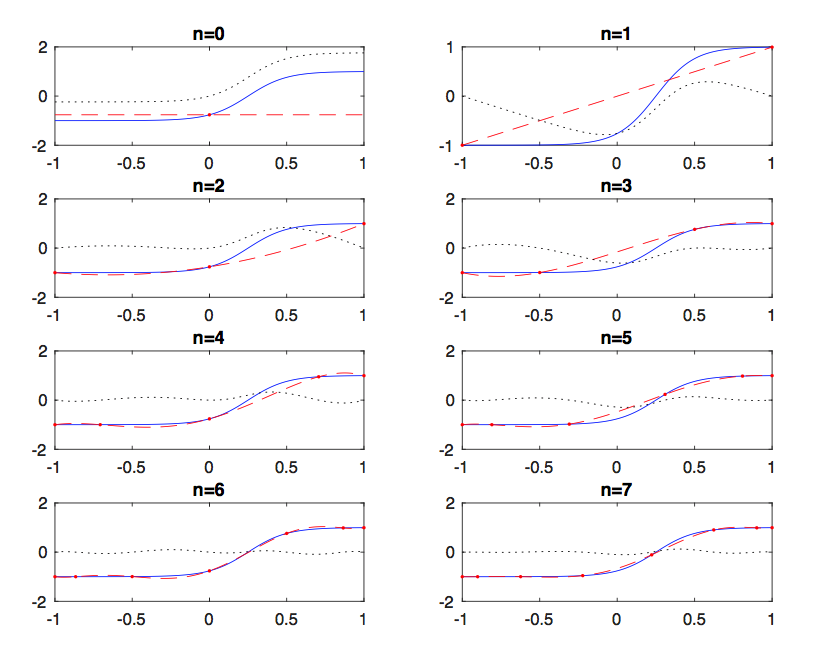
\includegraphics[width=15cm]{./Figures/20170926-interpolation-simulation}
  \label{fig:poly-interpolation-simulation}
%
%  \small{}
\end{figure}

\begin{verbatim}
x = chebfun('x');
f = tanh (4 * x -1);
n0=0;n1=1;n2=2;n3=3;n4=4;n5=5;n6=6;n7=7;
pn0 = chebfun(f,n0+1);
pn1 = chebfun(f, n1+1);
pn2 = chebfun(f, n2+1);
pn3 = chebfun(f, n3+1);
pn4 = chebfun(f, n4+1);
pn5 = chebfun(f, n5+1);
pn6 = chebfun(f, n6+1);
pn7 = chebfun(f, n7+1);

figure(1);
subplot(4,2,1),plot(f, '-b'), hold on, plot(pn0, '.--r'), hold on, plot(f-pn0, ':k'), title('n=0'),
subplot(4,2,2),plot(f, '-b'), hold on, plot(pn1, '.--r'), hold on, plot(f-pn1, ':k'), title('n=1'),
subplot(4,2,3),plot(f, '-b'), hold on, plot(pn2, '.--r'), hold on, plot(f-pn2, ':k'), title('n=2'),
subplot(4,2,4),plot(f, '-b'), hold on, plot(pn3, '.--r'), hold on, plot(f-pn3, ':k'), title('n=3'),
subplot(4,2,5),plot(f, '-b'), hold on, plot(pn4, '.--r'), hold on, plot(f-pn4, ':k'), title('n=4'),
subplot(4,2,6),plot(f, '-b'), hold on, plot(pn5, '.--r'), hold on, plot(f-pn5, ':k'), title('n=5'),
subplot(4,2,7),plot(f, '-b'), hold on, plot(pn6, '.--r'), hold on, plot(f-pn6, ':k'), title('n=6'),
subplot(4,2,8),plot(f, '-b'), hold on, plot(pn7, '.--r'), hold on, plot(f-pn7, ':k'), title('n=7'),
\end{verbatim}

\begin{theorem}[切比雪夫截断定理]
  \label{theorem:poly-cheby-truncation-theorem}
  切比雪夫截断定理(Chebyshev truncation theorem)\index{truncation!Chebyshev \dotfill 切比雪夫截断}是指,我们用$j$次切比雪夫多项式来近似未知的原方程系统$f(x)$,近似的误差小于等于一系列未被纳入考虑的更高次切比雪夫多项式系数之和,换句话说,定义$d^j(\cdot | \theta) = \sum_{i=0}^{j} \theta_i \psi_i(x)$,则截断误差(truncation error)
  \begin{equation}
    \label{eq:poly-cheby-truncation-theorem}
    d(x) - d^j(x|\theta) \le \sum_{i=j+1}^{\infty} \left| \theta_i \right|, \quad \forall x \in [-1,1], \quad \forall j.
  \end{equation}
\end{theorem}
\begin{proof}
  略。
\end{proof}


\begin{theorem}
  第$n$次一类切比雪夫多项式$T_n(x)$有$n$个根
  \begin{equation}
    \label{eq:poly-cheby-1-roots}
    x_i = \cos \left( \frac{2 i - 1}{2 n } \pi \right), \quad i = 1,2,\ldots, n,
  \end{equation}
  并且进而可将$T_n(x)$写为
  \begin{equation}
    \label{eq:poly-cheby-1-leadcoeff-root}
    T_n(x) = k_n \Pi_{i=0}^{n} \left(x - x_i \right) = 2^{n-1}  \Pi_{i=0}^{n} \left(x - x_i \right) , \quad i=1,2,\ldots,n.
  \end{equation}
\end{theorem}
\begin{proof}
  cf. \cite[p.49]{Boyd:2001wt}。
\end{proof}


\section{AR(1)过程的离散方法}
\label{sec:pj-local-discretization}
当未来存在不确定性时,求解经济个体行为最大化的问题便涉及条件期望的计算。以消费——储蓄决策问题为例,可表示为如下贝尔曼方程(Bellman equation)
\begin{equation}
  \label{sec:pj-local-discrete-cs-problem}
  \begin{split}
    &V(a, \lambda) = \max_{\{c, a' \}} \left\{ u(c) + \beta E\left[ V(a', \lambda') | \lambda \right]\right\}, \quad \text{s.t.}\\
    & a (1+r) + \omega \exp(\lambda) = a' + c, \\
    & \lambda' = (1-\rho) \mu_{\lambda} + \rho \lambda + \varepsilon,\quad \varepsilon \sim N(0,\sigma_{\varepsilon}^2), \\
    & c \ge 0, a' > 0.
  \end{split}
\end{equation}
其中状态矩$\lambda$的无条件均值和方差为$\lambda \sim N(\mu_{\lambda}, \sigma_{\lambda}^2)$。在给定$\lambda$的情况下,$\lambda'$是一个AR(1)过程,满足条件均值和方差$\lambda' \sim N\left( (1-\rho) \mu_{\lambda} + \rho \lambda, \sigma_{\varepsilon}^2 \right)$。$\sigma_{\varepsilon}$和$\sigma_{\lambda}$的关系满足
\begin{equation*}
  \sigma_{\lambda} = \frac{\sigma_{\varepsilon}}{\sqrt{1-\rho^2}}.
\end{equation*}

在此例中,涉及条件期望的计算目标是由$f(\lambda' | \lambda)$加权后的价值方程的积分值
\begin{equation}
  \label{eq:pj-local-discrete-cond-density-def}
  E\left[ V(a', \lambda') | \lambda \right] = \int_{-\infty}^{\infty} V(a',\lambda') f(\lambda' | \lambda) d \lambda',
\end{equation}
其中$f(\lambda' | \lambda)$指给定$\lambda$的情况下,$\lambda'$的条件密度(conditional density)\index{conditional density \dotfill 条件密度}。

上式是一个与当前期状态有关的无限维度问题,需要借助数值近似算法。一个可行的近似方案,思路为:将状态空间中原本是连续的状态,离散化变为有限个点,对这些点对应的条件期望做近似。换句话说,就是将关于连续的$\lambda$的马尔科夫链,转变为离散的有限马尔科夫链,我们将新的马尔科夫链用$\tilde{\lambda}$来予以区分。有限个数的$\tilde{\lambda}$取值可以来自$\Lambda = \{ \lambda_1, \lambda_2, \ldots \lambda_n \}$集合,对应转移矩阵$P$,含有转移概率$p_{i,j}$,满足
\begin{equation*}
  p_{i,j} = Prob \left( \tilde{\lambda}' = \lambda_j | \tilde{\lambda} = \lambda_i \right), \quad i,j=1,2,\ldots,n.
\end{equation*}

通过这种方式,原本是含有条件期望的积分计算问题\eqref{eq:pj-local-discrete-cond-density-def},被转换为离散化的求和问题,可以借助计算机,用某些特定的数值算法求得。下面分别介绍三种常见算法。

\subsection{Tauchen(1986)法}
\label{sec:pj-local-discretization-tauchen86}

\cite{Tauchen:1986gi}的方法可表示如下:

首先是$\lambda$的选取。在$\Lambda$中选取均匀分布的$n$个点$\{ \lambda_1, \lambda_2, \ldots \lambda_n \}$,其中$\lambda_{1}$和$\lambda_n$分别对应上下边界,值等于无条件均值$\mu_t$加上或减去无条件标准差$\sigma_{\lambda}$的$m$倍数
\begin{align*}
  &\lambda_1 = \mu_{\lambda} - m \sigma_{\lambda},\\
  &\lambda_2 = \mu_{\lambda} + m \sigma_{\lambda},
\end{align*}
经验研究中,$m$的取值通常在2到3之间。

随后是转移矩阵$P$的选取。设
\begin{equation*}
  \omega = \lambda_j - \lambda_{j-1},
\end{equation*}
进而
\begin{equation*}
  p_{i,j} = \begin{cases}
  Prob \left[ (1-\rho) \mu_{\lambda} + \rho \lambda_{i} + \varepsilon \le \lambda_{\{j=1\}}  + \frac{\omega}{2} \right] & \text{如果} j=1,\\
  Prob \left[
  \lambda_j - \frac{\omega}{2} \le (1-\rho) \mu_{\lambda} + \rho \lambda_{i} + \varepsilon \le \lambda_j + \frac{\omega}{2}
  \right] & \text{如果} j=2,3,\ldots,n-1,\\
  1-Prob \left[ \lambda_{\{j=n\}} + \frac{\omega}{2} \le (1-\rho) \mu_{\lambda} + \rho \lambda_{i} + \varepsilon  \right] & \text{如果} j=n.
  \end{cases}
\end{equation*}

上式进一步整理为
\begin{equation*}
  p_{i,j} = \begin{cases}
  \Phi \left( \frac{\lambda_1 + \frac{\omega}{2} - (1-\rho) \mu_{\lambda} - \rho \lambda_i}{\sigma_{\varepsilon}}\right) & \text{如果} j=1,\\
  \Phi \left(
  \frac{
  \lambda_j + \frac{\omega}{2} - (1-\rho) \mu_{\lambda} - \rho \lambda
  }{
  \sigma_{\varepsilon}
  } \right) -
  \Phi \left(
  \frac{
  \lambda_j - \frac{\omega}{2} - (1-\rho) \mu_{\lambda} - \rho \lambda
  }{
  \sigma_{\varepsilon}
  } \right)
   & \text{如果} j=2,3,\ldots,n-1,\\
  1- \Phi \left(
  \frac{
  \lambda_n - \frac{\omega}{2} - (1-\rho) mu_{\lambda} - \rho \lambda
  }{\sigma_{\varepsilon}}
  \right)& \text{如果} j=n,
  \end{cases}
\end{equation*}
其中$\Phi(\cdot)$表示标准正态累积分布函数(standard normal cumulative distribution function)。

\cite{Tauchen:1986gi}法,将$\tilde{\lambda}'|\tilde{\lambda} = \lambda_i$作为对$ \lambda'|\lambda = \lambda_i$的条件概率的离散近似。$n$越大,对节点的选取越密,近似的效果越精确。\cite{Tauchen:1986gi}指出当$n=9$时所获得的近似精度基本已能满足经验研究的一般需要\footnote{然而随着外生过程的持续性越来越强(high persistence)即$\rho \rightarrow 1$,近似的精度就越来越低,这就需要我们提高$n$的数量以弥补精度的下降,或是采取更适合离散化高持续性过程的算法,如第\ref{sec:pj-local-discretization-rouwenhorst95}节的\cite{Rouwenhorst:1995tq}法。}。

举例说明。对于一个随机AR(1)连续过程
\begin{equation*}
  z_t = 0.95 z_{t-1} + \varepsilon_t
\end{equation*}
以及正态分布$N(0,0.007^2)$而言,假定我们想要对它做离散化近似,对应$n=9$个点,$m=3$。

我们可以根据\cite{Tauchen:1986gi}的思路编写代码,或者使用现有程序。以Matlab为例,Iskander Karibzhanov在他的个人主页\footnote{\url{http://karibzhanov.com}。}提供了名为tauchen.m的程序。Matlab代码如下
\begin{verbatim}
  >> [y,P,d]=tauchen(5,0,0.95,0.007,3)

  y =

     -0.0673   -0.0336         0    0.0336    0.0673


  P =

      0.9727    0.0041    0.0000    0.0000    0.0000
      0.0273    0.9806    0.0082    0.0000    0.0000
      0.0000    0.0153    0.9837    0.0153    0.0000
           0    0.0000    0.0082    0.9806    0.0273
           0         0    0.0000    0.0041    0.9727


  d =

      0.0361    0.2392    0.4494    0.2392    0.0361
\end{verbatim}

即,我们得到了
\begin{equation*}
  z_t \in \left\{ -0.0673,   -0.0336,         0,    0.0336,    0.0673 \right\}
\end{equation*}

对应转移矩阵$P$
\begin{equation*}
P_{z,z'}=  \begin{pmatrix}
0.9727&    0.0041&    0&    0&    0\\
0.0273&    0.9806&    0.0082&    0&    0\\
0&    0.0153&    0.9837&    0.0153&    0\\
0&    0&    0.0082&    0.9806&    0.0273\\
0&         0&    0&    0.0041&    0.9727,
  \end{pmatrix}
\end{equation*}
需要注意的是$P_{z,z'}$对角元素接近于1,这说明随机过程的当期状态与上期状态高度相关(对应$\rho = 0.95$)。\cite{Tauchen:1986gi}增加$n$的值到9后,相关度仍然比较高(见下),这需要我们探讨其他数值算法,见第\ref{sec:pj-local-discretization-rouwenhorst95}节。

\begin{verbatim}
  >> [y,P,d]=tauchen(9,0,0.95,0.007,3)

  y =

     -0.0673   -0.0504   -0.0336   -0.0168         0    0.0168    0.0336    0.0504    0.0673


  P =

      0.7644    0.0592    0.0001    0    0    0    0    0    0
      0.2347    0.7405    0.0747    0.0001    0    0    0    0    0
      0.0009    0.1997    0.7569    0.0931    0.0002    0    0    0    0
      0    0.0006    0.1679    0.7669    0.1147    0.0002    0    0    0
      0    0    0.0004    0.1396    0.7702    0.1396    0.0004    0    0
           0    0    0    0.0002    0.1147    0.7669    0.1679    0.0006    0
           0         0    0    0    0.0002    0.0931    0.7569    0.1997    0.0009
           0         0         0    0    0    0.0001    0.0747    0.7405    0.2347
           0         0         0         0         0    0    0.0001    0.0592    0.7644


  d =

      0.0108    0.0428    0.1144    0.2064    0.2513    0.2064    0.1144    0.0428    0.0108

\end{verbatim}

即,我们得到了
\begin{equation*}
  z_t \in \left\{ -0.0673 ,  -0.0504,   -0.0336,   -0.0168,         0,    0.0168,    0.0336,    0.0504,    0.0673 \right\},
\end{equation*}
对应转移矩阵$P$
\begin{equation*}
P_{z,z'} = \begin{pmatrix}
0.7644&    0.0592&    0.0001&   0&    0&    0&    0&    0&    0 \\
0.2347&    0.7405&    0.0747&    0.0001&    0&    0&    0&    0&    0 \\
0.0009&    0.1997&    0.7569&    0.0931&    0.0002&    0&    0&    0&    0\\
0&    0.0006&    0.1679&    0.7669&    0.1147&    0.0002&    0&    0&    0\\
0&    0&    0.0004&    0.1396&    0.7702&    0.1396&    0.0004&    0&    0\\
0&    0&    0&    0.0002&    0.1147&    0.7669&    0.1679&    0.0006&    0\\
0&         0&    0&    0&    0.0002&    0.0931&    0.7569&    0.1997&    0.0009\\
0&         0&         0&    0&    0&    0.0001&    0.0747&    0.7405&    0.2347\\
0&         0&         0&         0&         0&    0&    0.0001&    0.0592&    0.7644\\
\end{pmatrix}
\end{equation*}



\subsection{Tauchen and Hussey (1991)法}
\label{sec:pj-local-discretization-th91}

同样对矩$\lambda$
而言,\cite{Tauchen:1991iv}使用高斯——埃米特求积(Gauss-Hermite quadrature)\index{Gauss-Hermite quadrature \dotfill 高斯——埃米特求积}去近似价值方程的条件期望积分,\eqref{eq:pj-local-discrete-cond-density-def}改写为
\begin{equation}
  \label{eq:pj-local-discrete-cond-density-gauss}
  E \left[ V(a', \lambda') | \lambda \right] \approx \frac{1}{\sqrt{\pi}} \sum_{j=1}^{n} \omega_j V(a', \sqrt{2} \sigma_\lambda \hat{\lambda}'_j + \mu_\lambda), \quad j=1,2,\ldots, n
\end{equation}
其中$ \hat{\lambda}'_j$是第$n$次埃米特多项式$H_n(\lambda)$的根(第\ref{sec:poly-hermite}节),满足
\begin{equation*}
  \lambda_j = \sqrt{2} \sigma_{\varepsilon} \hat{\lambda}_j + \mu_{\lambda},
\end{equation*}
$\omega_j$是对应$\hat{\lambda}'_j$的权重。

研究目标与\eqref{eq:pj-local-discrete-cond-density-def}相同:给定$\lambda$的情况下有AR(1)过程$\lambda'$,计算加权价值方程积分
\begin{equation*}
  E\left[ V(a', \lambda') | \lambda \right] = \int_{-\infty}^{\infty} V(a',\lambda') f(\lambda' | \lambda) d \lambda'.
\end{equation*}

原本可以采用上节\ref{sec:pj-local-discretization-tauchen86}介绍的\cite{Tauchen:1986gi}算法做近似求解,但需注意$\lambda'$的条件均值是一个关于$\lambda$的方程,这意味着对于每个不同的$\lambda$,都会有一组不同的$\lambda'$,进而迭代算出的集合$\Lambda$可能有无数个。为了避免这个问题,\cite{Tauchen:1991iv}建议使用如下转换
\begin{equation*}
\begin{split}
    E\left[ V(a', \lambda') | \lambda \right] &= \int_{-\infty}^{\infty} V(a',\lambda') f(\lambda' | \lambda) d \lambda'\\
    &= \int_{-\infty}^{\infty} V(a',\lambda') \frac{
    f(\lambda' | \lambda)
    }{f(\lambda' | \mu_{\lambda})}
    f(\lambda' | \mu_{\lambda}) d \lambda'.
\end{split}
\end{equation*}
其中$f(\lambda' | \mu_{\lambda})$表示在$\lambda$恰好等于其无条件均值$\mu_{\lambda}$的情况下,$\lambda'$的条件密度。将高斯——埃米特求积\eqref{eq:pj-local-discrete-cond-density-gauss}代入上式,可得
\begin{equation}
  \label{eq:pj-local-discrete-th1991-mid}
  \begin{split}
    &E\left[ V(a', \lambda') | \lambda \right] \approx
    \frac{1}{\sqrt{\pi}} \sum_{j=1}^{n} \omega_j V(a', \lambda_j) \frac{f(\lambda_j | \lambda)}{f(\lambda_j | \mu_{\lambda})}, \quad \text{其中} \\
    & \quad \lambda_j = \sqrt{2} \sigma_{\varepsilon} \hat{\lambda}_j + \mu_{\lambda}, \\
    & \quad \hat{\lambda}_j, j=1,2,\ldots,n \, \text{表示第n次埃米特多项式的根}, \\
    & \quad \omega_j \text{表示第n次埃米特多项式的根对应的权重}.
  \end{split}
\end{equation}

那么,对于$\lambda = \lambda_i$,我们有
\begin{equation}
  \label{eq:pj-local-discrete-th1991-midd}
  E \left[ V(a', \lambda' | \lambda) \right] \approx \sum_{j=1}^{n} \tilde{\omega}_{i,j} V(a', \lambda_i), \quad \tilde{\omega}_{i,j}= \frac{1}{\sqrt{\pi}} \omega_j \frac{
  f(\lambda_j | \lambda_i)
  }{
  f(\lambda_j | \mu_{\lambda})
  },
\end{equation}
上式意味着,我们选取$\tilde{\lambda}$的可能集合为
\begin{equation*}
  \Lambda = \left\{ \tilde{\lambda} | \lambda = \sqrt{2} \sigma_{\varepsilon} \hat{\lambda}_j, \, j=1,2,\ldots,n \right\},
\end{equation*}
选取$\tilde{w}$的可能集合为转移矩阵$P$:需要注意的是
\begin{equation*}
  \sum_{j=1}^{n} \tilde{\omega}_{i,j} \neq 1,
\end{equation*}
因此$P$中的元素
\begin{equation*}
  p_{i,j} = \frac{
  \tilde{\omega}_{i,j}
  }{
  \sum_{j=1}^{n} \omega_{i,j}
  }.
\end{equation*}

\eqref{eq:pj-local-discrete-th1991-midd}因此最终改写为
  \begin{equation}
    \label{eq:pj-local-discrete-th1991}
    E \left[ V \left( a', \tilde{\lambda}' | \lambda_i \right) \right] \approx \sum_{j=1}^{n} p_{i,j} V \left( a',\lambda_j \right).
  \end{equation}

由\eqref{eq:pj-local-discrete-th1991}可见,利用\cite{Tauchen:1991iv}近似条件期望用到高斯——埃米特求积的知识,但在实际计算过程中并不需要做高斯——埃米特求积\footnote{然而随着$n \rightarrow \infty$,我们有
\begin{equation*}
\lim_{n \rightarrow \infty} \sum_{j=1}^{n} \tilde{\omega}_{i,j} \rightarrow 1, \quad \forall i = 1,2,ldots,n,
\end{equation*}
因此\eqref{eq:pj-local-discrete-th1991}的\cite{Tauchen:1991iv}算出的条件期望近似依然是向高斯——埃米特求积法\eqref{eq:pj-local-discrete-cond-density-gauss}收敛的。}。

与\cite{Tauchen:1986gi}法相比,\cite{Tauchen:1991iv}的不同在于权重方程改用条件密度$\omega \left( \lambda' \right) = f \left( \lambda' | \mu_{\lambda} \right)$,如\eqref{eq:pj-local-discrete-th1991-mid}。与无条件密度相比,有条件密度在区间的中央赋予更多权重,在区间的两端赋予更小权重。这样一来,有条件密度作为权重方程,可以更好平衡两组互相冲突的原则:第一,一个好的近似总是会在无条件均值附近留下较多权重,第二,一个好的近似总是会使得在区间的两端,$\frac{f\left( \lambda' | \lambda \right)}{\omega(\lambda')}$比值不至于相对于$w(\lambda')$而增长过快。

Iskander Karibzhanov也提供了名为tauchenHussey.m的Matlab程序。

\subsection{Rouwenhorst(1995)法}
\label{sec:pj-local-discretization-rouwenhorst95}

如前文所述,对于高持续性$\rho \rightarrow 1$(如$\rho=0.9$)的过程来说,\cite{Tauchen:1986gi}近似法的精度较低。\cite{Kopecky:2010du}研究发现\cite{Rouwenhorst:1995tq}法在此时更为理想。

在区间$[\mu_{\lambda} - \nu, \mu_{\lambda} + \nu]$内选取对称且均匀分布的$n$个点构成$\Lambda$。用如下方法计算$P$:通过选择$p$和$p$,使得当时
\begin{equation*}
P_{n=2} = \begin{pmatrix}
p & 1-p \\
1-1 & q
\end{pmatrix}, \quad P_{n=3} = \begin{pmatrix}
p^2 & 2p (1-q) & (1-p)^2 \\
p(1-q) & pg + (1-p)(1-q) & q(1-p)\\
(1-q)^2 & 2q(1-p) & q^2
\end{pmatrix},
\end{equation*}
进而用递归方法,根据$P_{n-1}$计算$P_n$,分两步。首先将$n \times n$矩阵相加
\begin{equation*}
  p \begin{pmatrix}
    P_{n-1} & \bm{0} \\
    \bm{0}^{\top} & 0
    \end{pmatrix}
    + (1-p) \begin{pmatrix}
    \bm{0} & P_{n-1} \\
    0 & \bm{0}^{\top}
    \end{pmatrix},
\end{equation*}

\begin{equation*}
    (1-q) \begin{pmatrix}
    \bm{0}^{\top} & 0\\
    P_{n-1} & \bm{0}
    \end{pmatrix}
    + q \begin{pmatrix}
    0 & \bm{0}^{\top} \\
    \bm{0} & P_{n-1}
    \end{pmatrix},
\end{equation*}
随后将除了第一和最后一行之外的其他行都除以2。这样矩阵$P_n$的条件概率之和等于1。

$p^{n-1}$表示当期已处于最低状态时,下期仍处在最低状态的概率;$q^{n-1}$表示当期已处于最高状态时,下期仍处在最高状态的概率。$ (1-p)^{n-1} $表示当期已处于最低状态时,下期由最低转为最高状态的概率;$ (1-q)^{n-1} $表示当期已处于最高状态时,下期由最高转为最低状态的概率。对于任何$p \neq q$的情况,都会导致生成的冲击序列中出现异方差(heteroscedasticity)。

不论$n$和$\Lambda$的取值是怎样的,$\tilde{\lambda}$过程的一届序列相关性总是$p+q-1$。因此,如果我们设定$p+q = \pi$,就可以使得所生成的离散过程,具有和连续过程相同的一阶持续性$\rho$。

此外,$\tilde{\lambda}$的方差也总是$\frac{\nu^2}{n-1}$。因此对于某个给定的$n$值,1个合适的$\nu$值取值是使得\begin{equation*}
var \left( \tilde{\lambda} \right) = var \left( \lambda \right) \quad \Rightarrow \nu = \left( \frac{n-1}{\rho^2 - 1} \right)^{\frac{1}{2}} \sigma_{\varepsilon}.
\end{equation*}

Iskander Karibzhanov的matlab代码:

\begin{verbatim}
  >> rouwenhorst(0.95,0.007,5)

  ans =

     -0.0448   -0.0224         0    0.0224    0.0448

  >> rouwenhorst(0.95,0.007,7)

  ans =

     -0.0549   -0.0366   -0.0183         0    0.0183    0.0366    0.0549

  >> rouwenhorst(0.95,0.007,9)

  ans =

     -0.0634   -0.0476   -0.0317   -0.0159         0    0.0159    0.0317    0.0476    0.0634
\end{verbatim}

%\end{subappendices}

%!TEX root = ../DSGEnotes.tex
%\begin{subappendices}
\section{伽辽金近似}
\label{sec:pj-galerkin-approximation}

\subsection{举例:1维空间中的伽辽金近似}
\label{sec:pj-galerkin-1d-example}
以一个1维空间的有界极值问题为例,介绍伽辽金近似法(Galerkin approximation method)\index{Galerkin method \dotfill 伽辽金近似法}。假定$u(x)$是下述方程系统的解
\begin{equation}
  \label{eq:pj-galerkin-value-problem-1d}
  \begin{cases}
    -u'' + u = f, \quad \text{in} (0,1) \\
    u(0)=u(1)=0,
  \end{cases}
\end{equation}
我们的目标是找到一个对$u$的近似解。对上式两侧乘以一个检验方程$\nu$,然后分段积分,可得\eqref{eq:pj-galerkin-value-problem-1d}的弱条件形式\todo{弱条件补一个reference}
\begin{equation}
  \label{eq:pj-galerkin-value-problem-integral}
  \int_{0}^{1} \left( u' \nu' + u \nu \right) \, dx = \int_{0}^{1} f \, \nu dx, \quad \forall \nu \in H_{0}^1(0,1),
\end{equation}
 其中$ H_{0}^{1}(0,1) $是索伯列夫空间(Sobolev space)\index{Sobolev space! \dotfill 索伯列夫空间}。

如果方程$u$是常规方程,即连续且二阶可导\todo{补一个reference},那么\eqref{eq:pj-galerkin-value-problem-1d}与\eqref{eq:pj-galerkin-value-problem-integral}等价。这意味着我们可以利用\eqref{eq:pj-galerkin-value-problem-integral},构建一个多项式近似$u$。
将域$\left[ 0,1 \right]$划分为$N+1$个均匀分布(uniform distribution)的子域,每个域对应子空间$(x_j,x_{j+1})$,满足
 \begin{equation*}
   x_j = \frac{j}{N+1} \quad j=0,1, %\ldots,N+1.
 \end{equation*}

此外,定义一个包含检验方程$\nu$的空间$V_N$,满足
\begin{equation*}
  V_N = \left\{ \nu \in C^{0} : \nu |_{x_j,x_{j+1}} \text{是线性方程,并且  } \nu(0) = \nu(1) = 0 \right\},
\end{equation*}
其中$C^{0}$表示连续方程的空间。

$V_N$满足如下特征:首先,$V_N$是个有限维度空间,$N < \infty$。其次,$V_N \subset H_0^1(0,1) \, \forall N$。事实上,$\nu(x) \in V_N$由且仅由他所对应的有限个数的点$(x_1,x_2,\ldots,x_N)$所决定。

定义一个伽辽金近似方程$u_N \in V_N$作为对$u$的近似,代入\eqref{eq:pj-galerkin-value-problem-integral},我们有
\begin{equation}
  \label{eq:pj-galerkin-value-problem-approximate}
  \int_{0}^{1} \left( u_N' \nu' + u_N \nu \right) \, dx = \int_{0}^{1} f \, \nu \, dx, \quad \forall \nu \in V_N,
\end{equation}

由下节可知,存在且只存在一个$u_N$方程满足\eqref{eq:pj-galerkin-value-problem-approximate}条件\todo{解的存在性和唯一性}。并且由于$V_N$是个有限维度空间,因此$u_N$可以通过一些线性方程系统求解方法算得。基方程$\psi_j \in V_N$可以采取不同形式,例如可以选拉格朗日多项式(Lagrange polynomial)\index{polynomial!Lagrange \dotfill 拉格朗日多项式}
\begin{equation}
  \label{eq:pj-galerkin-psi-kronecker}
  \psi_j(x_i) = \delta_{ij}, \quad i,j=1,2,\ldots,N,
\end{equation}
其中$\delta_{ij}$表示克罗内克乘积。因此我们有近似方程
\begin{equation}
  \label{eq:pj-galerkin-approx-fun}
  u_N = \sum_{j=1}^{N} U_j \psi_j, \quad U_j \in \mathbb{R},
\end{equation}
其中$U_j := u_N(x_j)$。

既然任何一个检测方程$\nu \in V_N$都与$\psi_j$呈线性组合关系,\eqref{eq:pj-galerkin-value-problem-approximate}等价于
\begin{equation}
  \label{eq:pj-galerkin-value-problem-nupsik}
  \int_{0}^{1} \left( u_N' \psi_k' + u_N \psi_k \right) \, dx = \int_{0}^{1} f \, \psi_k \, dx, \quad k=1,2,\ldots,N.
\end{equation}

再引入\eqref{eq:pj-galerkin-approx-fun},替换上式LHS中的$u_N$,我们有
\begin{equation}
  \label{eq:pj-galerkin-value-problem-nupsik-uj}
  \sum_{j=1}^{N} U_j \int_{0}^1 \left( \psi_j' \psi_k' + \psi_j \psi_k \right) \, dx = \int_{0}^{1} f \, \psi_k \, dx, \quad k=1,2,\ldots,N.
\end{equation}

\eqref{eq:pj-galerkin-value-problem-nupsik-uj}构成一个$N$个方程的线性系统
\begin{equation}
  \label{eq:pj-galerkin-linear-sys}
\begin{split}
  A U = F&,\\
  &\begin{cases}
    \text{系数矩阵 } \, A=\left( a_{kj} \right) \in \mathbb{R}^{N \times N},& a_{kj} = \int_{0}^1 \left( \psi_j'\psi_k' + \psi_j \psi_k \right) \, dx,\\
    \text{系数矩阵 } \, F=\left( F_k \right) \in \mathbb{R}^{N}, & F_k = \int_{0,1}f \, \psi_k d_x,\\
    \text{待求解矩阵 } \, U=(U_j) \in \mathbb{R}^{N}
  \end{cases}
\end{split}
\end{equation}
通过求解线性方程系统\eqref{eq:pj-galerkin-linear-sys},可得矩阵$U$的解,进而根据\eqref{eq:pj-galerkin-approx-fun}可得$u_N$的值。


通过观察$\psi_j(x_i)$的性质\eqref{eq:pj-galerkin-psi-kronecker}可见,矩阵$A$是个对称的三角对角矩阵,对角元素及其附近不等于$0$的元素分别为
\begin{equation*}
  \begin{cases}
    a_{jj} = \frac{2}{h} + \frac{2}{3} h, \\
    a_{jj-1} = a_{jj+1} = -\frac{1}{h} + \frac{h}{6},
  \end{cases}
\end{equation*}
由此,待求解方程系统为$N+1$个等式
\begin{equation*}
  \begin{cases}
    U_0 := 0, \\
    \frac{-U_{j-1} + 2U_j - U_{j+1}}{h} + \frac{h}{6} U_{j-1} + \frac{2}{3} h U_j + \frac{h}{6} U_{j+1} = F_j, \quad j=1,2,\ldots,N,\\
    U_{j+1} := 0.
  \end{cases}
\end{equation*}
矩阵$A$是对称正定的(即$C^{\top} A C >0 \, \forall C \neq 0 $;由$a_{ij}$积分项中的双线性形式推得),由此可得$A$是可逆矩阵。因此,$U$进而$u_N$的解是唯一的\todo{解的存在性和唯一性}。

上式中两侧同时除以$h$,我们得到\eqref{eq:pj-galerkin-value-problem-1d}的有限差分近似形式
\begin{equation*}
  \underbrace{\frac{-U_{j-1} + 2U_j - U_{j+1}}{h^2}}_{\approx u''(x_j)} + \underbrace{\frac{1}{6} U_{j-1} + \frac{2}{3} U_j + \frac{1}{6} U_{j+1}}_{\approx u(x_j)} = \underbrace{\frac{1}{h}F_j}_{\approx f(x_j)}, \quad j=1,2,\ldots,N,
\end{equation*}
也就是说,在这个1维空间的例子中,伽辽金近似法就是将原求解问题转换为一个已知数量$N$的有限差分近似问题。

收敛问题。对于给定数量$N$,我们定义一个伽辽金近似$u_N \in V_N$,作为对原方程系统$u$的近似。随着$N \rightarrow \infty$,正交多项式的级数逐渐增加,可用来近似任何连续方程。换句话说,当空间集合$V_N$以如下方式近似$u$时,伽辽金近似$u_N$逐渐收敛至$u$:
\begin{equation*}
  \lim_{N \rightarrow \infty} ||u-v|| = \lim_{N \rightarrow \infty} \inf_{\nu \in V_{N} } ||u-v|| \rightarrow 0.
\end{equation*}

\subsection{伽辽金近似}
\label{sec:pj-galerkin-general}
第\ref{sec:pj-galerkin-1d-example}节以1维空间为例介绍了伽辽金近似的基本思路和方法。这节我们从1维扩展到通用情况,即在一个希尔伯特空间(Hilbert space)\index{Hilbert space \dotfill 希尔伯特空间}中,双线性形式下的伽辽金近似法\todo{补一个描述:Hilbert space}。

将一个希尔伯特空间定义为$V$,在其中定义一个双线性形式的连续方程$a(.,.)$和一个线性方程$L$,我们的研究目标是找到一个近似解$u \in V$,求解原方程系统
\begin{equation}
  \label{eq:pj-galerkin-prob}
  a \left( u,\nu \right) = \langle L, \nu \rangle, \quad \forall \, \nu \in V,
\end{equation}
其中$\langle .,. \rangle$表示在$V'$和$V$中的双内积(duality inner product)\index{inner product!duality \dotfill 双内积}\footnote{如$\langle A,B \rangle := A'B' + A B, \, \forall (A,B) \in V, \, (A',B') \in V'$。注意和\eqref{eq:poly-inner-product-def}的定义有所区别。}下面我们来分析,为了确保$u$存在唯一解,方程$a(.,.)$所应呈现的形式,即关于强制形式(coercive forms)\index{coercive form \dotfill 强制形式}的讨论。

\begin{definition}[方程的强制形式]
  如果存在一个常数$\alpha >0$,使得满足
  \begin{equation}
    \label{pj-galerkin-coercive-form-def}
    a(u,u) \ge \alpha ||u||_{V}^2, \quad \forall u \in V,
  \end{equation}
  那么我们说方程$a(.,.)$是一个$V$空间中的强制形式。
\end{definition}

举例说明,以\eqref{eq:pj-galerkin-prob}为例,对于二阶线形椭圆方程
  \begin{equation*}
    \begin{cases}
      -\sum_{i,j=1}^{n} \frac{\partial}{\partial x_i} \left( a_{ij} \frac{\partial u}{\partial x_j} \right) = f, & \text{in} \, \Omega \subset \mathbb{R}^n,\\
      u = 0, & \text{on} \partial \Omega
    \end{cases}
  \end{equation*}
  其中系数$a_{ij} = a_{ij}(x)$是有界方程。那么存在任意$\gamma > 0$使得
  \begin{equation}
    \label{eq:pj-galerkin-variational-form}
    \gamma |\xi|^2 \le \sum_{i,j=1}^n a_{ij} \xi_i \xi_j, \quad \forall x \in \Omega, \forall \xi \in \mathbb{R}^n,
  \end{equation}
或者说,可以以\eqref{eq:pj-galerkin-prob}的形式来表述,其中
\begin{itemize}
  \item 希尔伯特空间$V$
  \begin{equation*}
    V = H_{0}^{1}(\Omega) = \left\{ \nu \in L^2(\Omega) : \frac{\partial \nu}{\partial x_j} \in L^2(\Omega), \quad j=1,2,\ldots,n, \text{以及在}\, \partial \Omega \, \text{上有} \, \nu=0 \right\},
  \end{equation*}
  \item $\nu \in V$的范数(norm) \index{norm \dotfill 范数}为
  \begin{equation*}
    || \nu ||_{H^1} = ||\nu ||_{L^2} + ||\nabla \nu ||_{L^2},
  \end{equation*}
  \item $a(u,\nu)$为
  \begin{equation*}
    a(u,\nu) = \sum_{i,j=1}^n \int_{\Omega}a_{i,j} \frac{\partial u}{\partial x_i} \frac{\partial u}{\partial x_j} \, d x,
  \end{equation*}
  \item $L$满足
  \begin{equation*}
    \langle L, \nu \rangle = \int_{\Omega} f \, \nu \, dx.
  \end{equation*}
\end{itemize}

结合椭圆方程条件\eqref{eq:pj-galerkin-variational-form}、系数$a_{ij}$的有界特性以及庞加莱不等式,可得$a$函数形式是强制且连续的。线性方程形式$L$如果满足$f \in L^2$,则我们说它是连续的。

再举一个线性弹性方程的例子。对于应变——应力关系方程
\begin{equation*}
  \begin{cases}
    - \mu \Delta \bm{u} - (\lambda + \mu) \nabla div \bm{u} = \bm{f}, & \text{in} \, \Omega \subset \mathbb{R}^3, \\
    \bm{u} = 0, & \text{on} \, \partial \Omega
  \end{cases}
\end{equation*}
其中出于简化考虑,设满足齐次狄利克雷条件(homogeneous Dirichlet condition) \index{Dirichlet condition! homogeneous 齐次狄利克雷条件}。大于$0$的系数$\lambda$和$\mu$分别为拉梅第一参数和拉梅第二参数(Lamé elasticity parameters)\index{Lamé elasticity parameters \dotfill 拉梅弹性参数}。向量方程$\bm{u}$和$\bm{f}$未知。这个问题的弱形式可以表述为带有$V = H_{0}^{1} (\Omega)^3$条件的式\eqref{eq:pj-galerkin-prob},其中$a(\bm{u},\bm{v})$满足条件
\begin{equation*}
  a(\bm{u},\bm{v}) = \int_{\Omega} \left\{ 2 \mu \varepsilon_{i,j}(\bm{u}) \varepsilon_{i,j}(\bm{v}) + \lambda \, div \bm{u} \, div \bm{v} \, \right\} \, dx, \quad \varepsilon_{i,j} := \frac{1}{2} \left( \frac{\partial \nu_i}{\partial x_j} \frac{\partial \nu_j}{\partial x_i}\right).
\end{equation*}

进而,利用科恩不等式(Korn's inequality)\index{Korn inequality \dotfill 科恩不等式},我们有双线性形式的方程$a(.,.)$ \eqref{eq:pj-galerkin-prob} 是强制形式。

方程形式$a(.,.)$ \eqref{eq:pj-galerkin-prob}的解得存在性和唯一性,可由拉克斯一密格拉蒙定理(Lax-Milgram theorem, Theorem \ref{theorem:lax-milgram-lemma})\index{Lax-Milgram theorem \dotfill 拉克斯一密格拉蒙定理}予以证明。

在此基础上,上述条件也证实了伽辽金近似方程向原方程收敛。事实上,的确存在着一些重要范例如斯托克斯公式(Stokes equations)\index{Stokes equations \dotfill 斯托克斯公式}等,其中的双线性形式方程并不是强制的,但满足一个更弱的条件,称为上极限——下极限条件(inf-sup condition) \index{inf-sup condition \dotfill 上极限——下极限条件}\footnote{关于稳态斯托克斯公式弱形式的分析,以及上极限——下极限条件,可参考Chen Long的讲义 \href{https://www.math.uci.edu/~chenlong/226/infsup.pdf}{https://www.math.uci.edu/~chenlong/226/infsup.pdf}。}。
下面先介绍上线——下线极限条件定义。在第\ref{sec:pj-galerkin-convergence-coercive}节介绍双线性形式伽辽金近似的收敛问题。

\begin{definition}[上极限——下极限关系问题]

  如果双线性形式的方程$a(u,\nu)$在$V$空间上满足条件:对于某一$\alpha > 0$,有
  \begin{subequations}
    \label{eq:pj-galerkin-inf-sup-theorem}
    \begin{equation}
      \label{eq:pj-galerkin-inf-sup-theorem-u}
      \sup_{\nu \in V} \frac{a(u,\nu)}{||\nu||_{V}} \ge \alpha ||u||_{V}, \quad \forall u \in V,
    \end{equation}
    \begin{equation}
      \label{eq:pj-galerkin-inf-sup-theorem-nu}
      \sup_{u \in V} \frac{a(u,\nu)}{||u||_{V}} \ge \alpha ||\nu||_{V}, \quad \forall \nu \in V,
    \end{equation}
  \end{subequations}
  那么我们说,它满足上极限——下极限关系。
\end{definition}
根据这一定义,我们有以下推论:
\begin{enumerate}
\item 如果$a$是对称方程,\eqref{eq:pj-galerkin-inf-sup-theorem-u}和\eqref{eq:pj-galerkin-inf-sup-theorem-nu}等价。

\item 两个方程也可以写作
\begin{equation}
  \label{eq:pj-galerkin-inf-sup-theorem-analo}
  \inf_{u \in V} \sup_{\nu V} \frac{a(u,\nu)}{||u||_{V} \, ||\nu||_{V}}.
\end{equation}

\item 如果$a$是强制方程,那么它满足上极限——下极限关系,这是由于
\begin{equation}
  \label{eq:pj-galerkin-inf-sup-theorem-coersion}
  \sup_{\nu \in V} \frac{a(u,\nu)}{||\nu||_{V}} \ge \frac{a(u,\nu)}{||u||_{V}} \ge \alpha ||u||_{V}.
\end{equation}

\item 双线性方程$a$的上极限——下极限关系可以表示为关于$a$的线性算子$A$及其伴随算子$A^{*}$,
\begin{equation*}
  A:V \rightarrow V', \quad A^{*}: V \rightarrow V',
\end{equation*}
两个算子定义为
\begin{equation*}
  \begin{split}
    &\langle Au,\nu \rangle_{V' \times V} = a(u,\nu), \\
    &\langle u,A^{*} \nu \rangle_{V' \times V} = a(u,\nu),
  \end{split}
\end{equation*}
从而\eqref{eq:pj-galerkin-inf-sup-theorem-u}-\eqref{eq:pj-galerkin-inf-sup-theorem-nu}等价于
\begin{subequations}
  \label{eq:pj-galerkin-inf-sup-injection}
  \begin{equation}
    \label{eq:pj-galerkin-inf-sup-injection-A}
    ||A u||_{V'} \ge \alpha ||u||_{V}, \quad \forall u \in V,
  \end{equation}
  \begin{equation}
    \label{eq:pj-galerkin-inf-sup-injection-Astar}
    ||A^{*} \nu||_{V'} \ge \alpha ||\nu||_{V}, \quad \forall \nu \in V.
  \end{equation}
\end{subequations}

\item 当$V=\mathbb{R}^n$时,$a$的强制性意味着,其对应的矩阵$A$正定;$a$若满足上极限——下极限关系,则$A$进一步是可逆的。
\end{enumerate}

\begin{theorem}
  \label{theorem:galerkin-approximation}
  对于连续的双线性形式方程$a$,当且仅当线性算子$A$是双射(bijective)\index{bijection \dotfill 双射}的时,$a$满足上极限——下极限关系。$A$是双射的意思是说,原方程系统\eqref{eq:pj-galerkin-prob}对于任意$L \in V$都有唯一解,进而$A$有一个连续逆(continuous inverse)\index{continuous inverse \dotfill 连续逆}, 即$||u||_{V} \le C ||L||_{V'}$  \footnote{关于连续逆,可参考讲义Li Shiu-Tang的讲义
\href{http://www.math.utah.edu/\~li/Right\%20continuous\%20inverse.pdf}{http://www.math.utah.edu/\~li/Right\%20continuous\%20inverse.pdf}。}。
\end{theorem}
\begin{proof}
  根据泛函分析的基本原理可得,对于$W \subset V$,我们定义$W^{0} \subset V'$,满足
  \begin{equation*}
    W^0 \subset \left\{ L \in V': \langle L, \nu \rangle =0, \quad \forall \nu \in W \right\},
  \end{equation*}
  那么我们有
  \begin{subequations}
    \label{eq:pj-galerkin-bijection}
    \begin{equation}
      \label{eq:pj-galerkin-bijection-A}
      (Ker A)^0 = \overline{\Im{A^{*}}},
    \end{equation}
    \begin{equation}
      \label{eq:pj-galerkin-bijection-Astar}
      (Ker A^{*})^0 = \overline{\Im{A}},
    \end{equation}
    其中$\Im{(\cdot)}$表示复数的虚部(imaginary part)\index{complex number!imaginary part \dotfill 虚部(复数)};对应地,复数的实部(real part)\index{complex number!real part \dotfill 实部(复数)}表示为$\Re(\cdot)$。
  \end{subequations}

如果假定$a$满足上极限——下极限关系,那么由\eqref{eq:pj-galerkin-inf-sup-injection-A}可得$A$是单射(injective)\index{injection \dotfill 单射}的,由\eqref{eq:pj-galerkin-inf-sup-injection-Astar}可得$A^{*}$也是单射的。进而,如果我们能证明$\Im A$是封闭集,则根据\eqref{eq:pj-galerkin-bijection-Astar}可以证明定理。

假定$A u_n \mapsto w$,则由\eqref{eq:pj-galerkin-inf-sup-injection-A}可得
\begin{equation*}
  || A(u_n - u_m) ||_{V'} \ge \alpha || u_n - u_m ||_{V},
\end{equation*}
由此可见$\{u_n\}$是一个柯西序列(Cauchy sequnce)\index{Cauchy sequnce \dotfill 柯西序列},$u_n$收敛向某一个$u \in V$,并且由$A$的连续性特征可得,$w = A u \in \Im A$。

同理可得,如果$A$是双射的,那么$A^{*}$也是双射的,$A$和$A^{*}$都有一个连续逆。因此\eqref{eq:pj-galerkin-inf-sup-theorem-u}-\eqref{eq:pj-galerkin-inf-sup-theorem-nu}成立。
\end{proof}

在此基础上,我们为原方程系统\eqref{eq:pj-galerkin-prob}作伽辽金近似解。假定在$V$空间内,我们有一个有限维度的子空间$V_N$。则对原方程系统的伽辽金近似$u_N \in V_N$可定义为
\begin{equation}
\label{eq:pj-galerkin-approximation-solution}
a(u_N,\nu) = \langle L, \nu \rangle, \quad \forall \nu \in V_N.
\end{equation}

为了让$u_N$定义良好(well defined),我们需要对$a$作出限定。根据Theorem \ref{theorem:galerkin-approximation}可得当且仅当$a$在$V_N$子空间中满足上极限——下极限关系时,伽辽金近似解$u_N$才是存在且唯一的。尤其是,伽辽金近似解$u_N$对于强制形式的方程$a$是定义良好的。

从这个角度出发,有必要指出一下两种$V$中方程形式的本质区别:一种是强制形式,另一种是满足上极限——下极限关系,但并不是强制形式的:
\begin{remark}
  \label{remark:pj-galerkin-inf-sup-problem}
  如果$a$在$V$上强制,那么它在$V$的任何一个子空间中,尤其是$V_N$中都是强制的,此时伽辽金近似解$u_N$定义完备。

  但$V$上的上极限——下极限关系,无法传导到$V$的子空间中,那么对于不满足强制性的方程形式,还需要在子空间$V_N$中重新检验,以确保$u_N$定义完备。
\end{remark}


\subsection{强制型方程形式的伽辽金近似收敛}
\label{sec:pj-galerkin-convergence-coercive}
假定我们已知双线性形式方程$a(.,.)$是连续和强制的。因此我们有
\begin{equation}
  \label{eq:pj-galerkin-convergence-M}
  a(u,\nu) \le M  \, ||u||_{V} ||\nu||_{V}, \quad \forall u,\nu \in V,
\end{equation}
其中$M$定义为一个连续性常数(continuity constant)。在采用伽辽金近似法求得近似解$u_N$后,一个自然出现的问题是:在$V_N$被恰当选取的前提下,是否会出现$\lim_{N \rightarrow \infty} u_N \rightarrow u$的收敛?

显然,如果答案是肯定的,那么
\begin{equation}
  \label{eq:pj-galerkin-convergence-question}
  d(u,V_n) = \inf_{\nu \in V_n} || u - \nu ||_{V} \rightarrow 0, \quad \text{随着} \, N \rightarrow \infty.
\end{equation}
换句话说,收敛与否的问题,等价于探讨在子空间$V_{N}$中\eqref{eq:pj-galerkin-convergence-question}是否成立\footnote{子空间$V_N$中的所有方程,都是对$u$的近似。},以及它是不是收敛的充要条件。根据齐亚引理(Céa's lemma)\index{Céa lemma, \dotfill 齐亚引理},答案是肯定的。

\begin{lemma}[齐亚引理]
  \label{lemma:pj-galerkin-cea-lemma}
  如果$a$是一个连续且强制的方程,那么我们有
  \begin{equation}
    \label{eq:pj-galerkin-cea-lemma}
    ||u - u_N || _{V} \le \frac{M}{\alpha} \inf_{\nu \in V_N} || u - \nu || _{V}
  \end{equation}
\end{lemma}
\begin{proof}
  将伽辽金近似解 \eqref{eq:pj-galerkin-approximation-solution}
  和\eqref{eq:pj-galerkin-convergence-M}联立,构成误差方程
  \begin{equation}
    \label{eq:pj-galerkin-error-function}
    a(u-u_n,\nu)=0, \quad \forall \nu \in V_N.
  \end{equation}

由\eqref{eq:pj-galerkin-convergence-M}, ,\eqref{eq:pj-galerkin-convergence-question}和 \eqref{eq:pj-galerkin-error-function}我们有
  \begin{equation*}
    \alpha ||u-u_N||^2 \le a(u-u_N, u-u_N) = a(u - u_N,u-\nu) \le M ||u-u_N||_{V} ||u-\nu||_{V},
  \end{equation*}
  因此
  \begin{equation*}
    ||u-u_N|| \le M ||u-u_N||_{V} ||u-\nu||_{V}, \forall \nu \in V_N,
  \end{equation*}
  证毕。
\end{proof}

根据齐亚引理,在子空间$V_N$中,伽辽金近似解$u_N$是对原方程系统解$u$最好的近似,它除了受一个常数影响外,但只受双线性方程$a$形式的影响,而与子空间$V_N$的情况无关。根据这一特征,我们可以引出伽辽金近似解的收敛特性。

\begin{theorem}[伽辽金近似解的收敛(强制形式)]
  \label{theorem:pj-galerkin-approximation-convergence}
  如果$a$是个连续且强制的方程,并且空间$V_N$满足  \eqref{eq:pj-galerkin-convergence-question},那么我们有
  \begin{equation*}
    \lim_{N \rightarrow \infty} u_N = u.
  \end{equation*}
\end{theorem}

来讨论一个特殊情况,$a$还额外具有对称性。那么在$V$上,$a$定义了一个标量积(scalar product),这个标量积与原方程系统相同。此时,误差方程\eqref{eq:pj-galerkin-error-function}表明伽辽金近似解$u_N$恰好就是$u$在子空间$V_N$上的正交映射,对应标量积方程$a$。此时标量积$a$所对应的范就提供了最佳近似解。并且对应地,齐亚引理中的常数项$M/\alpha$变为$\sqrt{M/\alpha}$。

\subsection{仅满足上极限——下极限关系方程形式的伽辽金近似收敛}
\label{sec:pj-galerkin-convergence-infsup}
现在假定$a$不是强制的,但满足上极限——下极限关系\eqref{eq:pj-galerkin-inf-sup-theorem-u}-\eqref{eq:pj-galerkin-inf-sup-theorem-nu}。已知原方程系统\eqref{eq:pj-galerkin-prob}有唯一解,我们来讨论一下此时伽辽金近似的收敛问题。如Remark \ref{remark:pj-galerkin-inf-sup-problem}所强调的,上极限——下极限关系无法从$V$向下传递到子空间$V_N$,因此为了让伽辽金近似是定义良好的,我们需要假定$a$也在子空间$V_N$中满足上极限——下极限关系,即存在一个系数$\beta > 0$,使得
\begin{subequations}
  \begin{equation}
    \label{eq:pj-galerkin-approx-inf-sup-u}
    \sup_{\nu \in V_N} \frac{a(u,\nu)}{||\nu||_{V}} \ge \beta ||u||_{V}, \quad \forall u \in V_N.
  \end{equation}
  \begin{equation}
    \label{eq:pj-galerkin-approx-inf-sup-nu}
    \sup_{u \in V_N} \frac{a(u,\nu)}{||u||_{V}} \ge \beta ||\nu||_{V}, \quad \forall \nu \in V_N
  \end{equation}
\end{subequations}
我们证明\eqref{eq:pj-galerkin-approx-inf-sup-u}即可。这是因为既然子空间$V_N$是有限维度的,那么一旦\eqref{eq:pj-galerkin-approx-inf-sup-u}成立,\eqref{eq:pj-galerkin-approx-inf-sup-nu}也同样成立。

收敛若要存在,需要假定$\beta$不依赖于$N$。进而,\cite{Babuska:1971fx}对齐亚引理 \ref{lemma:pj-galerkin-cea-lemma}作以扩展,据此可以对Theorem \ref{theorem:pj-galerkin-approximation-convergence}作扩展。
\begin{lemma}[扩展齐亚引理]
  \label{lemma:pj-galerkin-cea-lemma-genralization}
  如果$a$是连续方程,满足\eqref{eq:pj-galerkin-approx-inf-sup-u}的上极限——下极限关系,那么
  \begin{equation*}
    ||u - u_N||_{V} \le \left( \frac{\beta + M}{\beta}\right) \inf_{\nu \in V_N} || u - \nu ||_{V},
  \end{equation*}
  尤其是当$\beta$不依赖于$N$时,误差项中的常数也不依赖于$N$。
\end{lemma}
\begin{proof}
  取$\nu \in V_N$。由\eqref{eq:pj-galerkin-approx-inf-sup-u}及误差方程\eqref{eq:pj-galerkin-error-function}可得
  \begin{equation*}
    \beta || \nu - u_N || _{V}
    \le \sup_{w \in V_N} \frac{a(\nu - u_N, w)}{||w||_{V}}
    = \sup_{w \in V_N} \frac{a(\nu-u, w)}{||w||_{V}}
    \le M ||\nu - u||_{V}.
  \end{equation*}
\end{proof}
由此我们有收敛定理:
\begin{theorem}[伽辽金近似解的收敛(上极限——下极限形式)]
  \label{theorem:pj-galerkin-approximation-limit-convergence}
  如果$a$是个连续方程,满足上极限——下极限关系\eqref{eq:pj-galerkin-approx-inf-sup-u},$\beta$不依赖于$N$,并且子空间$V_N$满足\eqref{eq:pj-galerkin-convergence-question},那么我们有
  \begin{equation*}
    \lim_{N \rightarrow \infty} u_N = u.
  \end{equation*}
\end{theorem}
